\documentclass[12pt]{article}

\usepackage{algorithmic}
\usepackage{algorithm}
\usepackage{alltt}
\usepackage{amsbsy}
\usepackage{amscd}
\usepackage{amsfonts}
\usepackage{amsmath}
\usepackage{amssymb}
\usepackage{amsthm}
\usepackage{booktabs}
\usepackage{eepic}
\usepackage{epic}
\usepackage{epsfig}
\usepackage{euscript}
\usepackage{fancyhdr}
\usepackage{float}
\usepackage{fullpage}
\usepackage{graphicx}
\usepackage{ifthen}
\usepackage{multirow}
\usepackage{supertabular}
\usepackage{times}
\usepackage{verbatim}
\usepackage{xspace}
\usepackage[colorlinks]{hyperref}
\usepackage[numbers,sort&compress]{natbib}
\usepackage[FIGBOTCAP,TABTOPCAP,bf,tight]{subfigure}

\usepackage[T1]{fontenc}
\usepackage{ae,aecompl}

\newtheorem{proposition}{Proposition}

%%%%%%%%%%%%%%%%%%%%%%%%%%%%%%%%%%%%%%%%%%%%%%%%%%%%%%%%%%%%%%%%%%%%%%%%
% editing
%%%%%%%%%%%%%%%%%%%%%%%%%%%%%%%%%%%%%%%%%%%%%%%%%%%%%%%%%%%%%%%%%%%%%%%%
%\usepackage[usenames,dvipsnames]{xcolor}
%\newcommand{\comment}[1]{\textcolor{blue}{[ \sc{#1} ]}} % comments
%\newcommand{\revise}[1]{\textcolor{red}{{#1}}} % revisions

%%%%%%%%%%%%%%%%%%%%%%%%%%%%%%%%%%%%%%%%%%%%%%%%%%%%%%%%%%%%%%%%%%%%%%%%
% abbreviations
%%%%%%%%%%%%%%%%%%%%%%%%%%%%%%%%%%%%%%%%%%%%%%%%%%%%%%%%%%%%%%%%%%%%%%%%
\newcommand{\aref}[1]{{App.~\ref{#1}}}
\newcommand{\eref}[1]{{Eq.~(\ref{#1})}}
\newcommand{\cref}[1]{{Ref.~\cite{#1}}}
\newcommand{\sref}[1]{{Sec.~\ref{#1}}}
\newcommand{\fref}[1]{{Fig.~\ref{#1}}}
\newcommand{\tref}[1]{{Table~\ref{#1}}}
\newcommand{\cf}{{cf.\,}}
\newcommand{\ie}{{i.e.\,}}
\newcommand{\vs}{{vs.\,}}
\newcommand{\eg}{{e.g.\,}}
\newcommand{\etal}{{et al.\,}}

%%%%%%%%%%%%%%%%%%%%%%%%%%%%%%%%%%%%%%%%%%%%%%%%%%%%%%%%%%%%%%%%%%%%%%%%
% tensors
%%%%%%%%%%%%%%%%%%%%%%%%%%%%%%%%%%%%%%%%%%%%%%%%%%%%%%%%%%%%%%%%%%%%%%%%
\renewcommand{\vec}[1]{{\boldsymbol{#1}}}
\newcommand{\chib}{\vec{\chi}}

%% suffix
\newcommand{\ab}{\vec{a}}
%\newcommand{\bb}{\vec{b}}
\newcommand{\vb}{\vec{v}}
\newcommand{\Ab}{\vec{A}}
\newcommand{\Bb}{\vec{B}}
\newcommand{\Tb}{\vec{T}}

%% prefix
\newcommand{\bzero}{\vec{0}}
\newcommand{\bone}{\vec{1}}

\newcommand{\bA}{\vec{A}}
\newcommand{\bB}{\vec{B}}
\newcommand{\bC}{\vec{C}}
\newcommand{\bD}{\vec{D}}
\newcommand{\bE}{\vec{E}}
\newcommand{\bF}{\vec{F}}
\newcommand{\bG}{\vec{G}}
\newcommand{\bH}{\vec{H}}
\newcommand{\bI}{\vec{I}}
\newcommand{\bJ}{\vec{J}}
\newcommand{\bK}{\vec{K}}
\newcommand{\bL}{\vec{L}}
\newcommand{\bM}{\vec{M}}
\newcommand{\bN}{\vec{N}}
\newcommand{\bO}{\vec{O}}
\newcommand{\bP}{\vec{P}}
\newcommand{\bQ}{\vec{Q}}
\newcommand{\bR}{\vec{R}}
\newcommand{\bS}{\vec{S}}
\newcommand{\bT}{\vec{T}}
\newcommand{\bU}{\vec{U}}
\newcommand{\bV}{\vec{V}}
\newcommand{\bW}{\vec{W}}
\newcommand{\bX}{\vec{X}}
\newcommand{\bY}{\vec{Y}}
\newcommand{\bZ}{\vec{Z}}

\newcommand{\ba}{\vec{a}}
\newcommand{\bb}{\vec{b}}
\newcommand{\bc}{\vec{c}}
\newcommand{\bd}{\vec{d}}
\newcommand{\be}{\vec{e}}
%\renewcommand{\bf}{\vec{f}}
\newcommand{\bff}{\vec{f}}
\newcommand{\bg}{\vec{g}}
\newcommand{\bh}{\vec{h}}
\newcommand{\bi}{\vec{i}}
\newcommand{\bj}{\vec{j}}
\newcommand{\bk}{\vec{k}}
\newcommand{\bl}{\vec{l}}
\newcommand{\bm}{\vec{m}}
\newcommand{\bn}{\vec{n}}
\newcommand{\bo}{\vec{o}}
\newcommand{\bp}{\vec{p}}
\newcommand{\bq}{\vec{q}}
\newcommand{\br}{\vec{r}}
\newcommand{\bs}{\vec{s}}
\newcommand{\bt}{\vec{t}}
\newcommand{\bu}{\vec{u}}
\newcommand{\bv}{\vec{v}}
\newcommand{\bw}{\vec{w}}
\newcommand{\bx}{\vec{x}}
\newcommand{\by}{\vec{y}}
\newcommand{\bz}{\vec{z}}

\newcommand{\balpha}{\vec{\alpha}}
\newcommand{\bbeta}{\vec{\beta}}
\newcommand{\bgamma}{\vec{\gamma}}
\newcommand{\bdelta}{\vec{\delta}}
\newcommand{\bepsilon}{\vec{\epsilon}}
\newcommand{\bvarepsilon}{\vec{\varepsilon}}
\newcommand{\bzeta}{\vec{\zeta}}
\newcommand{\beeta}{\vec{\eta}}
\newcommand{\btheta}{\vec{\theta}}
\newcommand{\bvartheta}{\vec{\vartheta}}
\newcommand{\bkappa}{\vec{\kappa}}
\newcommand{\blambda}{\vec{\lambda}}
\newcommand{\bmu}{\vec{\mu}}
\newcommand{\bnu}{\vec{\nu}}
\newcommand{\bxi}{\vec{\xi}}
\newcommand{\bomicron}{\vec{o}}
\newcommand{\bpi}{\vec{\pi}}
\newcommand{\bvarpi}{\vec{\varpi}}
\newcommand{\brho}{\vec{\rho}}
\newcommand{\bvarrho}{\vec{\varrho}}
\newcommand{\bsigma}{\vec{\sigma}}
\newcommand{\bvarsigma}{\vec{\varsigma}}
\newcommand{\btau}{\vec{\tau}}
\newcommand{\bupsilon}{\vec{\upsilon}}
\newcommand{\bphi}{\vec{\phi}}
\newcommand{\bvarphi}{\vec{\varphi}}
\newcommand{\bchi}{\vec{\chi}}
\newcommand{\bpsi}{\vec{\psi}}
\newcommand{\bomega}{\vec{\omega}}

\newcommand{\bGamma}{\vec{\Gamma}}
\newcommand{\bDelta}{\vec{\Delta}}
\newcommand{\bTheta}{\vec{\Theta}}
\newcommand{\bLambda}{\vec{\Lambda}}
\newcommand{\bXi}{\vec{\Xi}}
\newcommand{\bPi}{\vec{\Pi}}
\newcommand{\bSigma}{\vec{\Sigma}}
\newcommand{\bUpsilon}{\vec{\Upsilon}}
\newcommand{\bPhi}{\vec{\Phi}}
\newcommand{\bPsi}{\vec{\Psi}}
\newcommand{\bOmega}{\vec{\Omega}}

%%%%%%%%%%%%%%%%%%%%%%%%%%%%%%%%%%%%%%%%%%%%%%%%%%%%%%%%%%%%%%%%%%%%%%%%
% matrix
%%%%%%%%%%%%%%%%%%%%%%%%%%%%%%%%%%%%%%%%%%%%%%%%%%%%%%%%%%%%%%%%%%%%%%%%
\newcommand{\mat}[1]{\mathsf{#1}}
\newcommand{\transpose}[1]{{#1}^{\text{T}}}
\newcommand{\conjtransla}[1]{{#1}^{\text{*}}}
\newcommand{\conjtransqm}[1]{{#1}^{\dagger}}

%% suffix
\newcommand{\ws}{\mat{w}}
\newcommand{\As}{\mat{A}}
\newcommand{\Ms}{\mat{M}}

%% prefix
\newcommand{\szero}{\mat{0}}
\newcommand{\sone}{\mat{1}}

\newcommand{\sA}{\mat{A}}
\newcommand{\sB}{\mat{B}}
\newcommand{\sC}{\mat{C}}
\newcommand{\sD}{\mat{D}}
\newcommand{\sE}{\mat{E}}
\newcommand{\sF}{\mat{F}}
\newcommand{\sG}{\mat{G}}
\newcommand{\sH}{\mat{H}}
\newcommand{\sI}{\mat{I}}
\newcommand{\sJ}{\mat{J}}
\newcommand{\sK}{\mat{K}}
\newcommand{\sL}{\mat{L}}
\newcommand{\sM}{\mat{M}}
\newcommand{\sN}{\mat{N}}
\newcommand{\sO}{\mat{O}}
\newcommand{\sP}{\mat{P}}
\newcommand{\sQ}{\mat{Q}}
\newcommand{\sR}{\mat{R}}
\newcommand{\sS}{\mat{S}}
\newcommand{\sT}{\mat{T}}
\newcommand{\sU}{\mat{U}}
\newcommand{\sV}{\mat{V}}
\newcommand{\sW}{\mat{W}}
\newcommand{\sX}{\mat{X}}
\newcommand{\sY}{\mat{Y}}
\newcommand{\sZ}{\mat{Z}}

\newcommand{\sa}{\mat{a}}
\renewcommand{\sb}{\mat{b}}
\renewcommand{\sc}{\mat{c}}
\newcommand{\sd}{\mat{d}}
\newcommand{\se}{\mat{e}}
\renewcommand{\sf}{\mat{f}}
\newcommand{\sg}{\mat{g}}
\newcommand{\sh}{\mat{h}}
\newcommand{\si}{\mat{i}}
\newcommand{\sj}{\mat{j}}
\newcommand{\sk}{\mat{k}}
\renewcommand{\sl}{\mat{l}}
\newcommand{\sm}{\mat{m}}
\newcommand{\sn}{\mat{n}}
\newcommand{\so}{\mat{o}}
\renewcommand{\sp}{\mat{p}}
\newcommand{\sq}{\mat{q}}
\newcommand{\sr}{\mat{r}}
\renewcommand{\ss}{\mat{s}}
\newcommand{\st}{\mat{t}}
\newcommand{\su}{\mat{u}}
\newcommand{\sv}{\mat{v}}
\newcommand{\sw}{\mat{w}}
\newcommand{\sx}{\mat{x}}
\newcommand{\sy}{\mat{y}}
\newcommand{\sz}{\mat{z}}

\newcommand{\salpha}{\mat{\alpha}}
\newcommand{\sbeta}{\mat{\seta}}
\newcommand{\sgamma}{\mat{\gamma}}
\newcommand{\sdelta}{\mat{\delta}}
\newcommand{\sepsilon}{\mat{\epsilon}}
\newcommand{\svarepsilon}{\mat{\varepsilon}}
\newcommand{\szeta}{\mat{\zeta}}
\newcommand{\seta}{\mat{\eta}}
\newcommand{\stheta}{\mat{\theta}}
\newcommand{\svartheta}{\mat{\vartheta}}
\newcommand{\skappa}{\mat{\kappa}}
\newcommand{\slambda}{\mat{\lambda}}
\newcommand{\smu}{\mat{\mu}}
\newcommand{\snu}{\mat{\nu}}
\newcommand{\sxi}{\mat{\xi}}
\newcommand{\somicron}{\mat{o}}
\newcommand{\spi}{\mat{\pi}}
\newcommand{\svarpi}{\mat{\varpi}}
\newcommand{\srho}{\mat{\rho}}
\newcommand{\svarrho}{\mat{\varrho}}
\newcommand{\ssigma}{\mat{\sigma}}
\newcommand{\svarsigma}{\mat{\varsigma}}
\newcommand{\stau}{\mat{\tau}}
\newcommand{\supsilon}{\mat{\upsilon}}
\newcommand{\sphi}{\mat{\phi}}
\newcommand{\svarphi}{\mat{\varphi}}
\newcommand{\schi}{\mat{\chi}}
\newcommand{\spsi}{\mat{\psi}}
\newcommand{\somega}{\mat{\omega}}

\newcommand{\sGamma}{\mat{\Gamma}}
\newcommand{\sDelta}{\mat{\Delta}}
\newcommand{\sTheta}{\mat{\Theta}}
\newcommand{\sLambda}{\mat{\Lambda}}
\newcommand{\sXi}{\mat{\Xi}}
\newcommand{\sPi}{\mat{\Pi}}
\newcommand{\sSigma}{\mat{\Sigma}}
\newcommand{\sUpsilon}{\mat{\Upsilon}}
\newcommand{\sPhi}{\mat{\Phi}}
\newcommand{\sPsi}{\mat{\Psi}}
\newcommand{\sOmega}{\mat{\Omega}}

%%%%%%%%%%%%%%%%%%%%%%%%%%%%%%%%%%%%%%%%%%%%%%%%%%%%%%%%%%%%%%%%%%%%%%%%
% fourth-order tensors, common number sets
% latin/roman symbols only for now
%%%%%%%%%%%%%%%%%%%%%%%%%%%%%%%%%%%%%%%%%%%%%%%%%%%%%%%%%%%%%%%%%%%%%%%%

%% suffix

%% prefix
\newcommand{\bbA}{\mathbb{A}}
\newcommand{\bbB}{\mathbb{B}}
\newcommand{\bbC}{\mathbb{C}}
\newcommand{\bbD}{\mathbb{D}}
\newcommand{\bbE}{\mathbb{E}}
\newcommand{\bbF}{\mathbb{F}}
\newcommand{\bbG}{\mathbb{G}}
\newcommand{\bbH}{\mathbb{H}}
\newcommand{\bbI}{\mathbb{I}}
\newcommand{\bbJ}{\mathbb{J}}
\newcommand{\bbK}{\mathbb{K}}
\newcommand{\bbL}{\mathbb{L}}
\newcommand{\bbM}{\mathbb{M}}
\newcommand{\bbN}{\mathbb{N}}
\newcommand{\bbO}{\mathbb{O}}
\newcommand{\bbP}{\mathbb{P}}
\newcommand{\bbQ}{\mathbb{Q}}
\newcommand{\bbR}{\mathbb{R}}
\newcommand{\bbS}{\mathbb{S}}
\newcommand{\bbT}{\mathbb{T}}
\newcommand{\bbU}{\mathbb{U}}
\newcommand{\bbV}{\mathbb{V}}
\newcommand{\bbW}{\mathbb{W}}
\newcommand{\bbX}{\mathbb{X}}
\newcommand{\bbY}{\mathbb{Y}}
\newcommand{\bbZ}{\mathbb{Z}}

\newcommand{\bba}{\mathbb{a}}
\newcommand{\bbb}{\mathbb{b}}
\newcommand{\bbc}{\mathbb{c}}
\newcommand{\bbd}{\mathbb{d}}
\newcommand{\bbe}{\mathbb{e}}
\newcommand{\fb}{\mathbb{f}}
\newcommand{\bbg}{\mathbb{g}}
\newcommand{\bbh}{\mathbb{h}}
\newcommand{\bbi}{\mathbb{i}}
\newcommand{\bbj}{\mathbb{j}}
\newcommand{\bbk}{\mathbb{k}}
\newcommand{\bbl}{\mathbb{l}}
\newcommand{\bbm}{\mathbb{m}}
\newcommand{\bbn}{\mathbb{n}}
\newcommand{\bbo}{\mathbb{o}}
\newcommand{\bbp}{\mathbb{p}}
\newcommand{\bbq}{\mathbb{q}}
\newcommand{\bbr}{\mathbb{r}}
\newcommand{\bbs}{\mathbb{s}}
\newcommand{\bbt}{\mathbb{t}}
\newcommand{\bbu}{\mathbb{u}}
\newcommand{\bbv}{\mathbb{v}}
\newcommand{\bbw}{\mathbb{w}}
\newcommand{\bbx}{\mathbb{x}}
\newcommand{\bby}{\mathbb{y}}
\newcommand{\bbz}{\mathbb{z}}

%%%%%%%%%%%%%%%%%%%%%%%%%%%%%%%%%%%%%%%%%%%%%%%%%%%%%%%%%%%%%%%%%%%%%%%%
% third order tensors
%%%%%%%%%%%%%%%%%%%%%%%%%%%%%%%%%%%%%%%%%%%%%%%%%%%%%%%%%%%%%%%%%%%%%%%%
\newcommand{\cb}[1]{\boldsymbol{\mathcal{#1}}}

%% prefix
\newcommand{\cbA}{\cb{A}}
\newcommand{\cbB}{\cb{B}}
\newcommand{\cbC}{\cb{C}}
\newcommand{\cbD}{\cb{D}}
\newcommand{\cbE}{\cb{E}}
\newcommand{\cbF}{\cb{F}}
\newcommand{\cbG}{\cb{G}}
\newcommand{\cbH}{\cb{H}}
\newcommand{\cbI}{\cb{I}}
\newcommand{\cbJ}{\cb{J}}
\newcommand{\cbK}{\cb{K}}
\newcommand{\cbL}{\cb{L}}
\newcommand{\cbM}{\cb{M}}
\newcommand{\cbN}{\cb{N}}
\newcommand{\cbO}{\cb{O}}
\newcommand{\cbP}{\cb{P}}
\newcommand{\cbQ}{\cb{Q}}
\newcommand{\cbR}{\cb{R}}
\newcommand{\cbS}{\cb{S}}
\newcommand{\cbT}{\cb{T}}
\newcommand{\cbU}{\cb{U}}
\newcommand{\cbV}{\cb{V}}
\newcommand{\cbW}{\cb{W}}
\newcommand{\cbX}{\cb{X}}
\newcommand{\cbY}{\cb{Y}}
\newcommand{\cbZ}{\cb{Z}}

%%%%%%%%%%%%%%%%%%%%%%%%%%%%%%%%%%%%%%%%%%%%%%%%%%%%%%%%%%%%%%%%%%%%%%%%
% sets
%%%%%%%%%%%%%%%%%%%%%%%%%%%%%%%%%%%%%%%%%%%%%%%%%%%%%%%%%%%%%%%%%%%%%%%%
\newcommand{\set}[1]{\mathcal{#1}}

%% suffix
\newcommand{\Gc}{\set{G}}

%% prefix
\newcommand{\cA}{\set{A}}
\newcommand{\cB}{\set{B}}
\newcommand{\cC}{\set{C}}
\newcommand{\cD}{\set{D}}
\newcommand{\cE}{\set{E}}
\newcommand{\cF}{\set{F}}
\newcommand{\cG}{\set{G}}
\newcommand{\cH}{\set{H}}
\newcommand{\cI}{\set{I}}
\newcommand{\cJ}{\set{J}}
\newcommand{\cK}{\set{K}}
\newcommand{\cL}{\set{L}}
\newcommand{\cM}{\set{M}}
\newcommand{\cN}{\set{N}}
\newcommand{\cO}{\set{O}}
\newcommand{\cP}{\set{P}}
\newcommand{\cQ}{\set{Q}}
\newcommand{\cR}{\set{R}}
\newcommand{\cS}{\set{S}}
\newcommand{\cT}{\set{T}}
\newcommand{\cU}{\set{U}}
\newcommand{\cV}{\set{V}}
\newcommand{\cW}{\set{W}}
\newcommand{\cX}{\set{X}}
\newcommand{\cY}{\set{Y}}
\newcommand{\cZ}{\set{Z}}

%%%%%%%%%%%%%%%%%%%%%%%%%%%%%%%%%%%%%%%%%%%%%%%%%%%%%%%%%%%%%%%%%%%%%%%%
% operators
%%%%%%%%%%%%%%%%%%%%%%%%%%%%%%%%%%%%%%%%%%%%%%%%%%%%%%%%%%%%%%%%%%%%%%%%
\newcommand{\op}[1]{\operatorname{\text{#1}}}
\newcommand{\cddot}{\op{:}}
\newcommand{\tr}{\op{tr}}
\renewcommand{\div}{\op{div}}
\newcommand{\grad}{\op{grad}}
\newcommand{\curl}{\op{curl}}
\newcommand{\Div}{\op{Div}}
\newcommand{\Grad}{\op{Grad}}
\newcommand{\Curl}{\op{Curl}}
\newcommand{\vol}{\op{vol}}
\newcommand{\dev}{\op{dev}}
\newcommand{\Vol}{\op{Vol}}
\newcommand{\Dev}{\op{Dev}}
\newcommand*\diff{\mathop{}\!\mathrm{d}}


\numberwithin{equation}{section}
%\numberwithin{figure}{section}
%\numberwithin{subfigure}{section}

\begin{document}

%\setlength{\headheight}{15pt}
%\headsep = 4pt
%\pagestyle{fancyplain}

%\lhead
%[\fancyplain{}{\emph{A.Mota, Q.Chen, J.Foulk, J.Ostien}}]
%{\fancyplain{}{\emph{A.Mota, Q.Chen, J.Foulk, J.Ostien}}}

%\rhead
%[\fancyplain{} {\emph{Cartesian Parametrization for Material Instability}}]
%{\fancyplain{} {\emph{Cartesian Parametrization for Material Instability}}}

% Remove this in final version
%\lfoot
%[\fancyplain{}{\bf{DRAFT}}]
%{\fancyplain{}{\bf{DRAFT}}}

%\rfoot
%[\fancyplain{}{\bf{\today}}]
%{\fancyplain{}{\bf{\today}}}

\title{A Cartesian Parametrization for the Analysis of Material
  Instability}

\author{
  \Large Alejandro~Mota$^1$,
  Qiushi~Chen$^2$\thanks{Email: qiushi@clemson.edu},
  \\
  \Large James~W.~Foulk {III}$^1$,
  Jakob~T.~Ostien$^1$, Zhengshou Lai$^2$
  \\
  \\
  $^1$Mechanics of Materials Department\\
  Sandia National Laboratories\\
  Livermore CA 94550, USA\\
  \\
  $^2$Glenn Department of Civil Engineering\\
  Clemson University\\
  Clemson, SC 29631, USA\\   
}

\date{\today}

\maketitle

\begin{abstract}
  We propose a Cartesian parametrization for vectors to test for the
  loss of the ellipticity condition in the analysis of material
  instability.

  The parametrization is used to construct a tensor that is the
  acoustic tensor multiplied by a scalar factor. It is shown that both
  tensors become singular at the same time and in the same planes in
  the presence of a material instability.

  The performance of the Cartesian parametrization is compared against
  other common and uncommon parametrizations of the acoustic
  tensor. The results of these comparisons show that the Cartesian
  parametrization is more robust and more numerically efficient than
  the other tested parametrizations in general.

\end{abstract}

\section{Introduction}
\label{sec:intro}

The analysis of material instability plays an important role in the
simulation of constitutive behavior. A reliable method for the
detection of material instability is required whether one is
interested in studying the instability itself or to devise numerical
regularization methods that prevent lack of convergence once an
instability is present.

Herein we adopt the definition of material instability as the loss of
the \emph{strong ellipticity condition}, which is equivalent to the
loss of the \emph{strong Legendre-Hadamard condition} for stored
energy densities that are twice continuously differentiable
\citep{Antman:2005}.

\subsection{Previous Work}

Extensive work has been done on the subject of material
instabilities. See \citet*{Armero.Garikipati:1996} and
\citet*{Miehe.Lambrecht.Gurses:2004} for a brief historical overview
of the development of classical localization analysis, starting with
the seminal work of \citet{Hadamard:1903}, followed by
\citet{Thomas:1961}, \citet{Hill:1962}, \citet{Rice:1976} and others.

In all these works, the criterion for determining the existence of a
material instability is the loss of the strong ellipticity condition.

Assumptions \citep{Becker:2002}.

\section{General Framework}

The determination of the loss of the strong ellipticity condition for
a very general class of materials can be achieved by recourse to
incremental variational constitutive updates. Within this framework,
an incremental stress potential embodies the constitutive behavior of
the material during a time increment, including elasticity,
viscoelasticity, viscoplasticity, and rate dependence
\citep{Ortiz.Stainier:1999, Lambrecht.Miehe.Dettmar:2003,
  Miehe.Lambrecht.Gurses:2004, Weinberg.etal:2006,
  Fancello.Ponthot.Stainier:2006, Mosler.Bruhns:2010,
  Bleier.Mosler:2012}.

\subsection{Variational Constitutive Updates}

The mechanical response of the solids considered here is characterized
by a dissipation potential of the form
\begin{equation} \label{eq:power-density}
  D(\bF, \dot{\bF}, \bZ, \dot{\bZ})
  =
  \dot{A}(\bF, \bZ)
  +
  \phi(\bF, \dot{\bF}, \bZ)
  +
  \psi^*(\bZ, \dot{\bZ}),
\end{equation}
in which $A(\bF, \bZ)$ is the Helmholtz free-energy density,
$\phi(\bF, \dot{\bF}, \bZ)$ is a viscous potential, $\psi^*(\bZ,
\dot{\bZ})$ is a dual kinetic potential or dissipation function, $\bF$
is the deformation gradient and $\bZ$ is a collection of suitable
internal variables that describe the state of the material at a given
point. The first Piola-Kirchhoff stress and the conjugate
thermodynamic forces to $\bZ$ are given by
\begin{equation} \label{eq:1PKstress-and-Y}
  \bP
  =
  \frac{\partial D}{\partial \dot{\bF}}(\bF, \dot{\bF}, \bZ, \dot{\bZ})
  =
  \frac{\partial A}{\partial \bF}(\bF, \bZ)
  +
  \frac{\partial \phi}{\partial \dot{\bF}}(\bF, \dot{\bF}, \bZ),
  \quad
  \bY = - \frac{\partial A}{\partial \bZ} (\bF, \bZ),
\end{equation} 
respectively. In order to ensure a variational structure, we have
postulated the existence of a dual kinetic potential or dissipation
function $\psi^*(\bZ, \dot{\bZ})$ such that
\begin{equation} \label{eq:dual-kinetic-potential}
  \bY = \frac{\partial \psi^*}{\partial \dot{\bZ}} (\bZ, \dot{\bZ}).
\end{equation}
Next, we minimize the dissipation potential \eref{eq:power-density}
with respect to the internal variable rates as
\begin{equation}
  \begin{split}
    \inf_{\dot{\bZ}} [ D(\bF, \dot{\bF}, \bZ, \dot{\bZ}) ]
    =
    &
    \inf_{\dot{\bZ}}
    \left[
      \dot{A}(\bF, \bZ)
      +
      \psi^*(\bZ, \dot{\bZ})
    \right] +
    \phi(\bF, \dot{\bF}, \bZ),
    \\
    =
    &
    \inf_{\dot{\bZ}}
    \left[
      \frac{\partial A}{\partial \bF}(\bF, \bZ) : \dot{\bF}
      +
      \frac{\partial A}{\partial \bZ}(\bF, \bZ) \cdot \dot{\bZ}
      +
      \psi^*(\bZ, \dot{\bZ})
    \right] +
    \phi(\bF, \dot{\bF}, \bZ),
  \end{split}
\end{equation}
which in turn leads to Biot's equation for standard dissipative systems
\begin{equation} \label{eq:Biots-equation}
  \frac{\partial A}{\partial \bZ} (\bF, \bZ)
  +
  \frac{\partial \psi^*}{\partial \dot{\bZ}} (\bZ, \dot{\bZ})
  =
  \mathbf{0}.
\end{equation}
This is equivalent to state that the internal variables should not
produce any net work, i.e.
\begin{equation} \label{eq:internal-no-work}
  \left[
    \frac{\partial A}{\partial \bZ} (\bF, \bZ)
    +
    \frac{\partial \psi^*}{\partial \dot{\bZ}} (\bZ, \dot{\bZ})
  \right]
  \cdot
   \dot{\bZ}
  =
  0
  \quad
  \forall \dot{\bZ}.
\end{equation}
Approximate solutions to \eref{eq:Biots-equation} may be found by
recourse to the incremental energy density function for a time
increment $t \in [t_n, t_{n+1}]$
\begin{equation} \label{incremental-energy-density}
  w(\bF_{n+1}, \bZ_{n+1}) := 
  \int_{t_n}^{t_{n+1}}
  \left[
    \dot{A}(\bF, \bZ)
    +
    \phi(\bF, \dot{\bF}, \bZ)
    +
    \psi^*(\bZ, \dot{\bZ})
  \right]
  \, dt,
\end{equation}
in which the integral is evaluated using a midpoint-like rule
as follows
\begin{equation} \label{incremental-energy-density-mid-point}
  \begin{split}
    w(\bF_{n+1}, \bZ_{n+1}) \approx
    &
    A(\bF_{n+1}, \bZ_{n+1}) - A(\bF_n, \bZ_n) +
    \\
    &
    \triangle t
    \left[
      \phi
      \left(
        \bF_{n+\alpha}, \frac{\triangle \bF}{\triangle t}, \bZ_{n+\alpha}
      \right)
      +
      \psi^*
      \left(
        \bZ_{n+\alpha}, \frac{\triangle \bZ}{\triangle t}
      \right)
    \right].
  \end{split}
\end{equation}
with
\begin{equation} \label{eq:increments}
  \triangle t := t_{n+1} - t_n,
  \quad
  \triangle \bF := \bF_{n+1} \bF_n^{-1},
  \quad
  \triangle \bZ := \bZ_{n+1} - \bZ_n,
\end{equation}
and
\begin{equation} \label{eq:mid-values}
  \begin{split}
    \bF_{n+\alpha} & := \exp[(1 - \alpha) \log \bF_n + \alpha \log \bF_{n+1}],
    \\
    \bZ_{n+\alpha} & := (1 - \alpha) \bZ_n + \alpha \bZ_{n+1},
  \end{split}
\end{equation}
where $\alpha$ is an algorithmic parameter. In order to obtain an
explicit scheme, we choose $\alpha = 0$. Next, we define the
incremental stress potential as
\begin{equation} \label{eq:incremental-stress-potential}
  \begin{split}
    W(\bF_{n+1})
    :=
    &
    \inf_{\bZ_{n+1}}[w(\bF_{n+1}, \bZ_{n+1})]
    \\
    =
    &
    \inf_{\bZ_{n+1}}
    \left[
      A(\bF_{n+1}, \bZ_{n+1}) - A(\bF_n, \bZ_n)
      +
      \triangle t
      \psi^*\left(\bZ_n, \frac{\triangle \bZ}{\triangle t}\right)
    \right]
    +
    \\
    &
    \triangle t
    \phi\left(\bF_n, \frac{\triangle \bF}{\triangle t}, \bZ_n\right).
  \end{split}
\end{equation}
This minimization provides an optimal path for the internal variables
$\bZ$ in the time increment $t \in [t_n, t_{n+1}]$. Furthermore, the
Euler-Lagrange equation corresponding to
\eref{eq:incremental-stress-potential} is
\begin{equation} \label{eq:Biots-equation-discrete}
  \frac{\partial A}{\partial \bZ_{n+1}}(\bF_{n+1}, \bZ_{n+1})
  +
  \triangle t
  \frac{\partial \psi^*}{\partial \bZ_{n+1}}
  \left(\bZ_n, \frac{\triangle \bZ}{\triangle t}\right)
  =
  \mathbf{0}.
\end{equation}
which is a discrete version of Biot's equation
\eref{eq:Biots-equation} \citep{Miehe:Schotte:Lambrecht:2002}. The
incremental first Piola-Kirchhoff stress and tangent moduli can be
computed in turn as
\begin{equation} \label{eq:incremental-stress-moduli}
  \bP_{n+1} := \frac{\partial W}{\partial \bF} (\bF_{n+1}),
  \quad
  \bbC_{n+1} := \frac{\partial^2 W}{\partial \bF^2} (\bF_{n+1}),
\end{equation}
respectively. Thus, by using variational constitutive updates, the
stress and the tangent moduli can be derived from the
hyperleastic-like potential \eref{eq:incremental-stress-potential}
for a very general class of constitutive behavior that may include
viscosity and rate dependence. This in turn provides the means to
apply the classical analysis tools that are used in hyperelasticity
for complex inelastic materials as well.

\subsection{The Strong Ellipticity Condition}

For simplicity in notation and unless otherwise stated, henceforth we
omit the time indices $n$ and $n+1$ with the understating that further
developments take place at time $t_{n+1}$.

The ellipticity condition can be expressed as
\begin{equation} \label{eq:strong-ellipticity}
  (\bm \otimes \bn) : \bbC : (\bm \otimes \bn) \ge 0,
  \quad
  \forall \, \bm, \bn \in \bbR^3.
\end{equation}
If the condition holds strictly for non-zero vectors $\bm$ and $\bn$,
then it is called the strong ellipticity condition
\citep{Hadamard:1903, Truesdell.Noll:2004,
  Miehe.Lambrecht.Gurses:2004}. It is customary to \emph{assume} that
$\bm$ and $\bn$ are unit vectors, \emph{i.e.} $\bm, \bn \in S^2$ where
$S^2 := \{ \bt \in \bbR^3 \, | \, \| \bt \| = 1\}$ is the unit
sphere. Define the acoustic tensor as
\begin{equation} \label{eq:acoustic-tensor}
  \bA := \bn \cdot \bbC \cdot \bn
  \quad \text{or} \quad
  A_{jk} := n_i C_{ijkl} n_l,
  \quad
  \bn \in S^2,
\end{equation}
then the strong ellipticity condition becomes
\begin{equation} \label{eq:acoustic-ellipticity}
  \bm \cdot \bA \cdot \bm > 0, \quad \bm \in S^2.
\end{equation}
In order to satisfy the strong ellipticity condition, the acoustic
tensor must be positive definite. Therefore,
\eref{eq:strong-ellipticity} and \eref{eq:acoustic-ellipticity}
reduce to
\begin{equation} \label{eq:acoustic-determinant}
  \det \bA > 0,
\end{equation}
which provides a method to determine the onset of a material
instability.

\subsection{Bifurcation}

By using the strong ellipticity condition
\eref{eq:strong-ellipticity} or its equivalent with the acoustic
tensor \eref{eq:acoustic-determinant}, the detection of bifurcation
or loss of ellipticity in the material is fully characterized by its
fourth-order tangent moduli \eref{eq:incremental-stress-moduli}. The
onset of bifurcation is then posed as a minimization problem.  First
we assume that the normal vector $\bn$ is parametrized by a set of
parameters $\bq$, thus turning the determinant of the acoustic tensor
$\det \bA$ into a function of $\bq$.  Then the determinant of the
acoustic tensor $\det \bA(\bq)$ is minimized with respect to
$\bq$. Thus the loss of strong ellipticity may be stated as
\begin{equation} \label{eq:minimization-determinant}
  f(\bq) := \det \bA(\bq),
  \quad
  \min_{\bq} f(\bq) = 0,
  \quad
  \bn(\bq) \in S^2.
\end{equation}
If the determinant function $f(\bq)$ is differentiable, the
minimization problem can be rewritten equivalently as
\begin{equation}\label{eq:minimization-derivative}
  \frac{\partial f}{\partial \bq}(\bq) = \mathbf{0},
\end{equation}
which can be solved by standard numerical optimization techniques,
\emph{e.g.} a Newton-type iterative procedure.

\section{Parametrizations for Bifurcation Analysis}
\label{sec:parametrizations}

Efficient computation of the minimization problem
\eref{eq:minimization-derivative} requires a careful choice of the
parametrization for the normal vector $\bn(\bq) \in S^2$, which is
equivalent to select a parametrization for the unit sphere. This
choice has a significant effect on the complexity of the determinant
function $f(\bq)$ and its derivatives with respect to $\bq$ needed to
solve the optimization problem. Herein, five different options are
explored. The first four (spherical, stereographic, projective,
tangent) are indeed parametrizations of the unit sphere.  The last
parametrization, which we term Cartesian, relaxes the restriction that
the normal vector be an element of the unit sphere. We describe the
parametrizations in detail next, assuming that a Cartesian frame of
reference originates from the center of each one.

\subsection{Spherical Parametrization}
\label{subsec:spherical}

Elements $\bn$ of the unit sphere $S^2$ are simply parametrized by
their spherical coordinates with polar angle $\varphi \in [0, \pi]$,
azimuthal angle $\theta \in [0, \pi]$ and radial distance $r = \|
\bn \| = 1$. The reduced range in the angle $\theta$ is due to
symmetry of the bifurcation condition, as for this purpose $\bn$ and
$- \bn$ will yield the same result, see Figure~\ref{fig:spherical}. In
terms of the canonical basis
\begin{equation}
  \bn(\varphi, \theta)
  :=
  \begin{Bmatrix}
    \sin\varphi \sin\theta
    \\
    \cos\varphi
    \\
    \sin\varphi \cos\theta
  \end{Bmatrix}.
\end{equation}

\subsection{Stereographic Parametrization}
\label{subsec:stereographic}

The unit sphere is parametrized with the aid of an equatorial plane as
shown in Figure~\ref{fig:stereographic}.  Consider a point $P$ that is
both on this plane and on a line that passes through the north pole
$Q$ of the sphere and the tip of the vector $\bn$. The Cartesian
coordinates $x$ and $y$ of $P$ provide the desired parametrization,
which can be easily derived by finding the intersection of the line
and the sphere. The upper hemisphere can be ignored due to the
symmetry of the bifurcation condition, thus avoiding the singularity
in parametrizing a normal vector that points to the north pole
$Q$. The normal vector $\bn$ in terms of the canonical basis is
\begin{equation}
  \bn(x,y)
  := 
  \begin{Bmatrix}
    \frac{\displaystyle 2x}{\displaystyle x^2+y^2+1}
    \\[0.9em]
    \frac{\displaystyle 2y}{\displaystyle x^2+y^2+1}
    \\[0.9em]
    \frac{\displaystyle x^2+y^2-1}{\displaystyle x^2+y^2+1}
  \end{Bmatrix}.
\end{equation}

\subsection{Projective Parametrization}
\label{subsec:projective}

In the projective parametrization, the norm of the position vector of
a point $P$ with respect to the center of the sphere is constrained to
obtain a unit vector $\bn$ \citep{Ortiz.Leroy.Needleman:1986}. This is
equivalent to project the point $P$ onto the unit sphere $S^2$, as
shown in Figure~\ref{fig:projective}.  The normalization is effected
by means of a constraint enforced by a Lagrange multiplier as
\begin{equation}
  \bn(x,y,z)
  := 
  \begin{Bmatrix}
    x
    \\
    y
    \\
    z
  \end{Bmatrix},
  \quad
  \text{subjected to}~x^2+y^2+z^2 = 1.
\end{equation}

\subsection{Tangent Parametrization}
\label{subsec:tangent}

This parametrization of the unit sphere is defined by a tangent plane
\citep{Simo.Fox:1989}. Let $\bu\in \bbR^3$ be the position vector
of the point $P$ in the tangent plane with respect to the contact
point $Q$ between the sphere and the plane, then let $\be \in S^2$ be
the position vector of the contact point $Q$ with respect to the
center of the sphere $O$, as shown in Figure~\ref{fig:tangent}. Define
a rotation vector $\btheta := \be \times \bu$, then the rotation angle
is $\theta := \| \btheta \| \equiv \| \bu \|$. Let also
$\check{\btheta} \in so(3)$ be the skew-symmetric tensor such that
$\check{\btheta} \cdot \bv \equiv \btheta \times \bv \ \forall \ \bv
\in \bbR^3$. The expression for the exponential map for
$\check{\btheta}$ is
\begin{equation}
  \exp \check{\btheta}
  :=
  \begin{cases}
    \bI \in SO(3),
    &
    \text{ if }\theta = 0;
    \\
    \displaystyle{
      \bI + \frac{\sin \theta}{\theta} \check{\btheta} +
      \frac{(1 - \cos \theta)}{\theta^2} \check{\btheta}^2 \in SO(3),
    }
    &
    \text{ if }\theta > 0;
  \end{cases}
  \label{eq:Rodrigues-formula}
\end{equation}
which is often accredited to Rodrigues
\citep{Gallier:2011}. Next define
\begin{equation}
  \exp_{\be} \bu
  :=
  \exp \check{\btheta} \cdot \be
  =
  \cos \theta \be + \frac{\sin \theta}{\theta}
  \bu \in S^2.
\end{equation}
The parametrization follows immediately by setting the contact point
$Q$ to the north pole of the sphere, \emph{i.e.} $\be = [0,0,1]^T$ and
$\bu = [x,y,0]^T$ with the normal vector $\bn$ given by
\begin{equation}
  \bn
  =
  \exp_{\be} \bu \in S^2.
\end{equation}
which leads to a more explicit representation for the normal vector in
the canonical basis as
\begin{equation}
  \bn(x,y)
  := 
  \begin{Bmatrix}
    \frac{\displaystyle x \sin \sqrt{x^2+y^2}}{\displaystyle \sqrt{x^2+y^2}}
    \\[0.9em]
    \frac{\displaystyle y \sin \sqrt{x^2+y^2}}{\displaystyle \sqrt{x^2+y^2}}
    \\[0.9em]
    \cos \sqrt{x^2+y^2}
  \end{Bmatrix}.
\end{equation}

\subsection{Cartesian Parametrization}
\label{subsec:Cartesian}

The strong ellipticity condition
\begin{equation}
  (\bu \otimes \bv) : \bbC : (\bu \otimes \bv) > 0,
  \quad
  \forall \, \bu, \bv \in \bbR^3 \setminus \{\mathbf{0}\}
\end{equation}
only requires that the vectors $\bu$ and $\bv$ be non-zero. Thus, the
condition that they belong to the unit sphere $S^2$ may be relaxed. In
analogy to the classical acoustic tensor \eref{eq:acoustic-tensor},
define
\begin{equation} \label{eq:Cartesian-acoustic-tensor}
  \bB := \bv \cdot \bbC \cdot \bv
  \quad \text{or} \quad
  B_{jk} := v_i C_{ijkl} v_l,
  \quad
  \bv \in \bbR^3 \setminus \{\mathbf{0}\},
\end{equation}
thus the strong ellipticity condition may be expressed as
\begin{equation} \label{eq:Cartesian-acoustic-ellipticity}
  \bu \cdot \bB \cdot \bu > 0,
  \quad
  \bu \in \bbR^3 \setminus \{\mathbf{0}\}.
\end{equation}
As in \eref{eq:acoustic-determinant}, the strong ellipticity
condition becomes
\begin{equation} \label{Cartesian-acoustic-determinant}
  \det \bB > 0.
\end{equation}

\begin{proposition}
  The tensor $\bB$ from \eref{eq:Cartesian-acoustic-tensor} leads to
  the same bifurcation condition than the acoustic tensor $\bA$ from
  \eref{eq:acoustic-tensor}.
\end{proposition}

\begin{proof}
  Introduce the bijective map $g : \bbR^3 \setminus \{\mathbf{0}\}
  \mapsto S^2 \times \bbR^+$ that allows the representation of
  nonzero vectors in $\bbR^3$ as unit vectors in the unit sphere
  (direction) and the corresponding nonzero norm (magnitude). Then
  define
  \begin{equation}
    \bv \in \bbR^3 \setminus \{\mathbf{0}\},
    \quad
    v := \| \bv \| \in \bbR^+,
    \quad
    \bn := \frac{\bv}{v} \in S^2,
  \end{equation}
  therefore from \eref{eq:acoustic-ellipticity} and
  \eref{eq:Cartesian-acoustic-ellipticity}
  \begin{equation} \label{eq:Cartesian-from-acoustic}
      \bB(v, \bn)
      =
      v^2 \bA(\bn)
      \quad \text{and} \quad
      \det \bB(v, \bn) = v^6 \det \bA(\bn).
  \end{equation}
  Now let the bifurcation condition for $\bA$ be
  \begin{equation}
    \min_{\bn} \det \bA(\bn) = 0,
    \quad
    \ba := \arg \min_{\bn} \det \bA(\bn) \in S^2,
    \quad
    \det \bA(\bn) > 0 \, \forall \, \bn \neq \ba,
  \end{equation}
  then it follows from \eref{eq:Cartesian-from-acoustic} that
  \begin{equation}
    \det \bB(s, \ba) = 0,
    \quad
    \det \bB(s, \bn) > 0,
    \quad \forall \, \bn \neq \ba
    \text{ and } \forall \, s \in \bbR^+,
  \end{equation}
  which means that
  \begin{equation}
    \min_{v, \bn} \det \bB(v, \bn) = 0,
    \quad
    \{s, \ba\} := \arg \min_{v, \bn} \det \bB(v, \bn)
    \,
    \forall \, s \in \bbR^+,
  \end{equation}
  as required.
\end{proof}

In order to remove the multiple minima associated with the arbitrary
value of the scalar parameter $s$ and obtain a parametrization, we
restrict the range of the Cartesian coordinates such that $x,y,z \in
[-1,1]$ and set the normal vector to
\begin{equation}
  \bv(x,y,z)
  :=
  \begin{cases}
    [x,y,1]^T,
    &
    \text{ if }x \in [-1,1] \text{ and } y \in [-1,1);
    \\
    [1,y,z]^T,
    &
    \text{ if }y \in [-1,1] \text{ and } z \in [-1,1);
    \\
    [x,1,z]^T,
    &
    \text{ if }z \in [-1,1] \text{ and } x \in [-1,1);
    \\
    [1,1,1]^T,
    &
    \text{ otherwise }.
  \end{cases}
\end{equation}
This confines the normal vector to the cube of side length $2$
centered at the origin as shown in Figure~\ref{fig:Cartesian}. Only
three faces of the cube need to be considered due to the symmetry of
the bifurcation condition.

\begin{figure}[htbp]
  \begin{center}
    \unitlength=1.0mm
    \subfigure[Spherical]{
      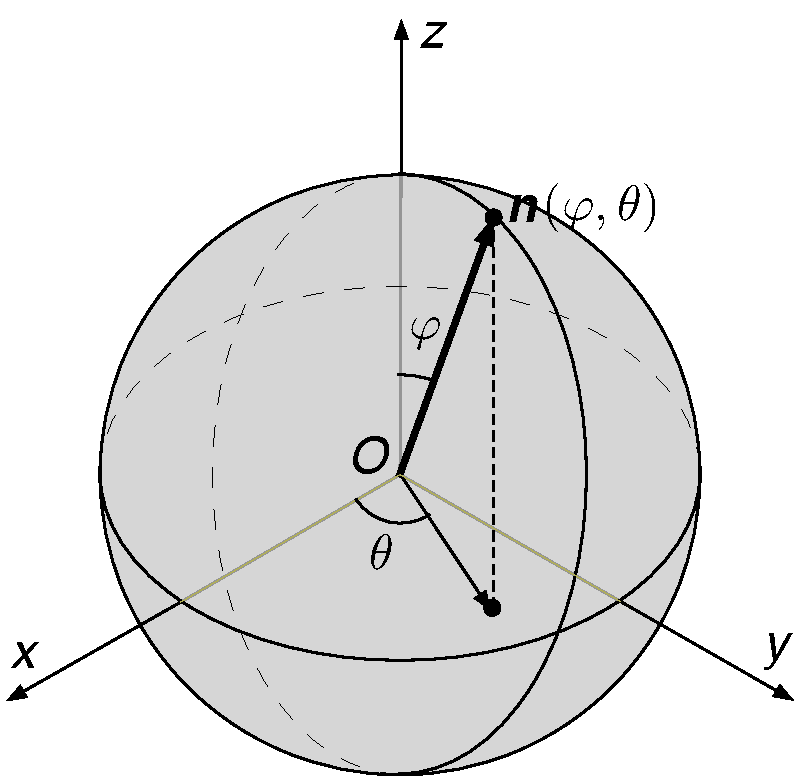
\includegraphics[width=67mm]{figs/spherical.pdf}
      \label{fig:spherical}
    }
    \subfigure[Stereographic]{
      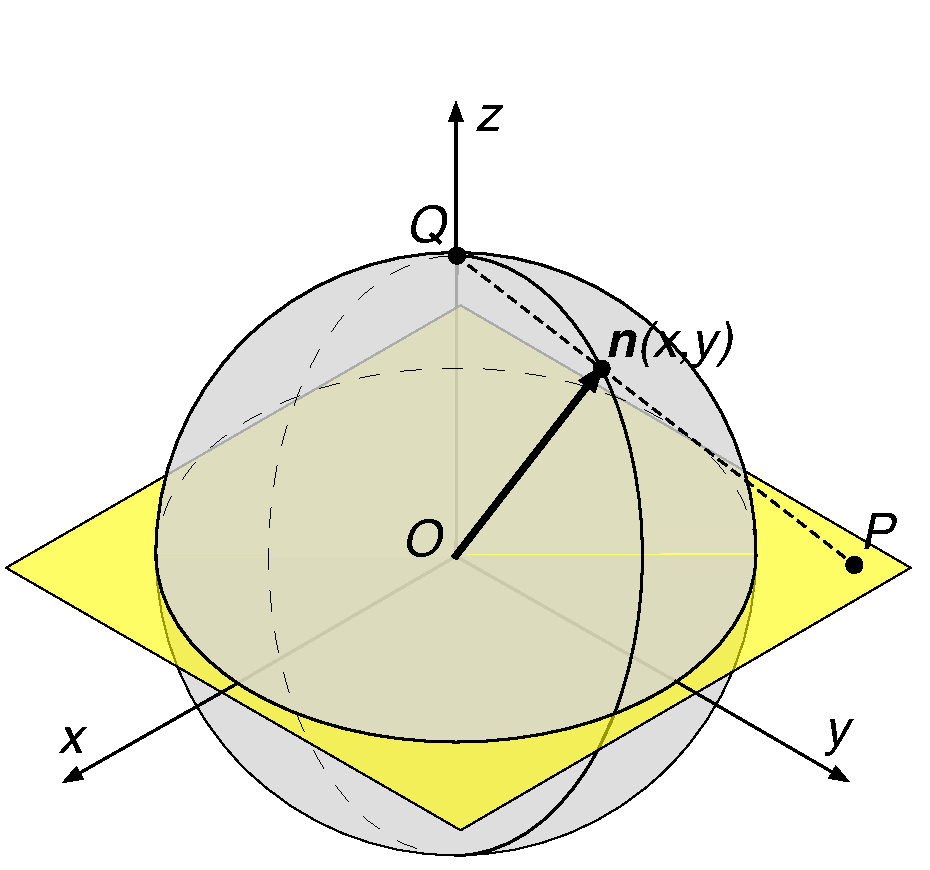
\includegraphics[width=67mm]{figs/stereographic.pdf}
      \label{fig:stereographic}
    }
    \subfigure[Projective]{
      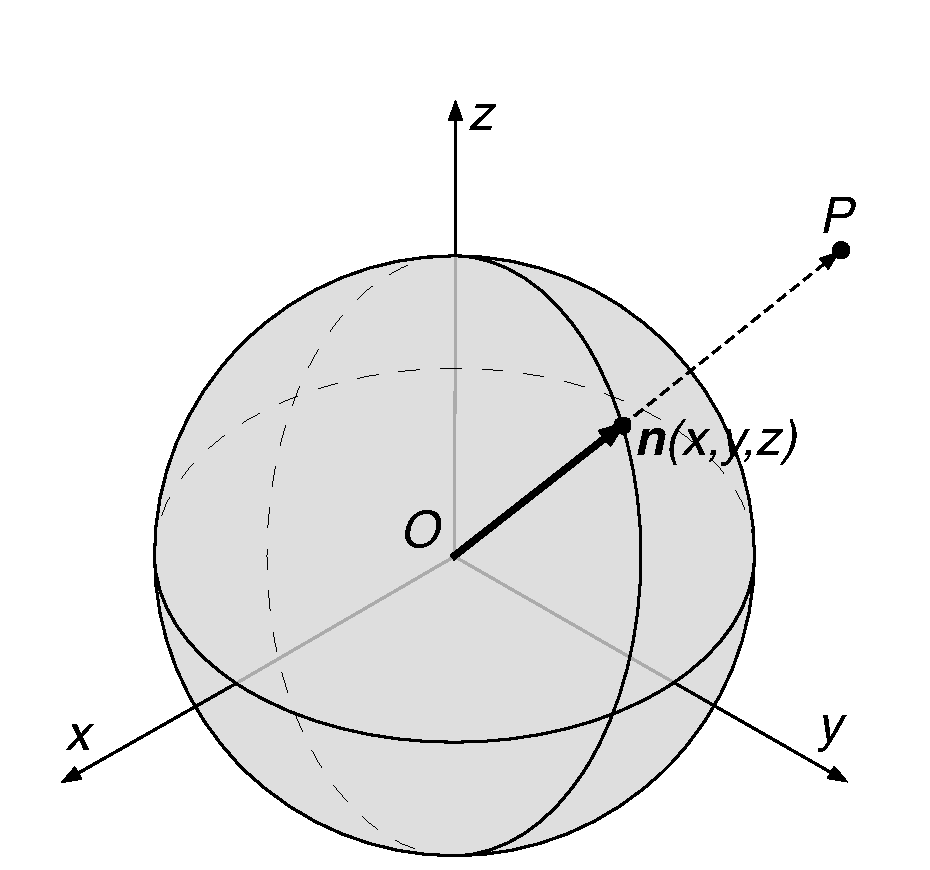
\includegraphics[width=67mm]{figs/projective.pdf}
      \label{fig:projective}
    }
    \subfigure[Tangent]{
      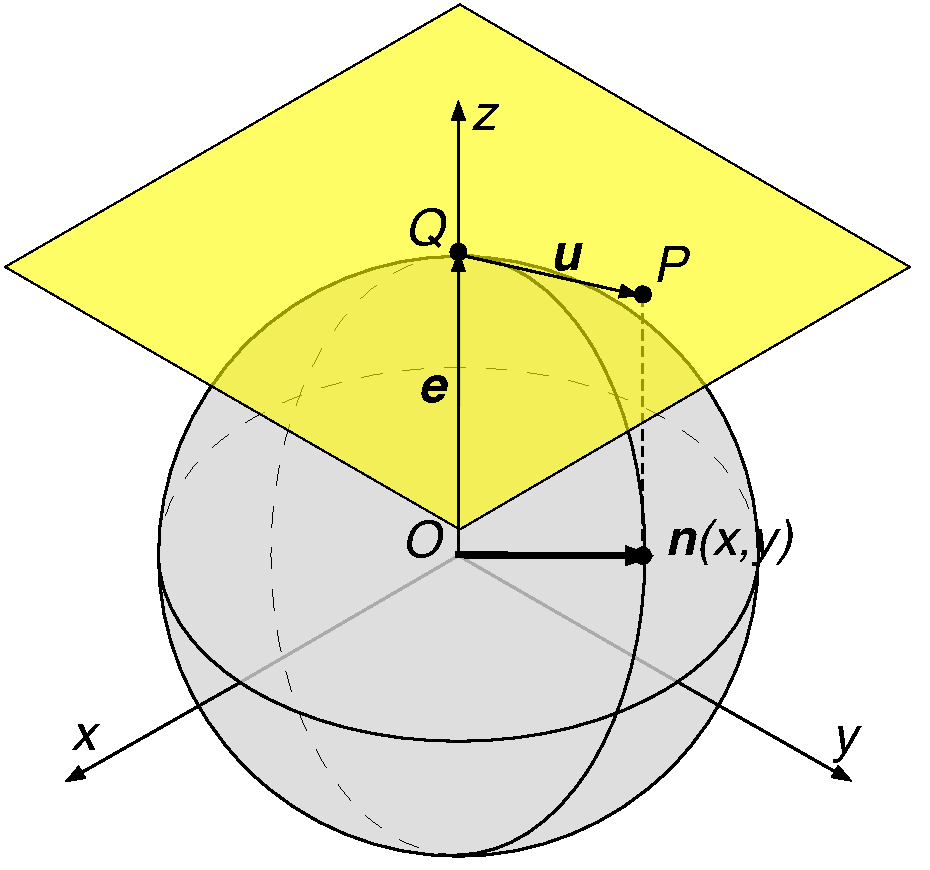
\includegraphics[width=67mm]{figs/tangent.pdf}
      \label{fig:tangent}
    }
    \subfigure[Cartesian]{
      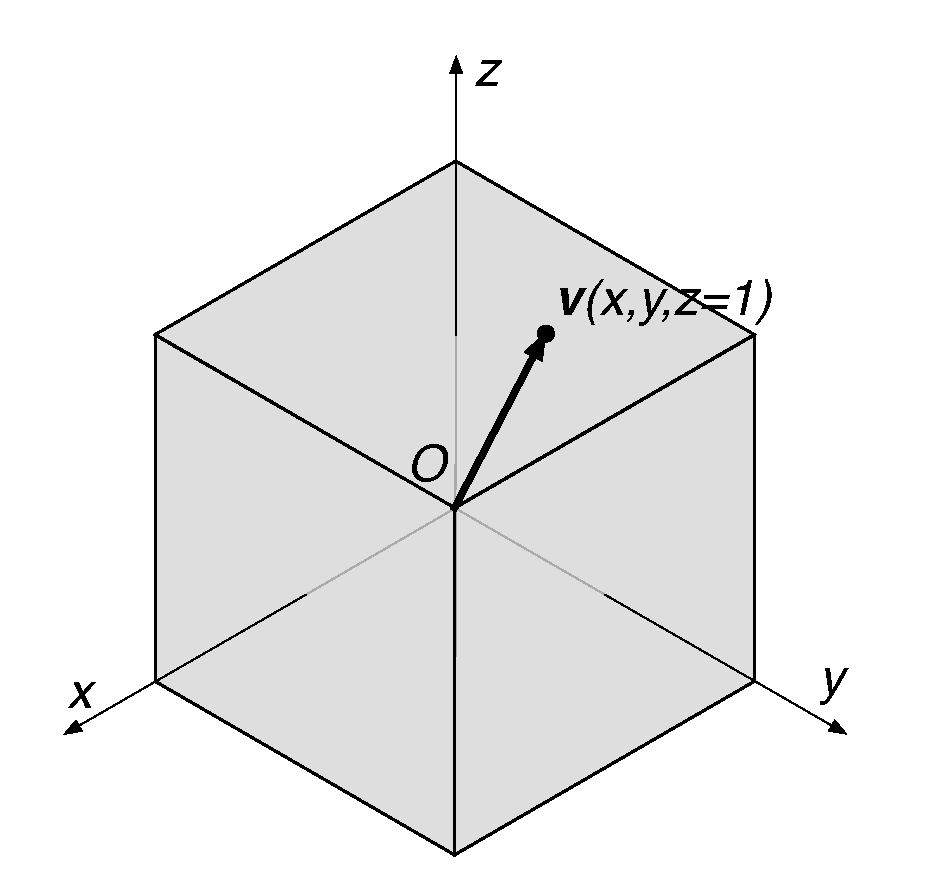
\includegraphics[width=67mm]{figs/cartesian.pdf}
      \label{fig:Cartesian}
    }
    \caption{Parametrizations.}
    \label{fig:parametrizations}
  \end{center}
\end{figure}

\section{Bifurcation Detection}
\label{sec:detection}

Within an incremental update setting, the detection of the bifurcation
condition for each time increment using any of the parametrizations
just described may be effected by the following procedure:

\begin{itemize}
  
\item An initial coarse sampling is performed over the parametric
  space for $\bq$ for the normal vector $\bn \in S^2$ or $\bv \in
  \bbR^3 \setminus \{\mathbf{0}\}$ associated with the
  parametrization. This leads to a coarse estimate of the determinant
  function $f(\bq)$.
  
\item The coarse estimate is used to initiate a Newton-type iterative
  procedure to find a better approximation to the minimum.


\end{itemize}

This simple procedure may not yield estimates of the bifurcation
condition that are accurate enough. One way to improve the solution is
to introduce adaptive time increments. Define

\begin{equation} \label{eq:general-minimization-problem}
  \mu_n := \min_{\bq} f_n(\bq) = \min_{\bq} \det \bB_n(\bq)
\end{equation}

where the tensor $\bB_n(\bq)$ may be either the one from
\eref{eq:acoustic-tensor} or the one from
\eref{eq:Cartesian-acoustic-tensor}, depending on the parametrization
in use, and the index $n$ indicates that the evaluation occurs at time
$t_n$. 

Consider the original time increment from $t_n$ to $t_{n+1}$, where 
$\mu_n > 0$ and $\mu_{n+1} < 0$. This means that between time $t_n$ 
and $t_{n+1}$, the strong ellipticity condition is violated and hence 
material bifurcates. Assume also that $\mu_n / \mu_0 > \epsilon$, 
where $\mu_0$ is the value of the determinant function evaluated at 
time $t_0$ and $\epsilon$ is a target tolerance. We wish to find a 
better estimate for the determinant function $\mu_n$, and hence the 
bifurcation time $t_n$, such that $\mu_n / \mu_0 \le \epsilon$. This 
is achieved by an adaptive time increment procedure by means of 
bisection, as shown in Algorithm~\ref{alg:adaptive-step}. This 
algorithm essentially cut the time increment to half until the 
convergence criteria $\mu_n / \mu_0 \le \epsilon$ is met.

\begin{algorithm}
  \caption{$\text{AdaptiveStep}(\mu_0, \mu_{n+1}, t_{n+1}, \epsilon)$}
  \begin{algorithmic}
    \REQUIRE $\mu_{n+1} < 0$
    \ENSURE $\mu_{n+1,k} \in [0, \epsilon \mu_0]$
    \STATE initialize
    $k \leftarrow 1,
    \quad
    \alpha \leftarrow \frac{1}{2},
    \quad
    \triangle t \leftarrow t_{n+1} - t_n,
    \quad
    \mu_{n+1,k} \leftarrow \mu_{n+1}$
    \WHILE{ $\mu_{n+1,k} < 0$ {  or  } $ \mu_{n+1,k} / \mu_0
      > \epsilon$ }
    \STATE $t_{n+1,k} \leftarrow t_n + \alpha \triangle t$
    \STATE compute $\bF(t_{n+1,k})$ using the global solution scheme
    \STATE compute $\triangle \bZ(t_{n+1,k})$
    by solving \eref{eq:Biots-equation-discrete}
    \STATE compute $\bbC(t_{n+1,k})$
    using \eref{eq:incremental-stress-moduli}
    \STATE compute $\mu_{n+1,k}$
    by solving \eref{eq:general-minimization-problem}
    \IF{$\mu_{n+1,k} > 0$}
    \STATE $\alpha \leftarrow \alpha + 2^{-k}$
    \ELSE
    \STATE $\alpha \leftarrow \alpha - 2^{-k}$
    \ENDIF
    \STATE $k \leftarrow k+1$
    \ENDWHILE
  \end{algorithmic}
  \label{alg:adaptive-step}
\end{algorithm}

The adaptive time increment procedure allows the accurate (up to the
tolerance $\epsilon$) detection of bifurcation time during a loading
process.

\section{Numerical Examples}
\label{sec:numerical-examples}

The performance and applicability of the parametrizations described in
Section~\ref{sec:parametrizations} are examined by applying them to 
the bifurcation analysis of several material models under different 
loading conditions. The analysis is performed at the material point 
level. Of particular interest are the robustness and computational 
efficiency of different parametrizations.

\subsection{Small deformation isotropic elastic damage model}
\label{subsec:isotropic}

We start the bifurcation analysis on a simple small deformation 
isotropic damage model. The model formulation is briefly presented 
first. Then, a simple shear test will be performed to study the 
performance of different parametrizations on the detection of material 
bifurcation.

\subsubsection{Model formulation}
The stress and constitutive tangent of the small deformation isotropic 
damage model will be derived from a strain-energy function, which is 
assumed to have the following form:

\begin{equation}\label{eq:iso_psi}
 \Psi(\bepsilon ^e, \xi)
   = \frac{1}{2} (1 - \xi) 
     \bepsilon ^e : \mathbb{C}^e : \bepsilon ^e
\end{equation}

where $\bepsilon^e$ is the infinitesimal elastic strain tensor, 
$\mathbb{C}^e$ is the fourth-order elastic modulus, and $\xi$ 
is a damage parameter introduced to trigger material bifurcation. For 
isotropic linear elasticity, the elastic modulus $\mathbb{C}^e$ is 
given as

\begin{equation}
  \mathbb{C}^e = \lambda \bdelta\otimes\delta + 2\mu\bI
\end{equation}

where $\lambda$ and $\mu$ are Lam\'{e} constant and shear modulus,
respectively. $\bdelta$ is the second-order identity tensor,
$(\bI)_{ijkl} = 1/2(\delta_{ik}\delta_{jl} +
\delta_{il}\delta_{jk})$ is the fourth-order symmetric identity
tensor.

We adopt the following evolution law for the scalar damage parameter $
\xi$ \cite{Holzapfel:2000}

\begin{equation}\label{eq:iso_xi}
  \xi(\alpha) = \xi_{\infty} [ 1- {\rm exp}(-\alpha / \tau)]
\end{equation}

where $\xi_{\infty}$ describes the dimensionless maximum damage and
$\tau$ is referred to as the damage saturation parameter. $s \in
[0,t]$ denotes the history variable. The parameter $\alpha$ is the
maximum thermodynamic force \cite{Holzapfel:2000}

\begin{equation}
  \alpha(t) = \max_{s\in [0,t]}\Psi_0(s)
\end{equation}

where $\Psi_0(s)$ is the undamaged strain energy at time $s$.

Given the strain-energy function \eref{eq:iso_psi} and the damage
evolution \eref{eq:iso_xi}, the fourth-order tangent modulus can be
derived by taking 2nd derivative of the strain-energy function with
respect to strain measure $\bepsilon_e$, which results in

\begin{equation}
  \mathbb{C} = (1-\xi)\mathbb{C}^e 
    - \beta \frac{\partial\xi}{\partial\alpha}
    (\bsigma_0\otimes\bsigma_0)
\end{equation}

where $\beta = 1$ if damage evolves within the time increment and 
$\beta=0$ otherwise. This tangent modulus will be used to compute the 
acoustic tensor \eref{eq:acoustic-tensor}, which will then be checked 
for material bifurcation.

\subsubsection{Simple shear test}

The above small deformation material model is loaded under a simple 
shear condition, where the following material properties are used:
$\lambda = 80$, $\mu = 80$, $\xi_{\infty} = 1.0$ and $\tau = 1.0$. The 
resulting shear stress vs. shear strain is plotted in Figure 
\ref{fig:iso_stress_strain}(a). The softening response is due to the 
evolution of the introduced damage parameter $\xi$. 

For the detection of material bifurcation, the two-step procedure 
described in Section \ref{sec:detection} is adopted, i.e., (1) an 
initial sampling performed over the parametric space, and (2) a 
Newton-type iterative procedure for better estimation of the minimum 
det$\bA$. Figure \ref{fig:iso_stress_strain}(b) shows the degradation 
of the determinant function det$\bA$ for all five 
parametrizations. When det$\bA = 0$, the material bifurcates. In 
this example, all five parametrizations detect bifurcation at the same 
time, i.e., when the shear strain $\bepsilon_{12}=0.0559$ as marked in 
Figure \ref{fig:iso_stress_strain}(a). With the adaptive time step 
algorithm, the precise time (upto the set tolerance) of bifurcation 
can be detected.

\begin{figure}[H]
  \centering \subfigure[]{
    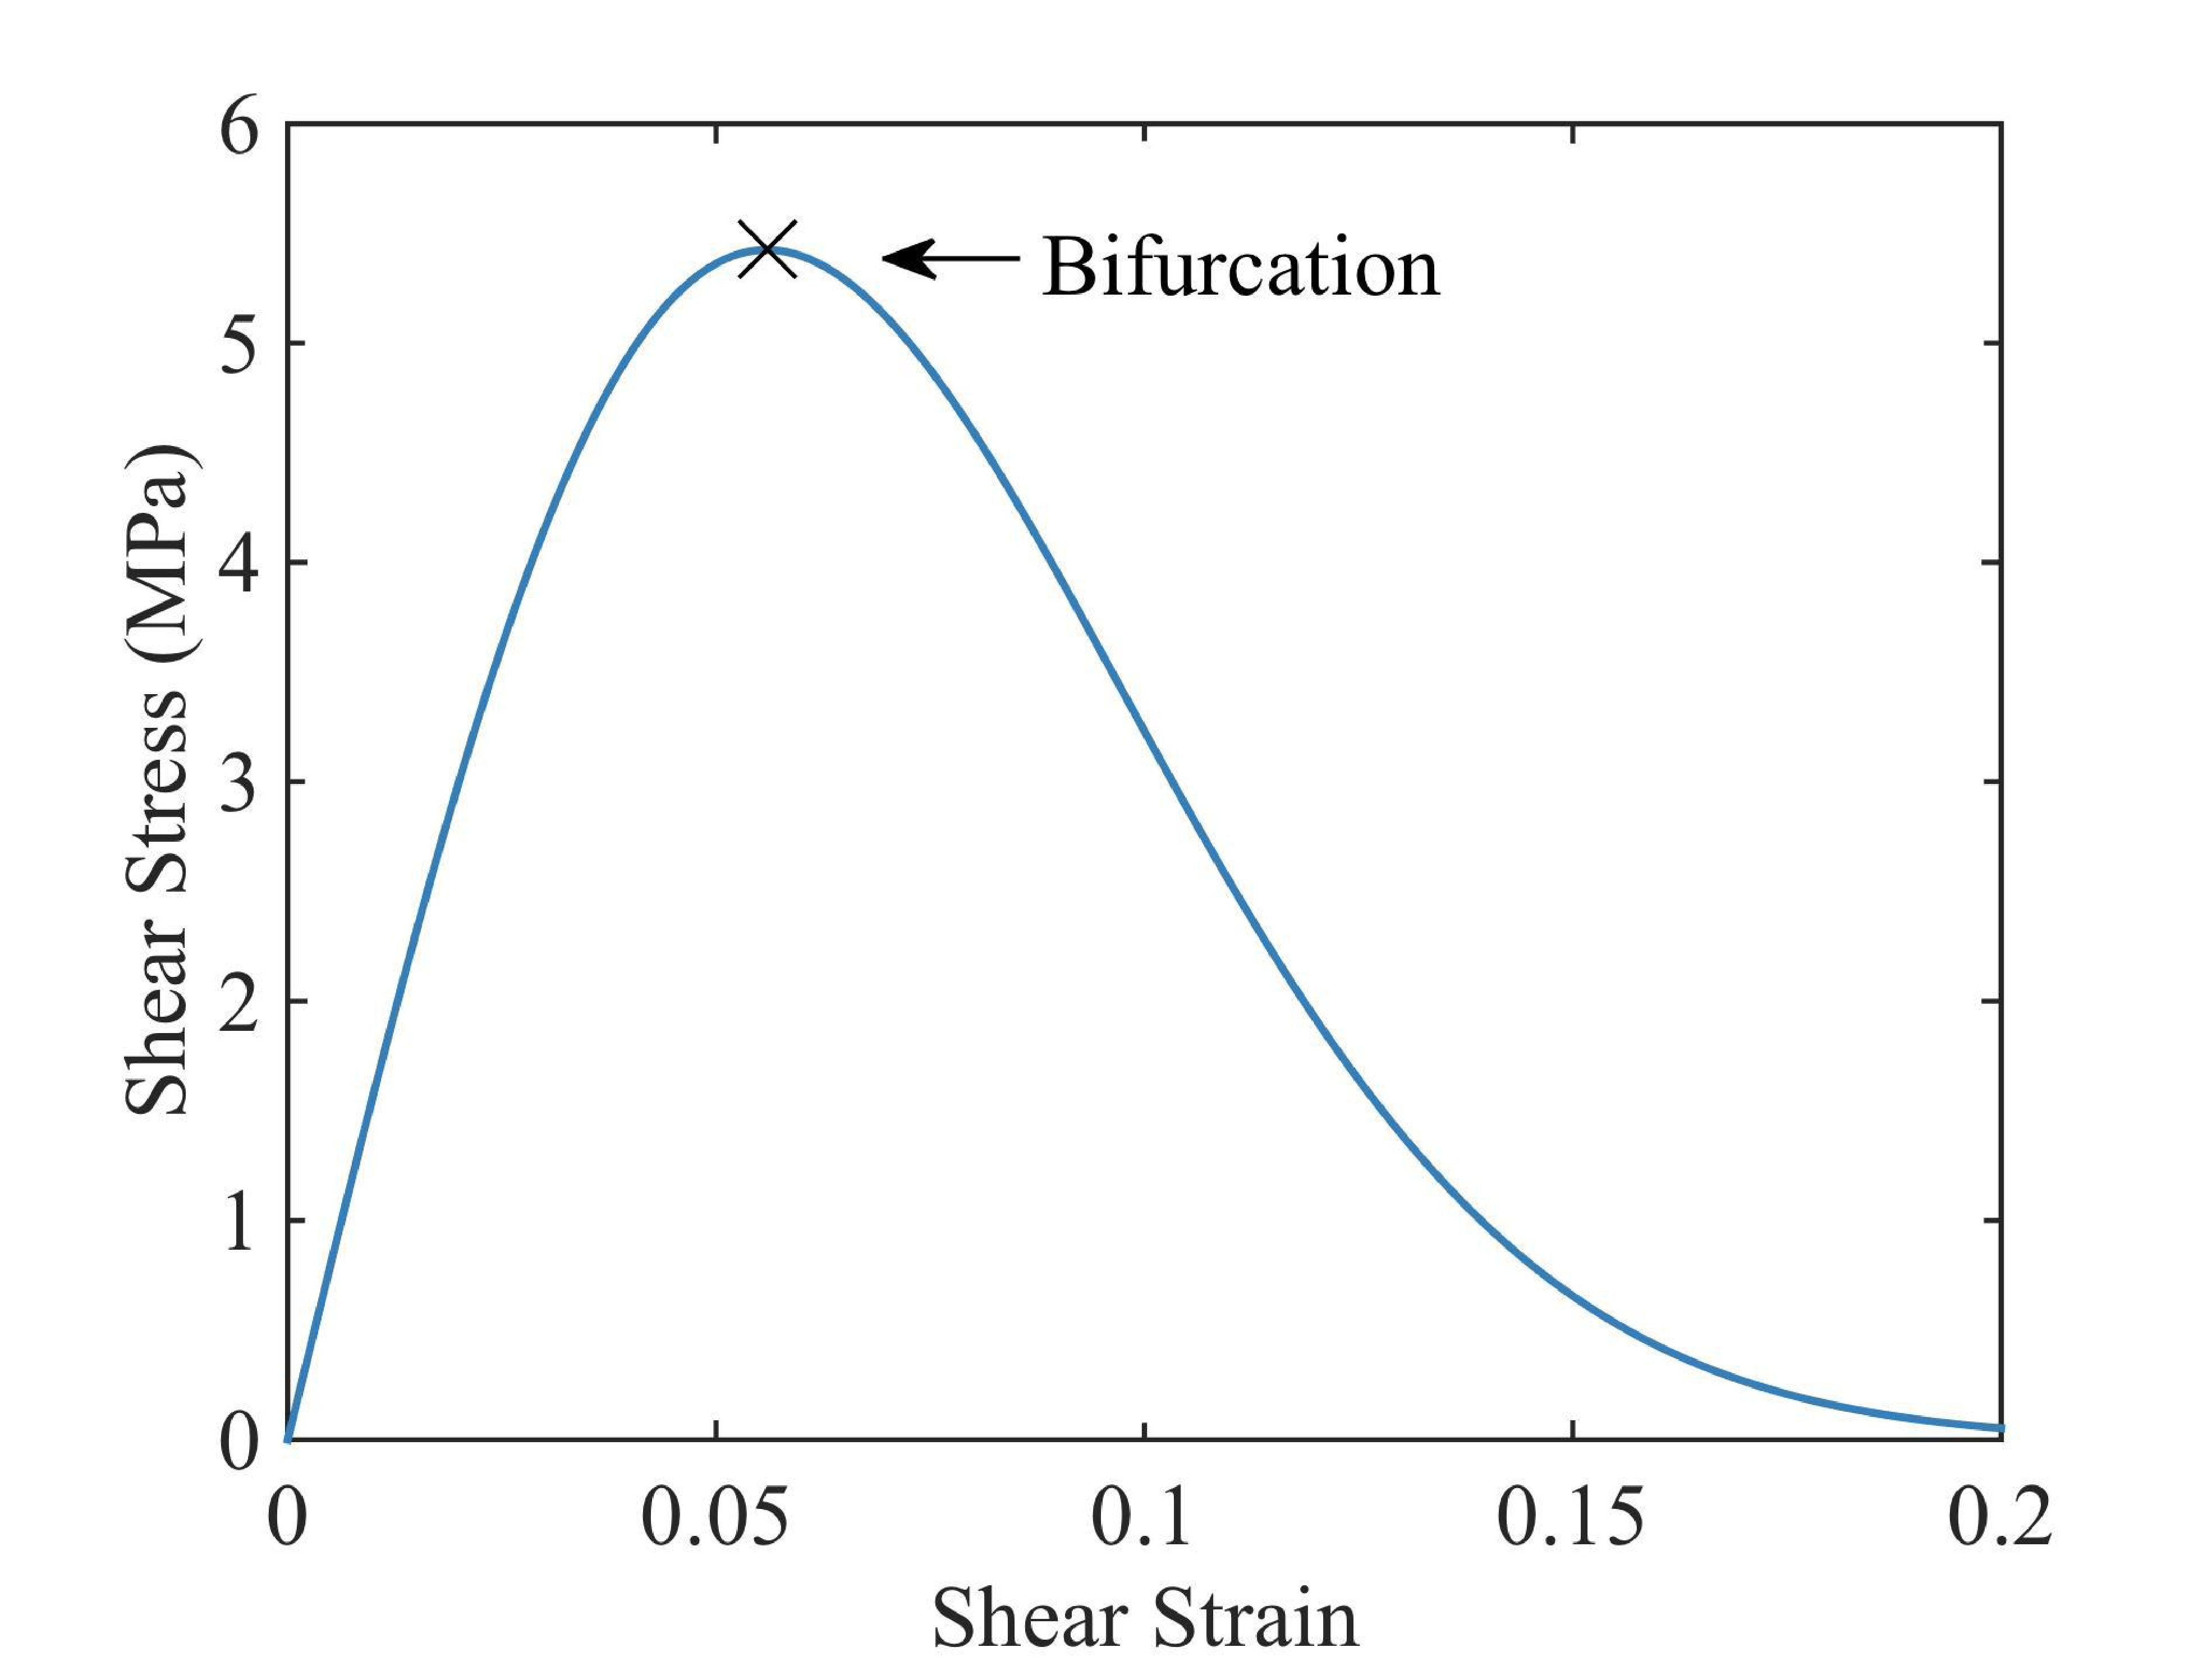
\includegraphics[width=0.45\textwidth]
    {figs/iso_shear_stress_strain.pdf}
  } \subfigure[]{
    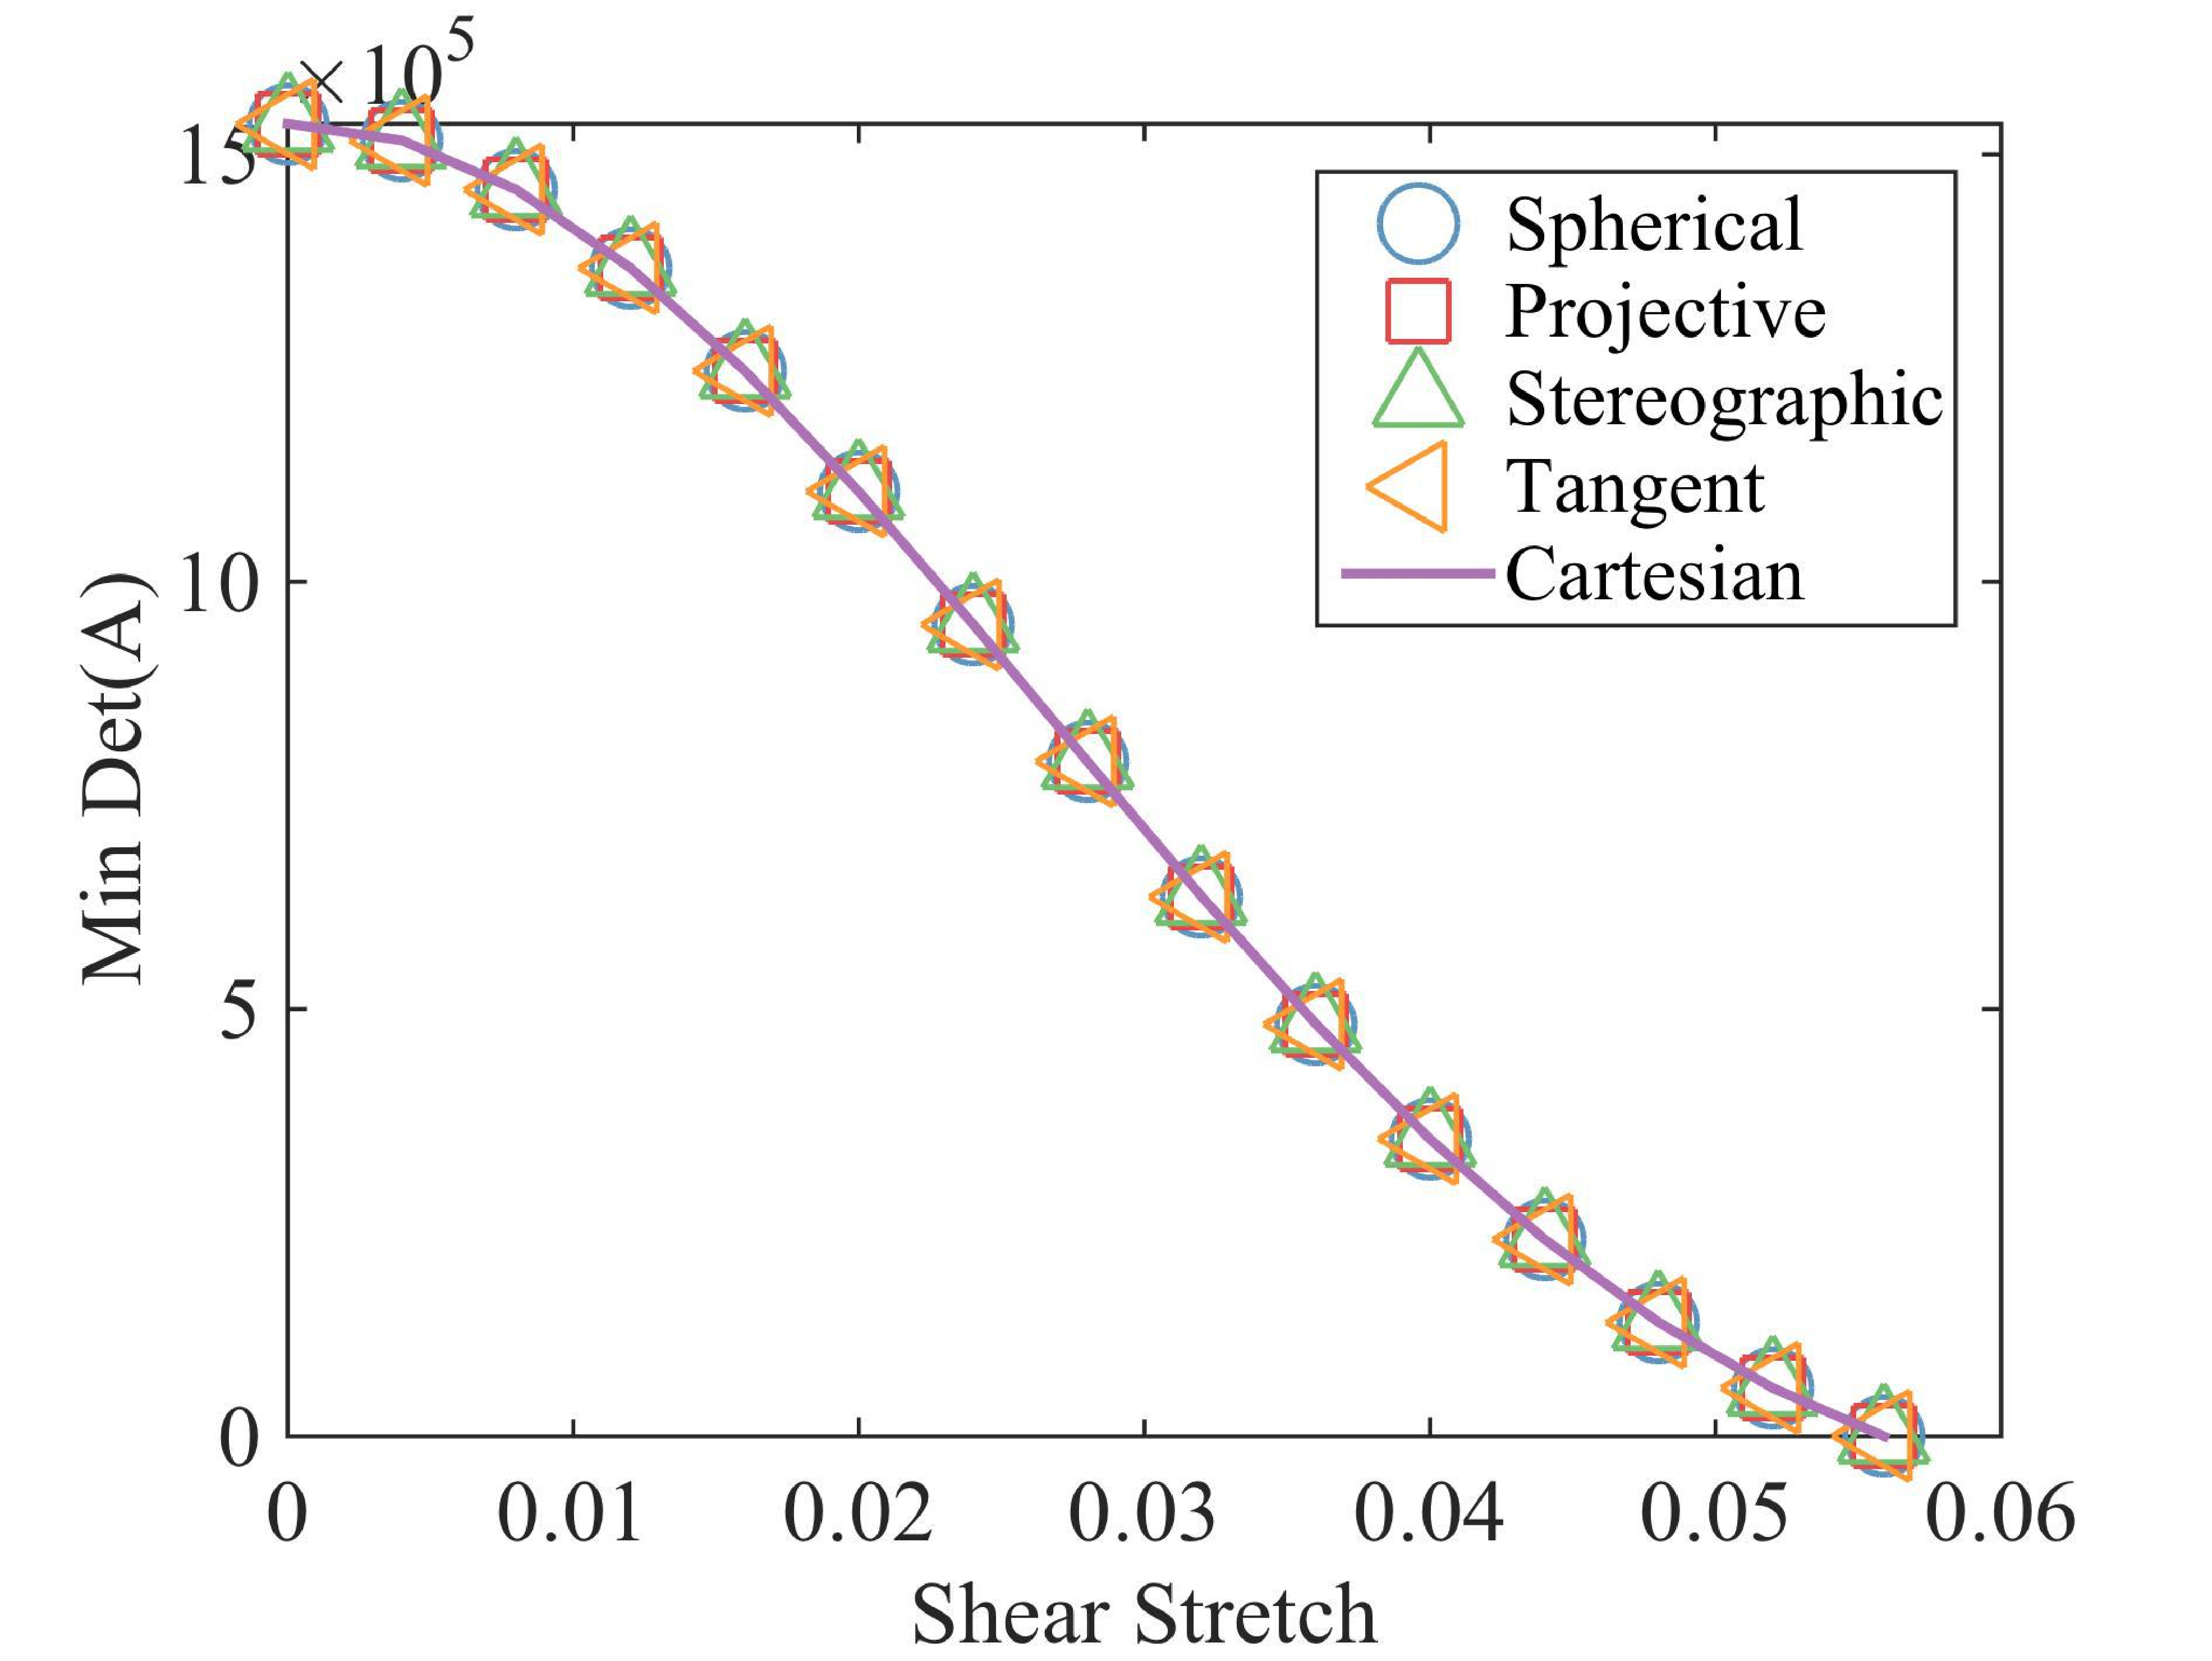
\includegraphics[width=0.45\textwidth]
    {figs/iso_shear_mindetA_strain.pdf}
  }
  \caption{Simple shear test on small deformation 
  isotropic damage model: 
  (a)stress strain behavior, with red cross indicating bifurcation, and
  (b) degradation of det$\bA$ for different
  parametrizations.}
  \label{fig:iso_stress_strain}
\end{figure}

While all five parametrizations detect bifurcation at the same time, 
Figure \ref{fig:iso_stress_strain}(b) provides little information on 
their computational efficiency and robustness, which are the focus of 
this work. The computational cost of bifurcation detection mainly 
consists of two parts: (1) the time for the initial sampling over the 
parametric space, and (2) the time for the Newton-type iterative 
solve. 

The time for the initial sampling depends on the number of sampling 
points, or equivalently, the density of the initial sampling grid. The 
denser the initial sampling grid is, the more expensive it is 
computationally to perform the sweep. The time for the Newton-type 
iterative solve depends mainly on the complexity of the objective 
function, i.e., det$\bA$, as well as the quality of the initial guess.

To compare computational costs of different parametrizations, we 
record the time spent on bifurcation check at a particular loading 
increment, e.g., at the increment leading to bifurcation. For 
robustness, we will change the density of initial sampling grids and 
study the effect of this change on the detection of bifurcation using 
different parametrizations. A robust parametrization should be 
relatively insensitive to the density of the initial sampling grids.

The results on computational cost and robustness are summarized in 
Table \ref{tab:iso_shear_runtime}. The density of the initial 
sampling grid is represented by the sampling interval and the number 
of sampling points. The table only shows the number of sampling 
points, $N$, along one dimension of the parametric space. The total 
number of sampling points should be the $N^{dim}$, where $dim$ is the 
total dimension of the parametric space. For instance, for spherical 
parametrization, there are two independent parameters, $\varphi$ and $
\theta$. Therefore, $dim=2$ for spherical parametrization.

It can be seen from Table \ref{tab:iso_shear_runtime}, as the number 
of sampling points $N$ per dimension decreases, so does the 
computational cost. The spherical and the Cartesian parametrizations 
are the most efficient and robust. The stereographic, projective and 
tangent are more expensive. In the extreme case with $N=1$, meaning 
there is only one initial sampling point per dimension, the 
stereographic, projective and tangent fail to correctly detect 
bifurcation, shown as `n/a' in the table. 

\begin{table}[H]
  \begin{center}
    %\begin{tabular}{ p{1.5cm} | p{1.7cm} p{1.7cm} p{1.7cm} p{1.7cm} p{1.7cm} }
    \begin{tabular}{c c | r r r r r}
      \toprule
      Sampling   & Sampling &   \multicolumn{5}{c}{Run time ($\mu$s)}	\\   
      interval     & points ($N$)     &  Spherical    &   Stereographic  &   Projective  &   Tangent   & Cartesian  \\
      \midrule         
      0.05      &      41     &    340        &       188       &       5458      &      225       &       401         \\
      0.1        &      21     &    152        &       92         &       909        &      123       &       162         \\
      0.2        &      11     &    87          &       69         &       218        &      91         &       100         \\
      0.3        &      7       &    83          &       201       &       216        &      221       &       81          \\
      0.4        &      5       &    83          &       232       &       242        &      185       &       71          \\       
      0.5        &	    5       &    75          &       63         &       143        &      80         &       71          \\
      0.6        &	    3       &    76          &       251       &       221        &      282       &       66          \\
      0.7        &	    3       &    76	      &       203       &       242        &      260       &       66          \\
      0.8        &      3       &    76          &       204       &       246        &      177       &       65          \\	      
      0.9        &	    3       &    76          &       207       &       194        &      272       &       69          \\	
      1.0        &      3	     &    66	      &       76         &       166        &      76         &       67          \\	
      1.5        &	    1       &    75	      &       n/a        &       n/a         &      n/a        &       66          \\	       
      \bottomrule
    \end{tabular}
    \caption{Computational cost of different parametrizations in 
    simple shear test at loading increment leading to bifurcation. 
    `n/a' means the parametrization fails to detect bifurcation in 
    this loading increment.}
    \label{tab:iso_shear_runtime}
  \end{center}
\end{table}

As aforementioned, the choice of parametrization directly affects the 
complexity of the objective function ${\rm det}\bA$ in 
\eref{eq:minimization-derivative}, which in turn affects the 
computational efficiency and robustness of different parametrizations 
on detection of material bifurcation as shown in 
Table \ref{tab:iso_shear_runtime}. To illustrate this point, the 
landscapes of the objective function ${\rm det}\bA$ at bifurcation, 
i.e., at $\bepsilon_{12}=0.0559$ are plotted in 
Figure  \ref{fig:iso_shear_detA}. The corresponding plane views of the 
determinant landscapes are shown in 
Figure \ref{fig:iso_shear_detAXplane}, where the white stars indicate 
global minimum point(s). The projective parametrization requires three parameters and is not visualized in this work.

From the landscape plots, it is clear that the complexity of the 
determinant function depends greatly on the choices of 
parametrization. Even for a very simple small deformation isotropic 
model adopted in this example, the landscape of the determinant 
function can be quite complicated in certain parametrizations, e.g., 
the stereographic and tangent ones. 

The cartesian parametrization results in a simple `bowl-shaped' 
objective function, which makes the Newton-type iterative solve 
particularly robust and insensitive to the initial guess. This has 
been reflected in Table \ref{tab:iso_shear_runtime}, where the 
cartesian parametrization is able to correctly detect bifurcation even 
with very few initial sampling point. 

\begin{figure}[H]
   \centering \subfigure[Spherical]{
   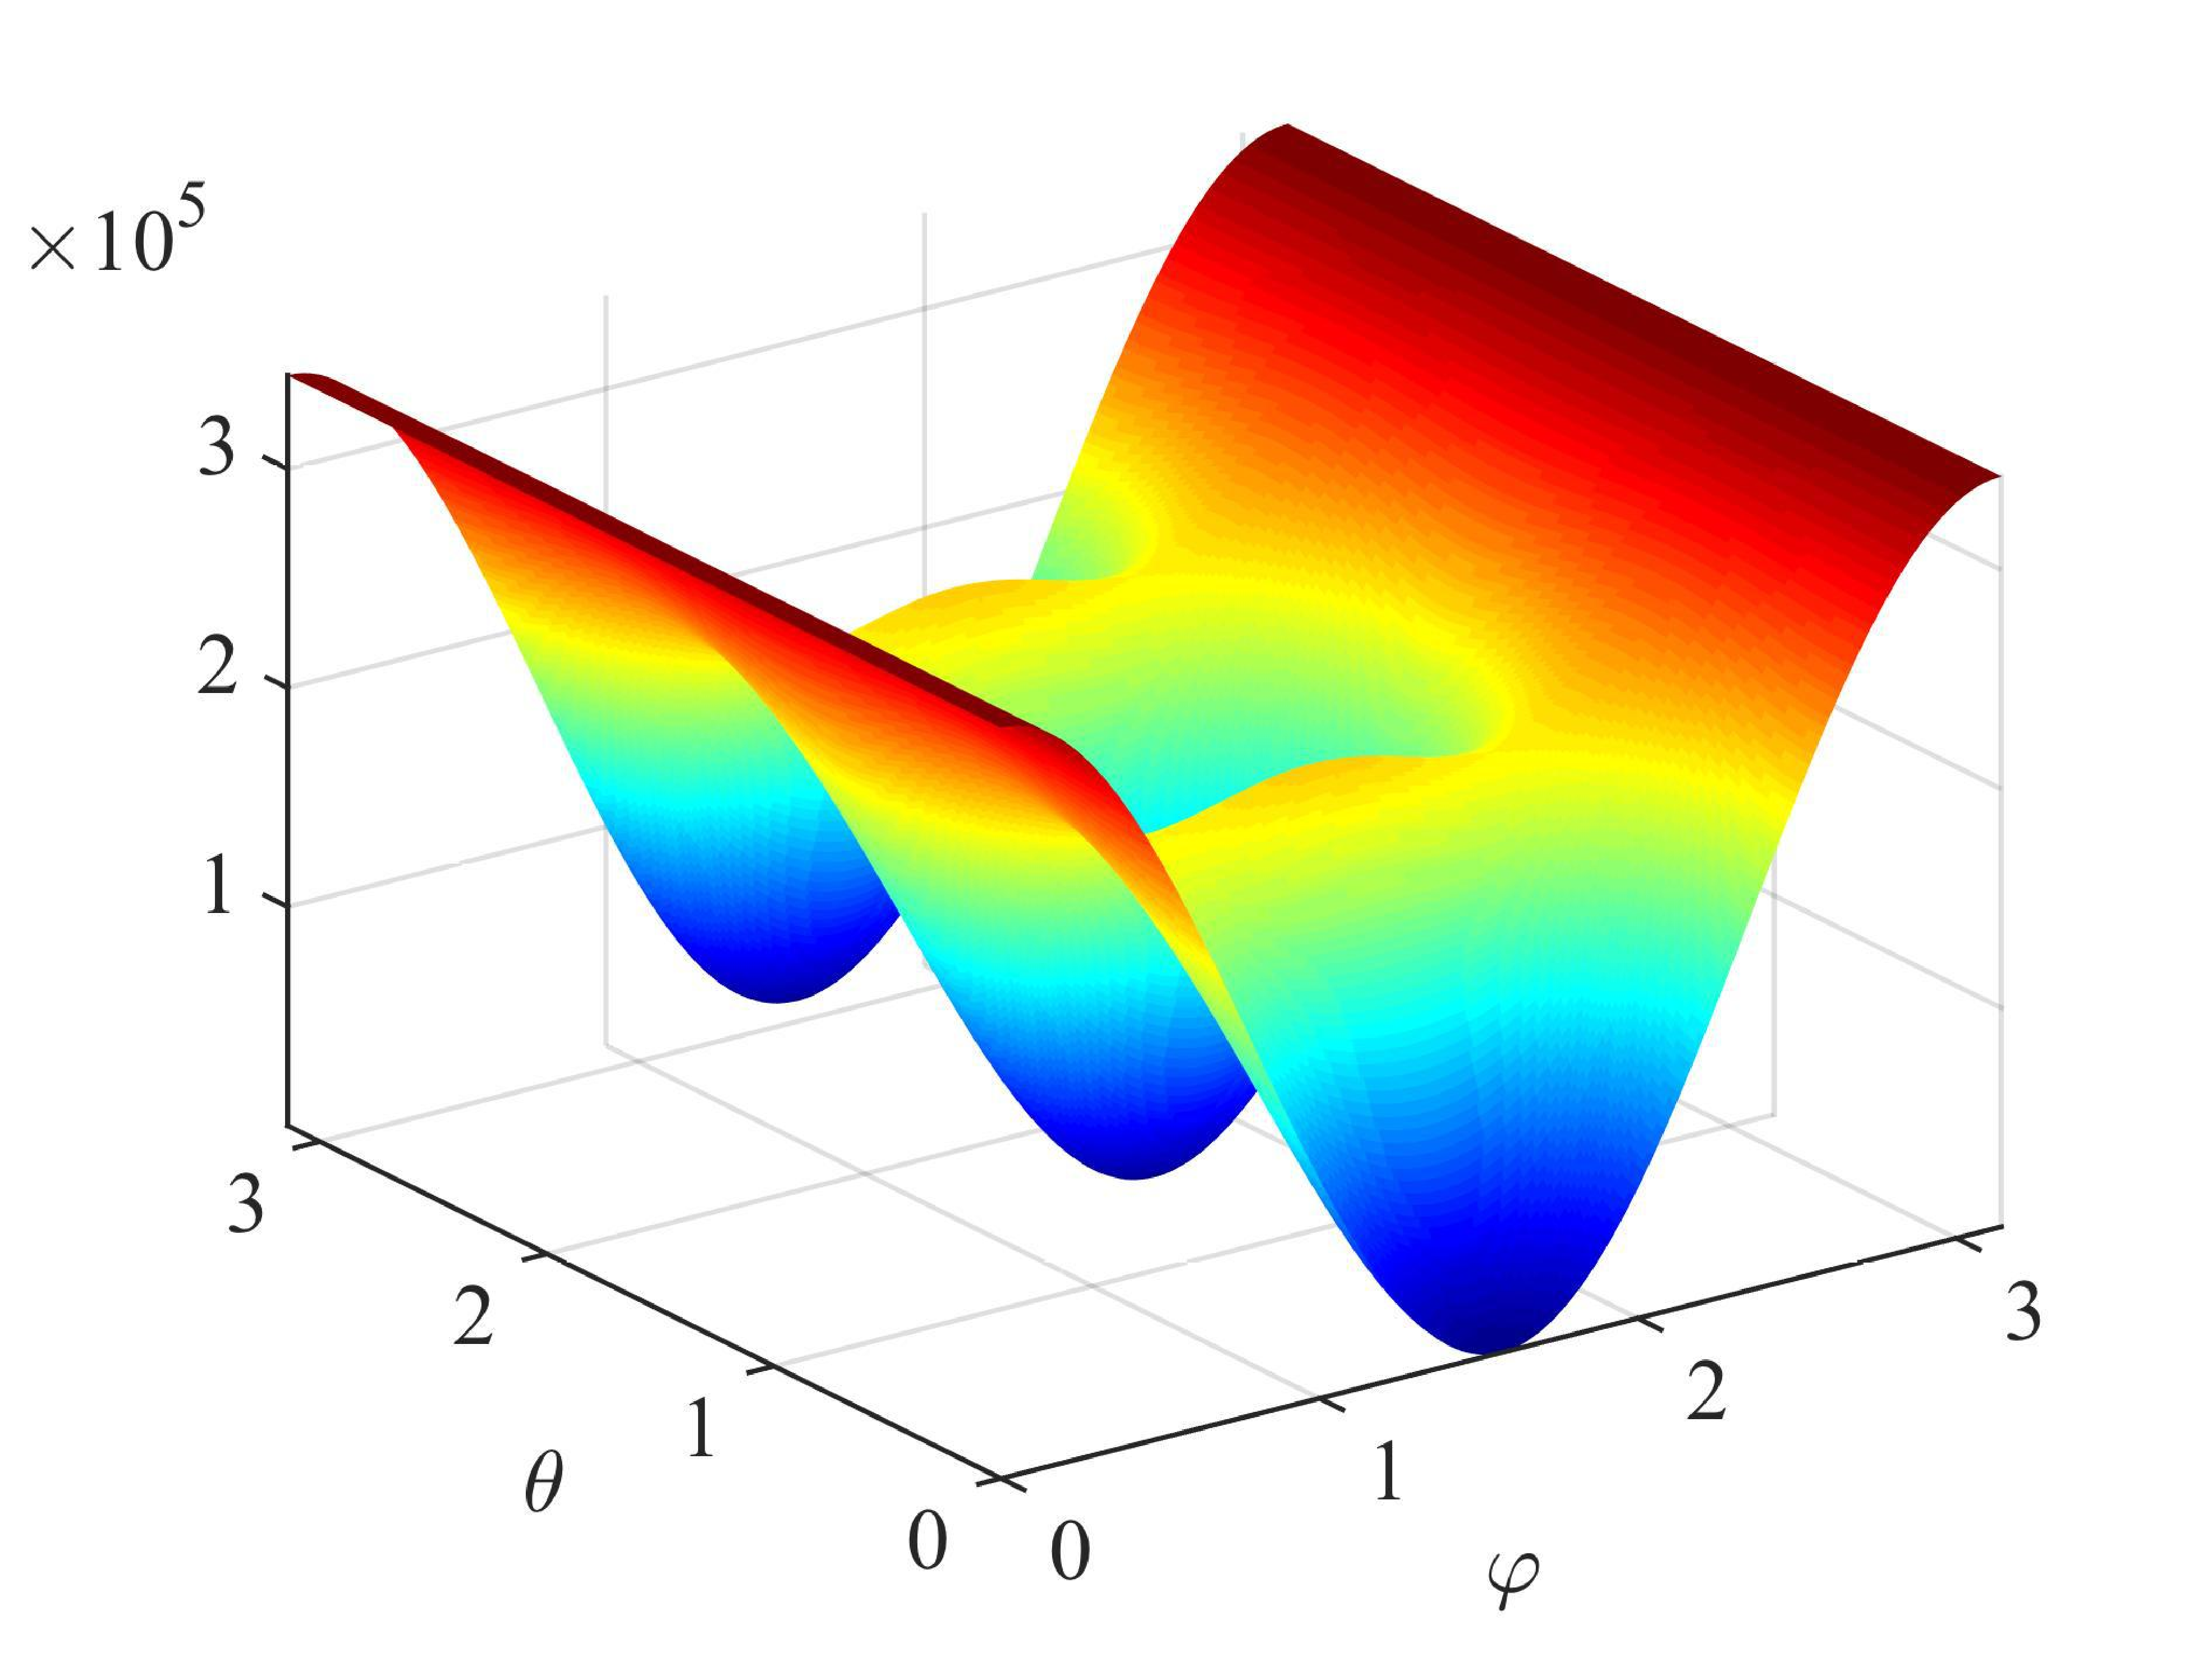
\includegraphics[width=0.45\textwidth]
   {figs/iso_shear_spherical_detA.pdf}
 } \subfigure[Cartesian]{
   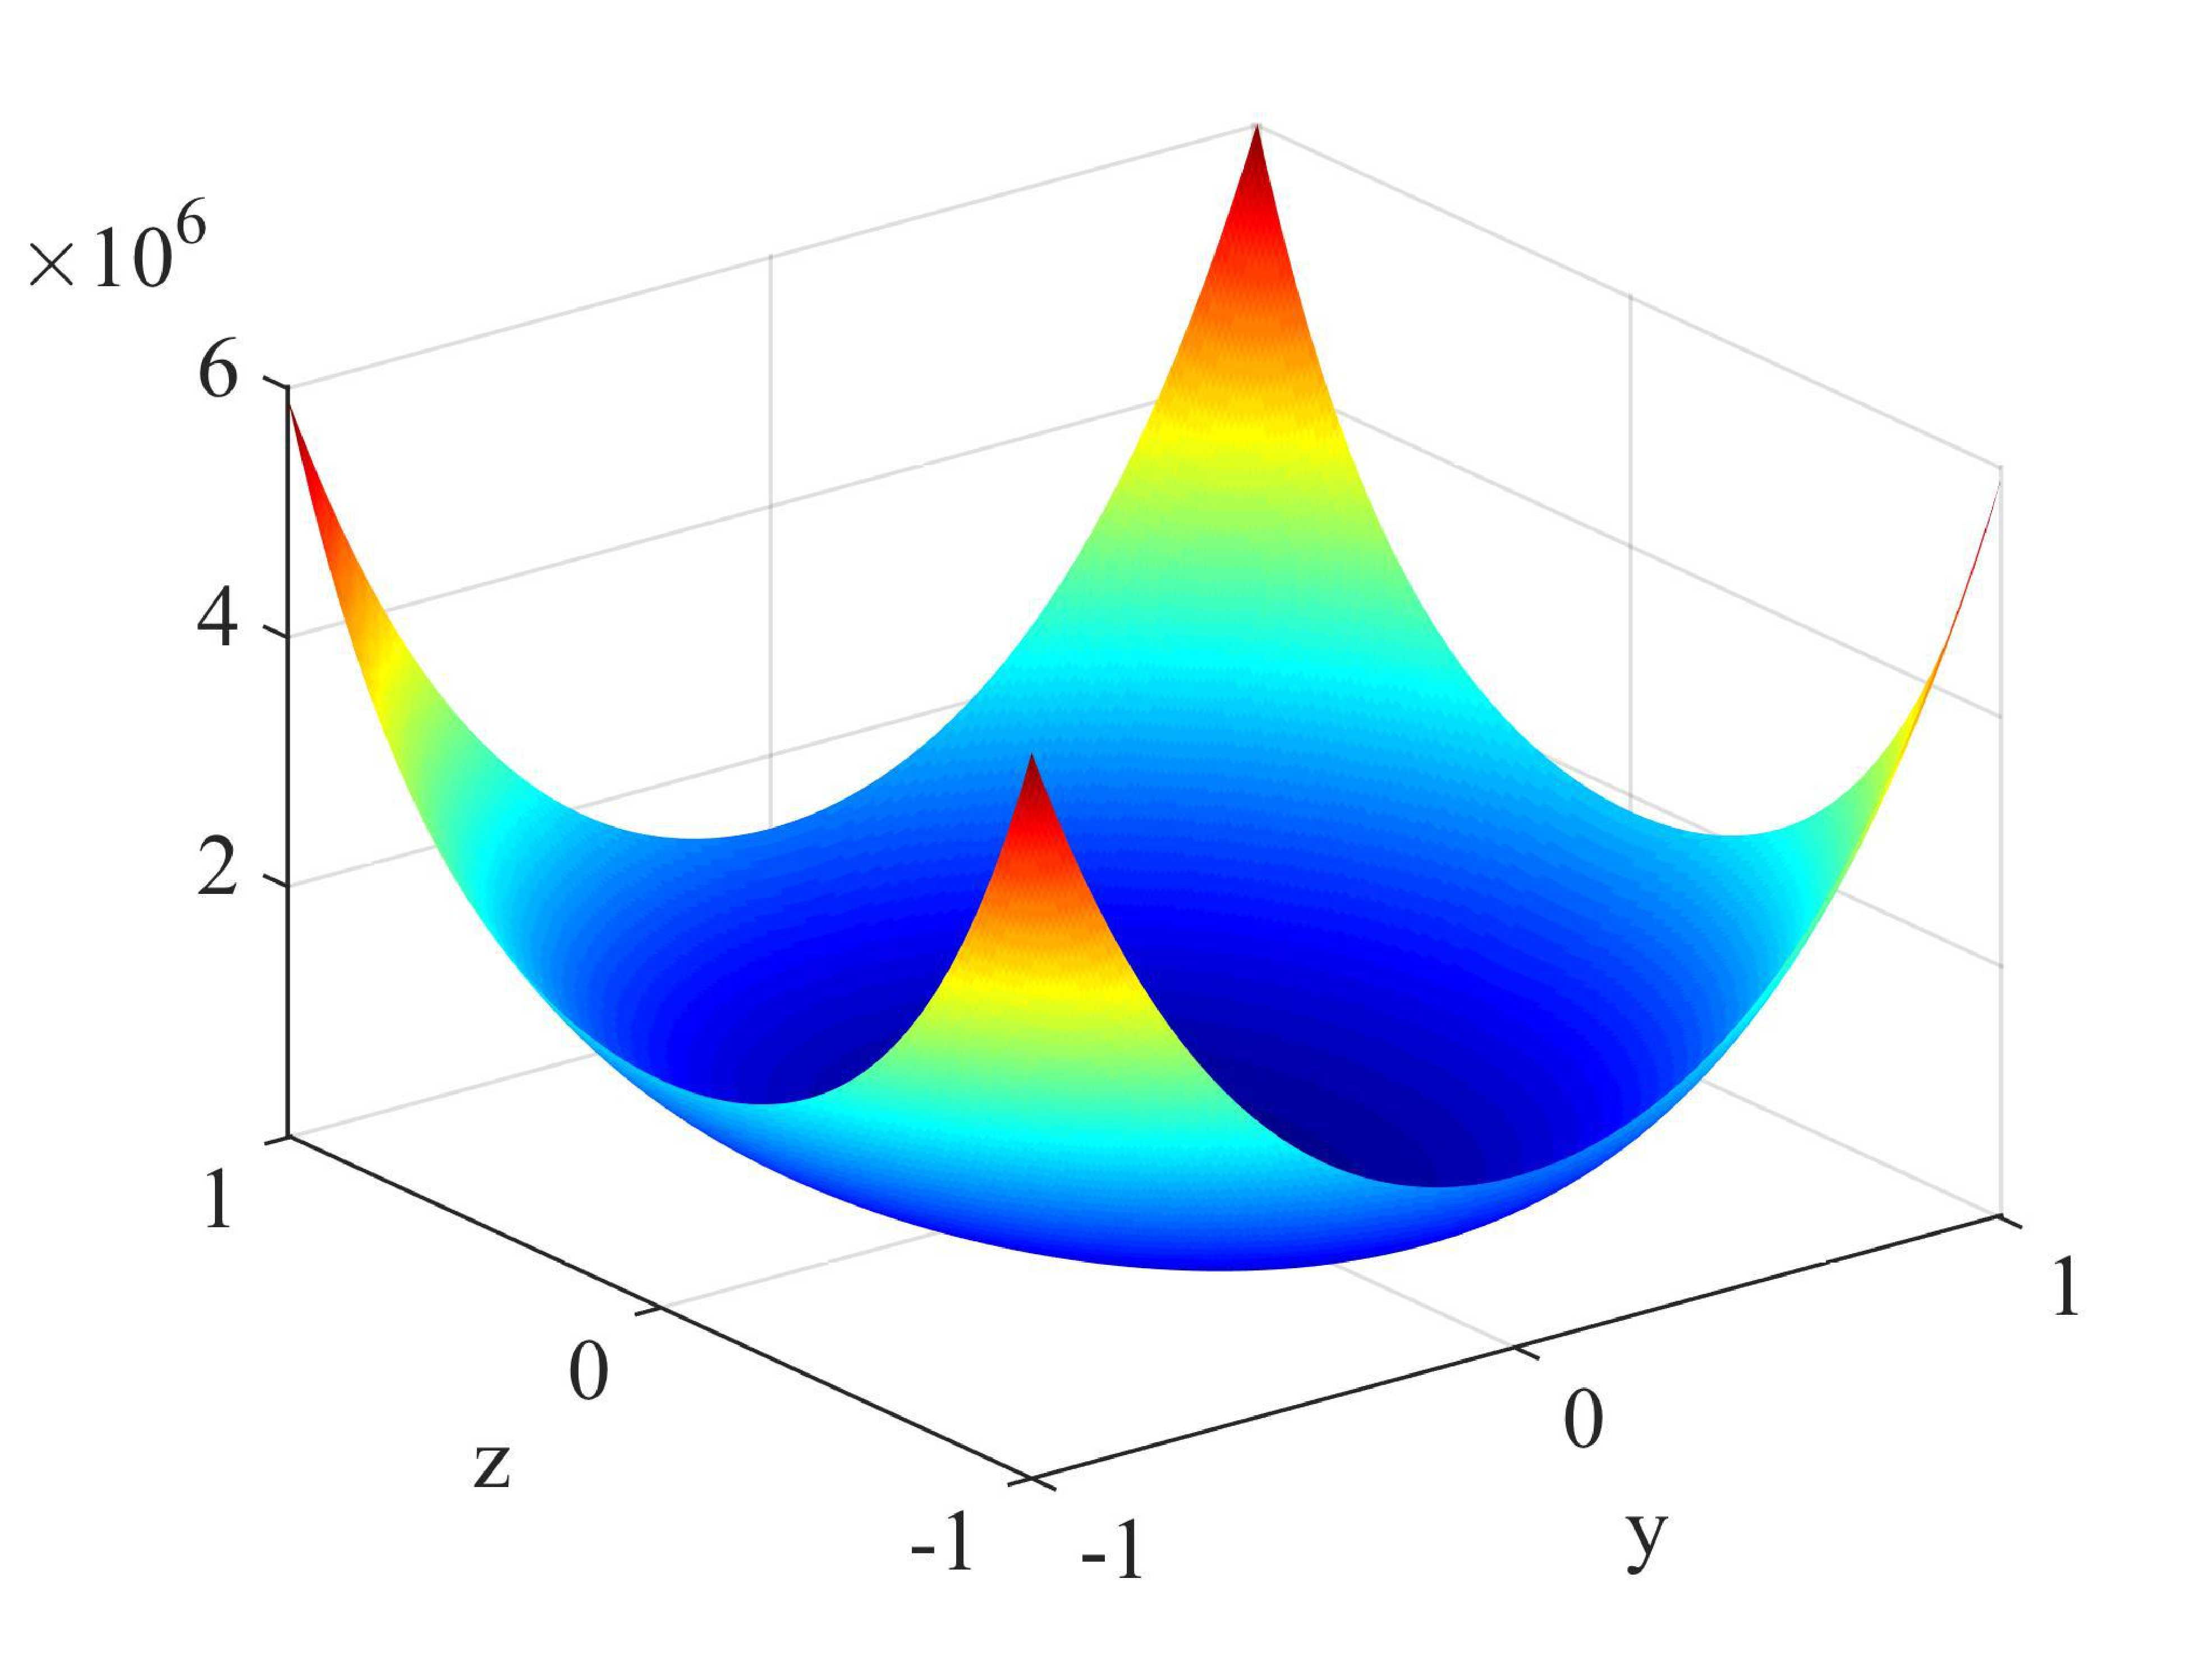
\includegraphics[width=0.45\textwidth]
   {figs/iso_shear_cartesian_detA.pdf}
 } \subfigure[Stereographic]{
   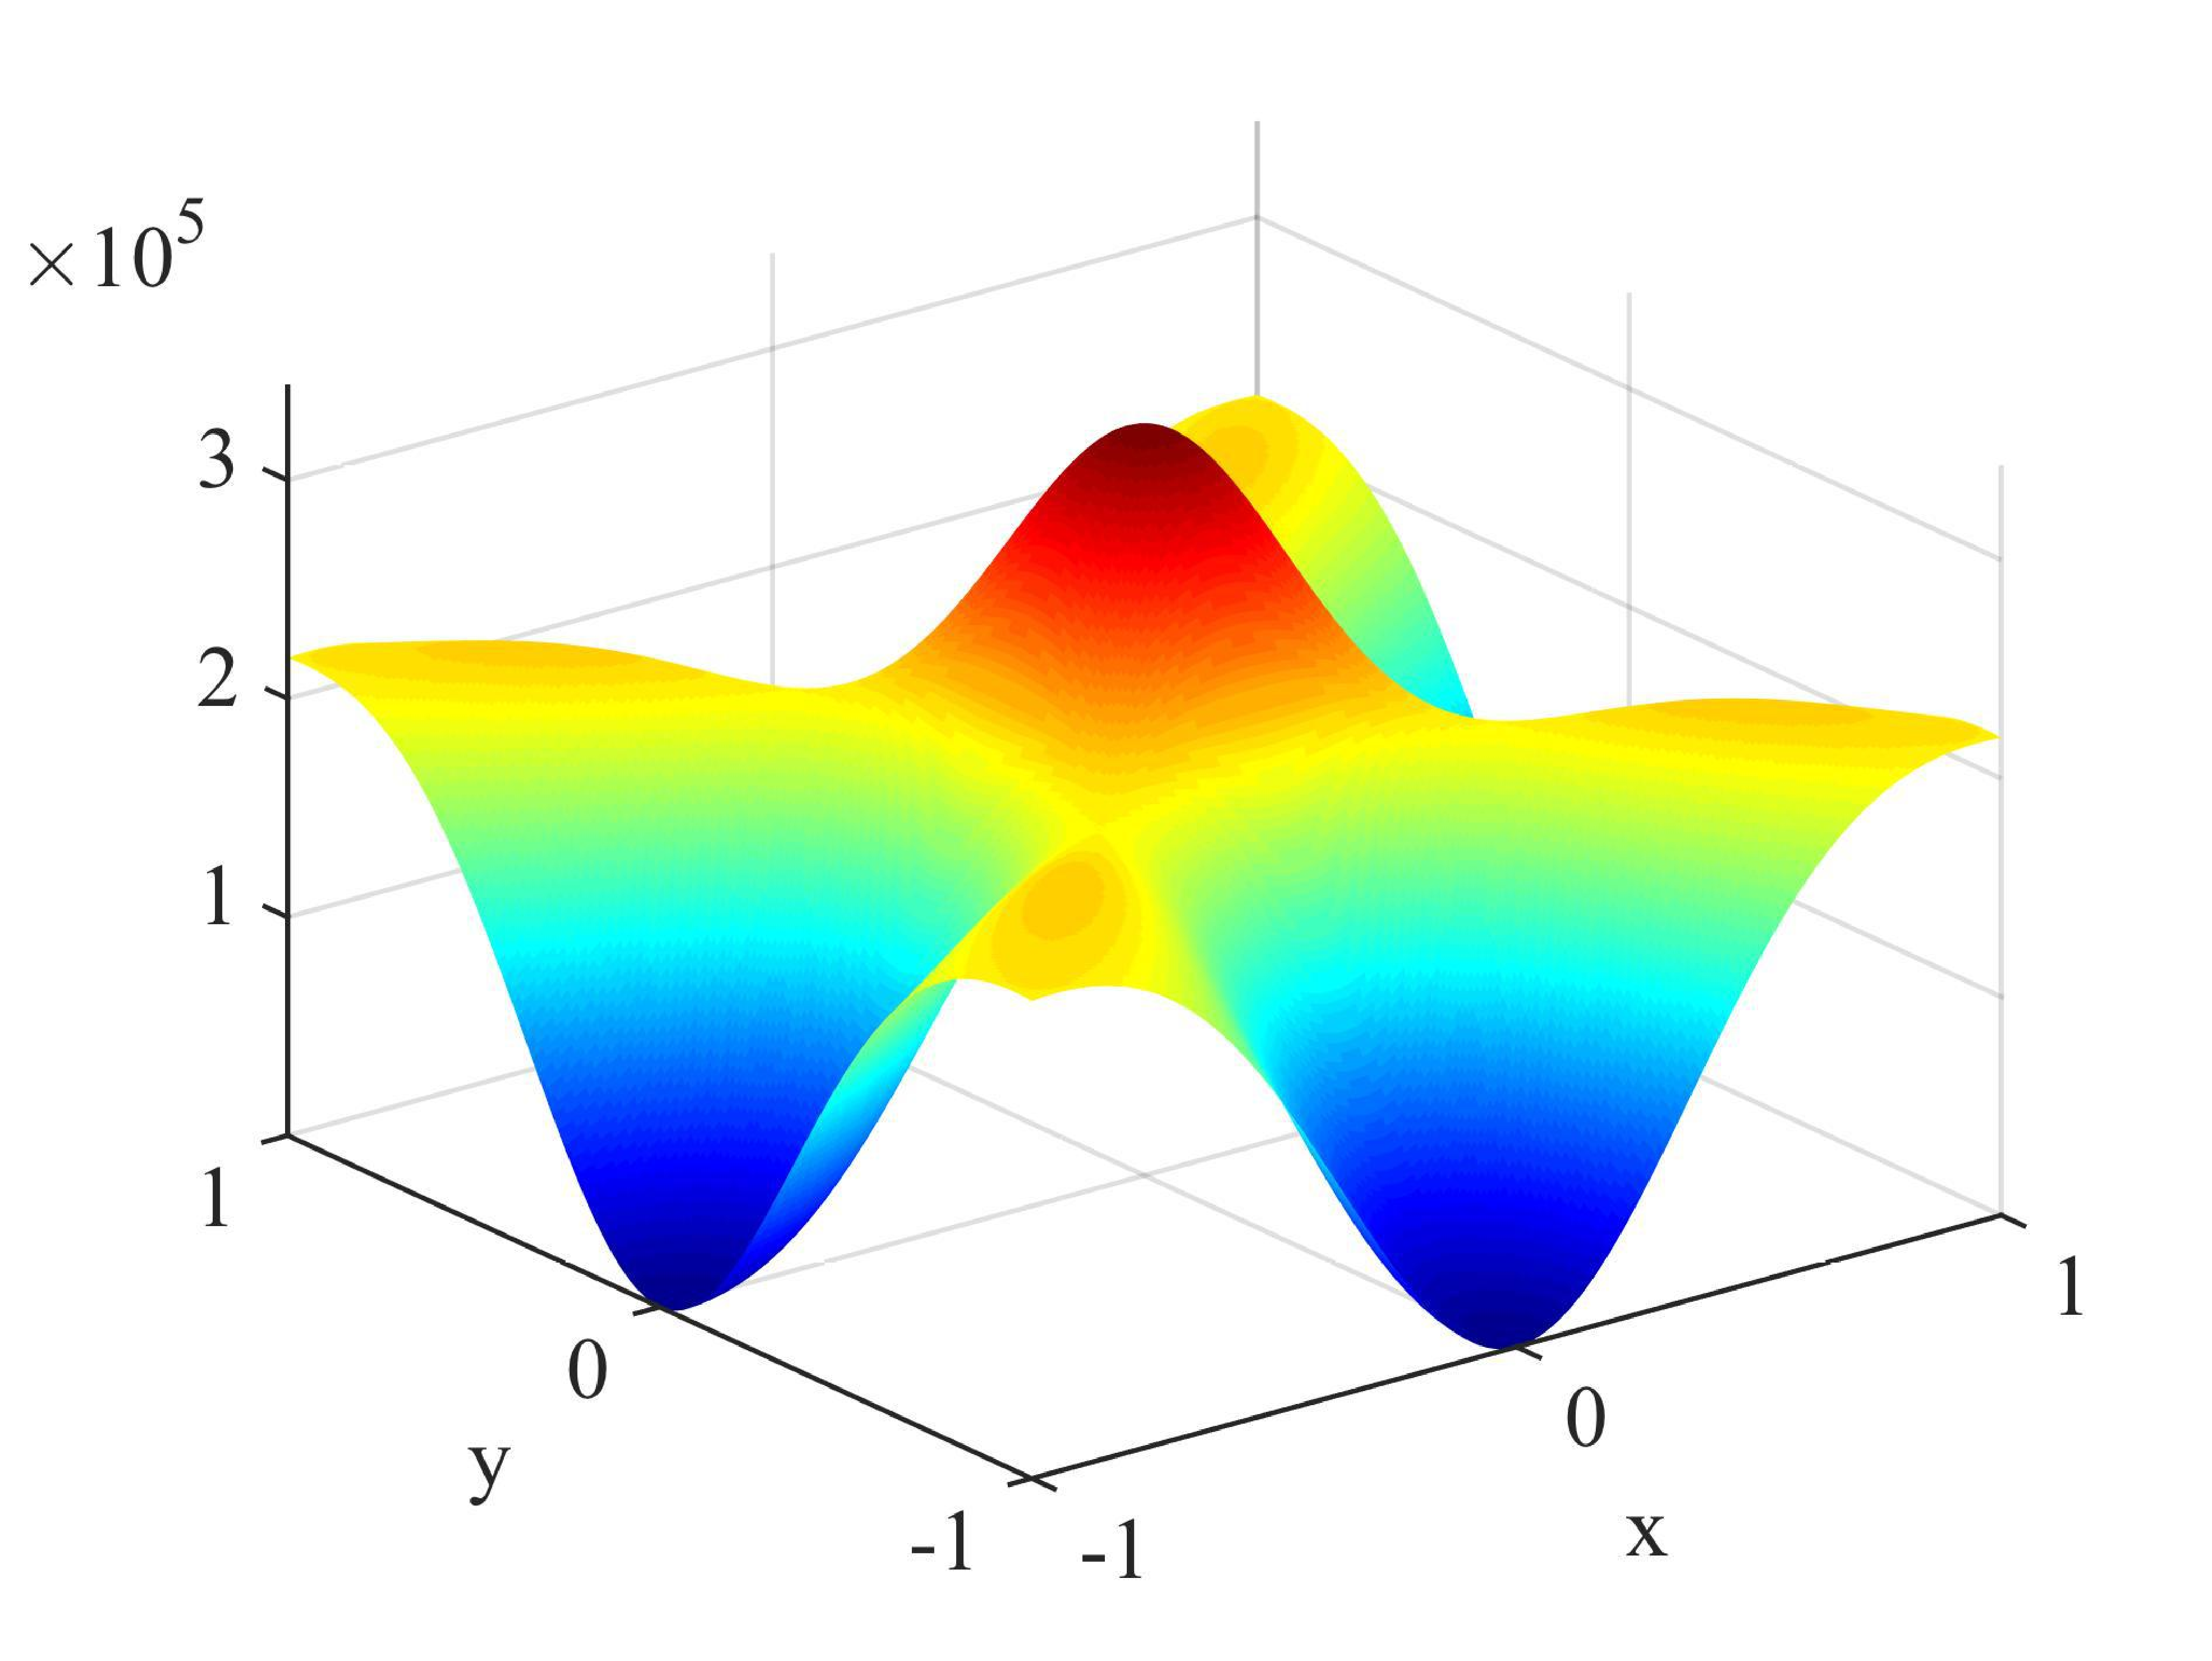
\includegraphics[width=0.45\textwidth]
   {figs/iso_shear_stereographic_detA.pdf}
 } \subfigure[Tangent]{
   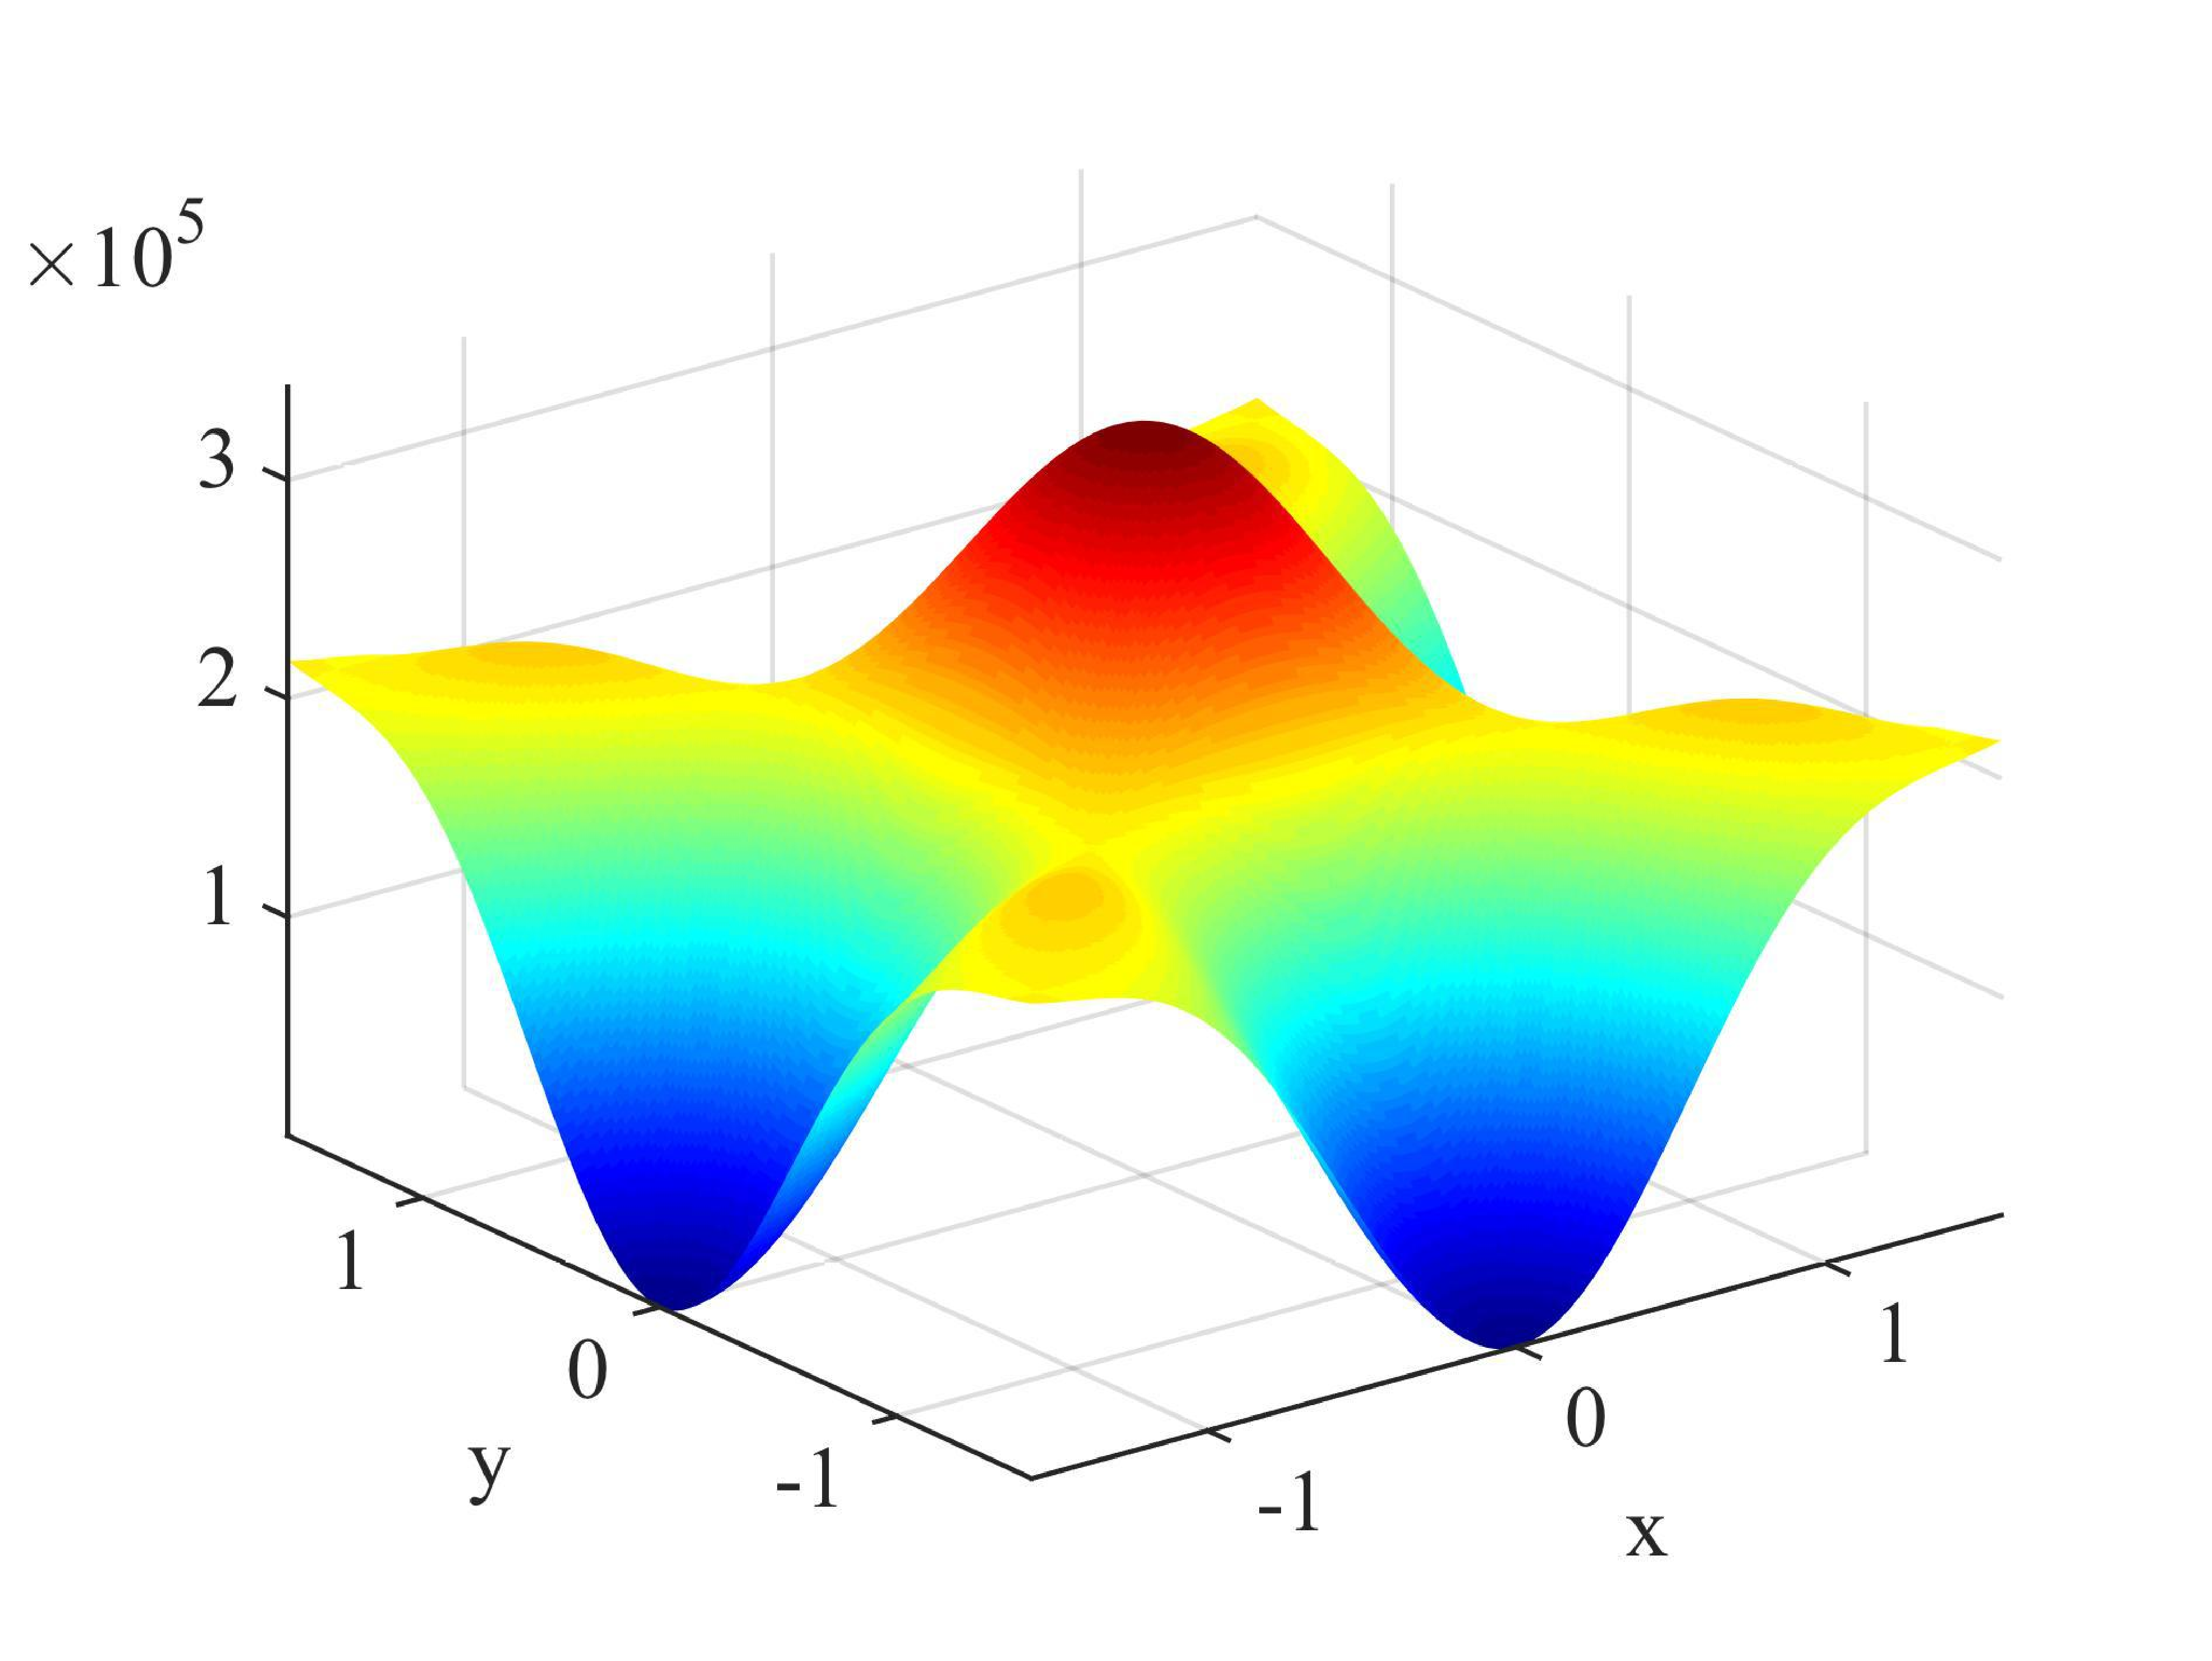
\includegraphics[width=0.45\textwidth]
   {figs/iso_shear_tangent_detA.pdf}
 }
   \caption{det$\bA$ landscapes at bifurcation
   for simple shear test on small deformation isotropic damage model.}
   \label{fig:iso_shear_detA}
 \end{figure}

\begin{figure}[H]
   \centering \subfigure[Spherical]{
   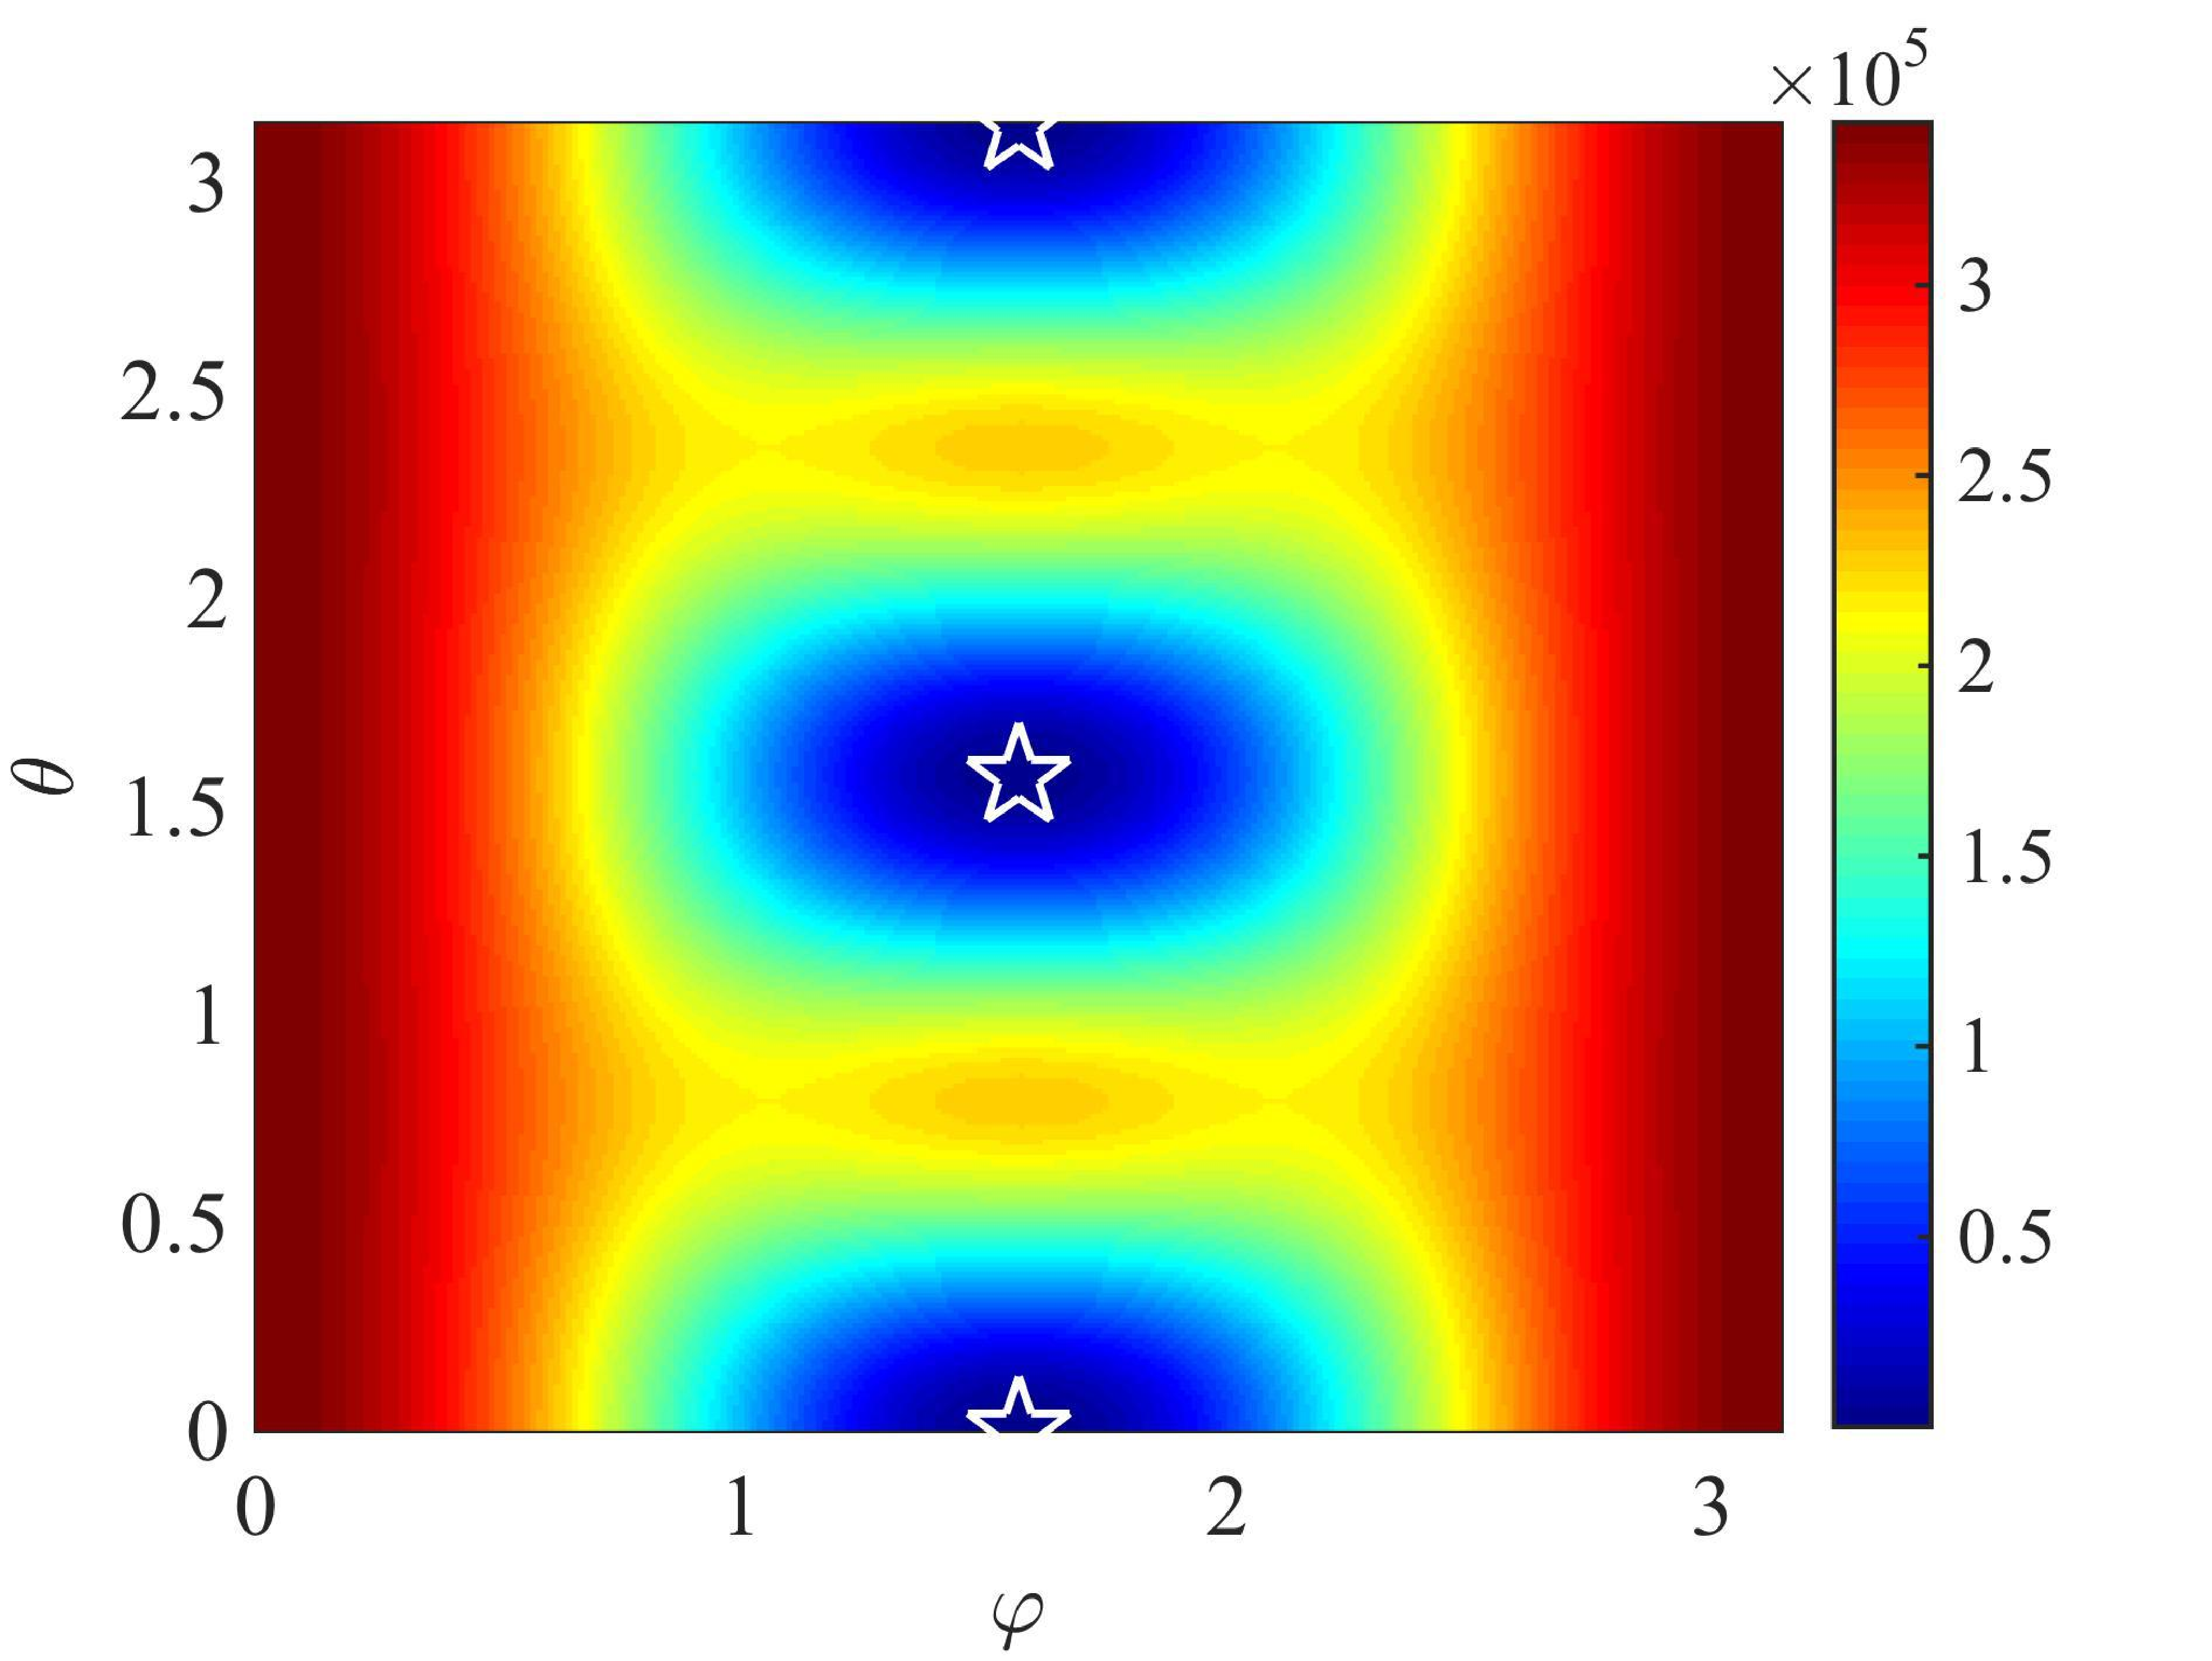
\includegraphics[width=0.45\textwidth]
   {figs/iso_shear_spherical_detAXplane.pdf}
 } \subfigure[Cartesian]{
   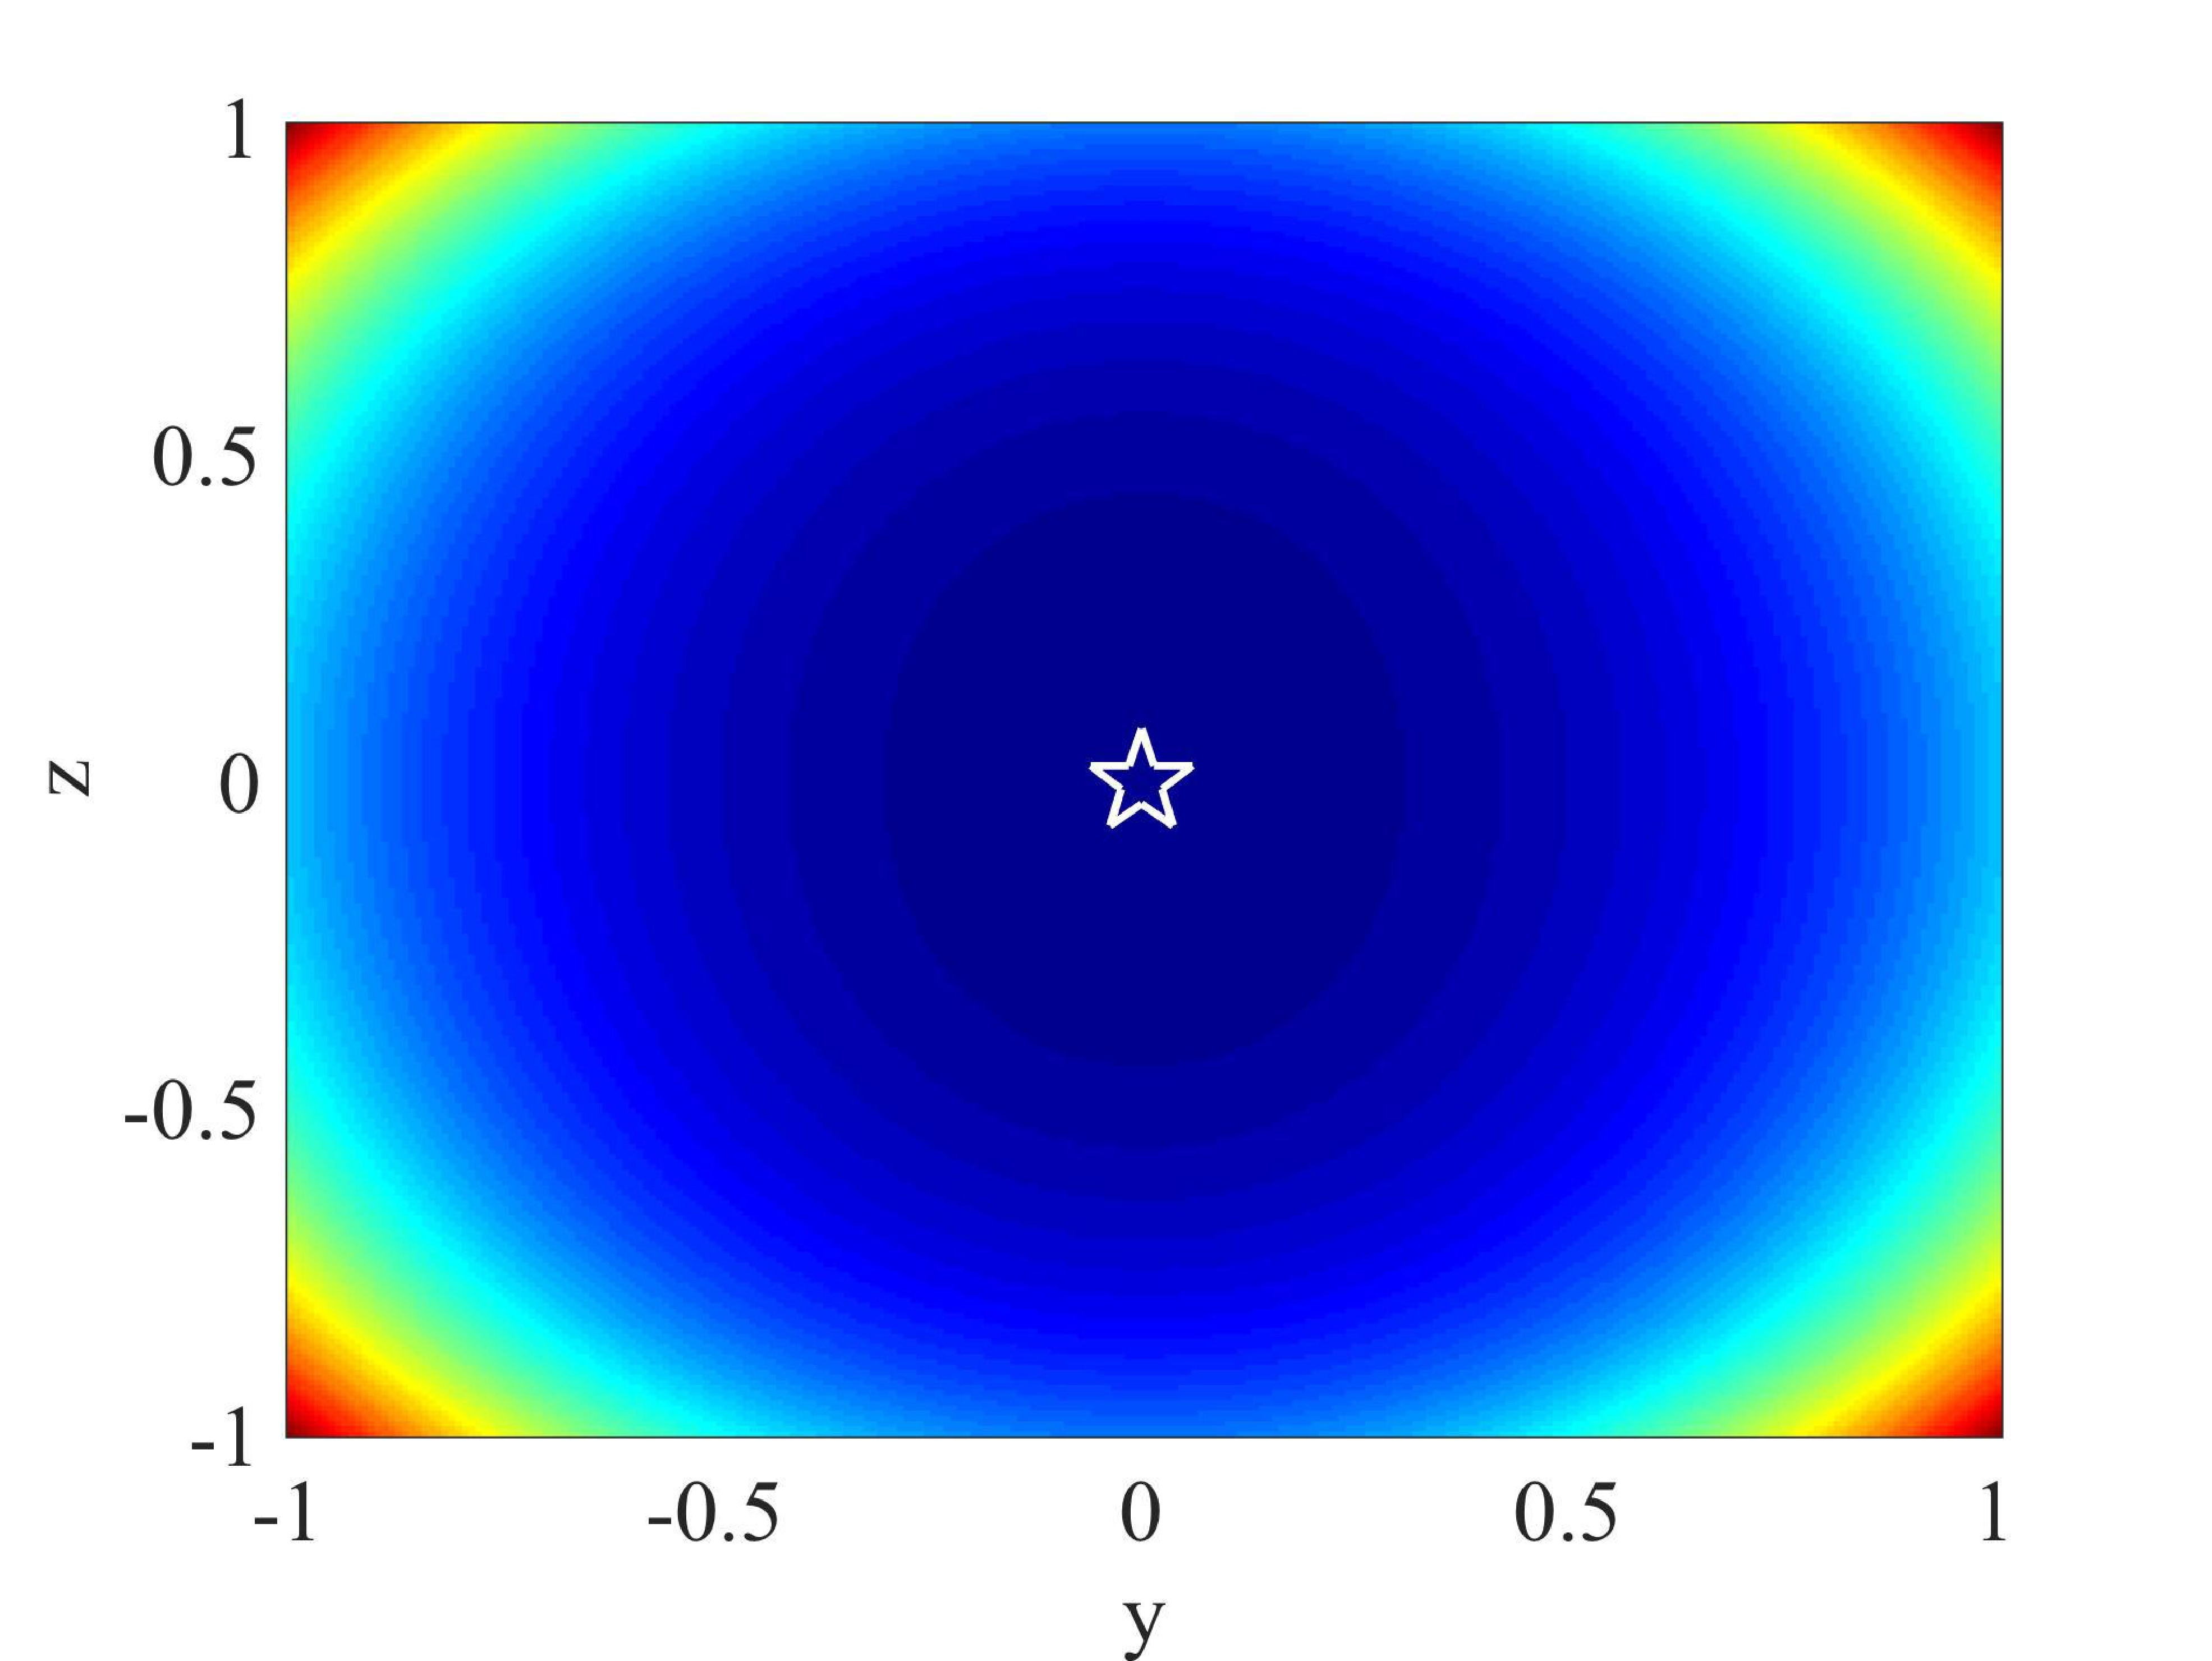
\includegraphics[width=0.45\textwidth]
   {figs/iso_shear_cartesian_detAXplane.pdf}
 } \subfigure[Stereographic]{
   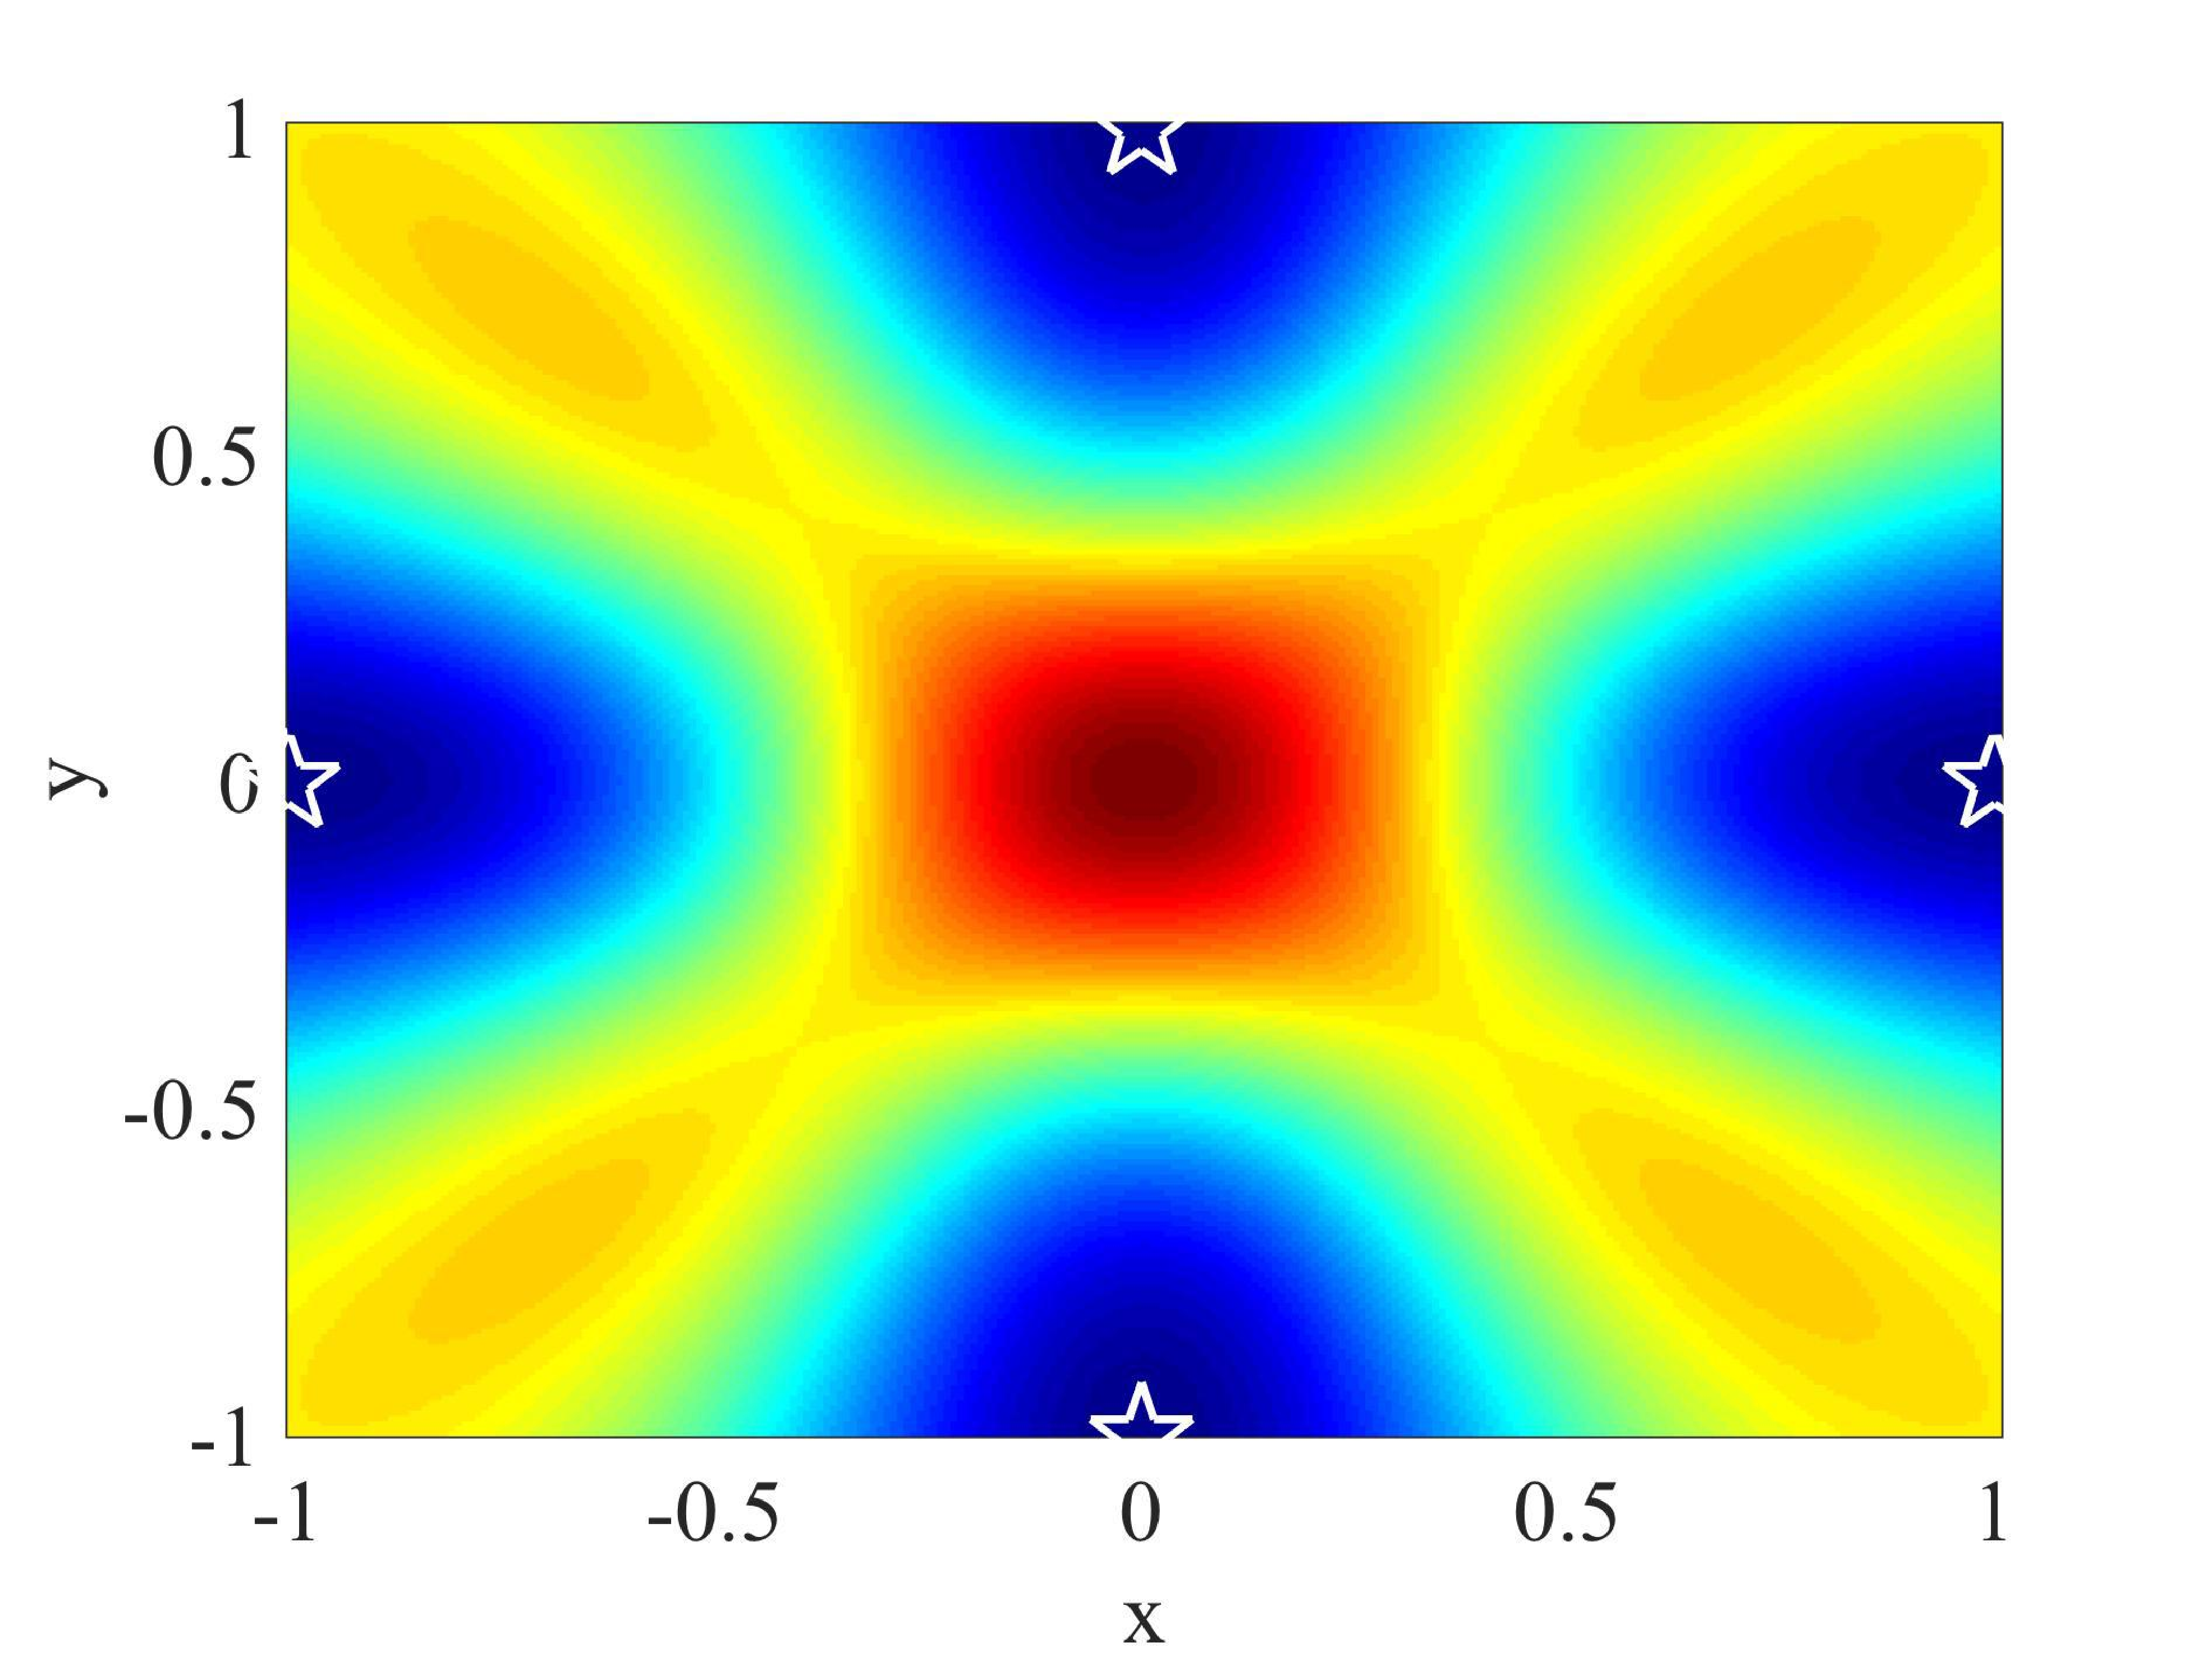
\includegraphics[width=0.45\textwidth]
   {figs/iso_shear_stereographic_detAXplane.pdf}
 } \subfigure[Tangent]{
   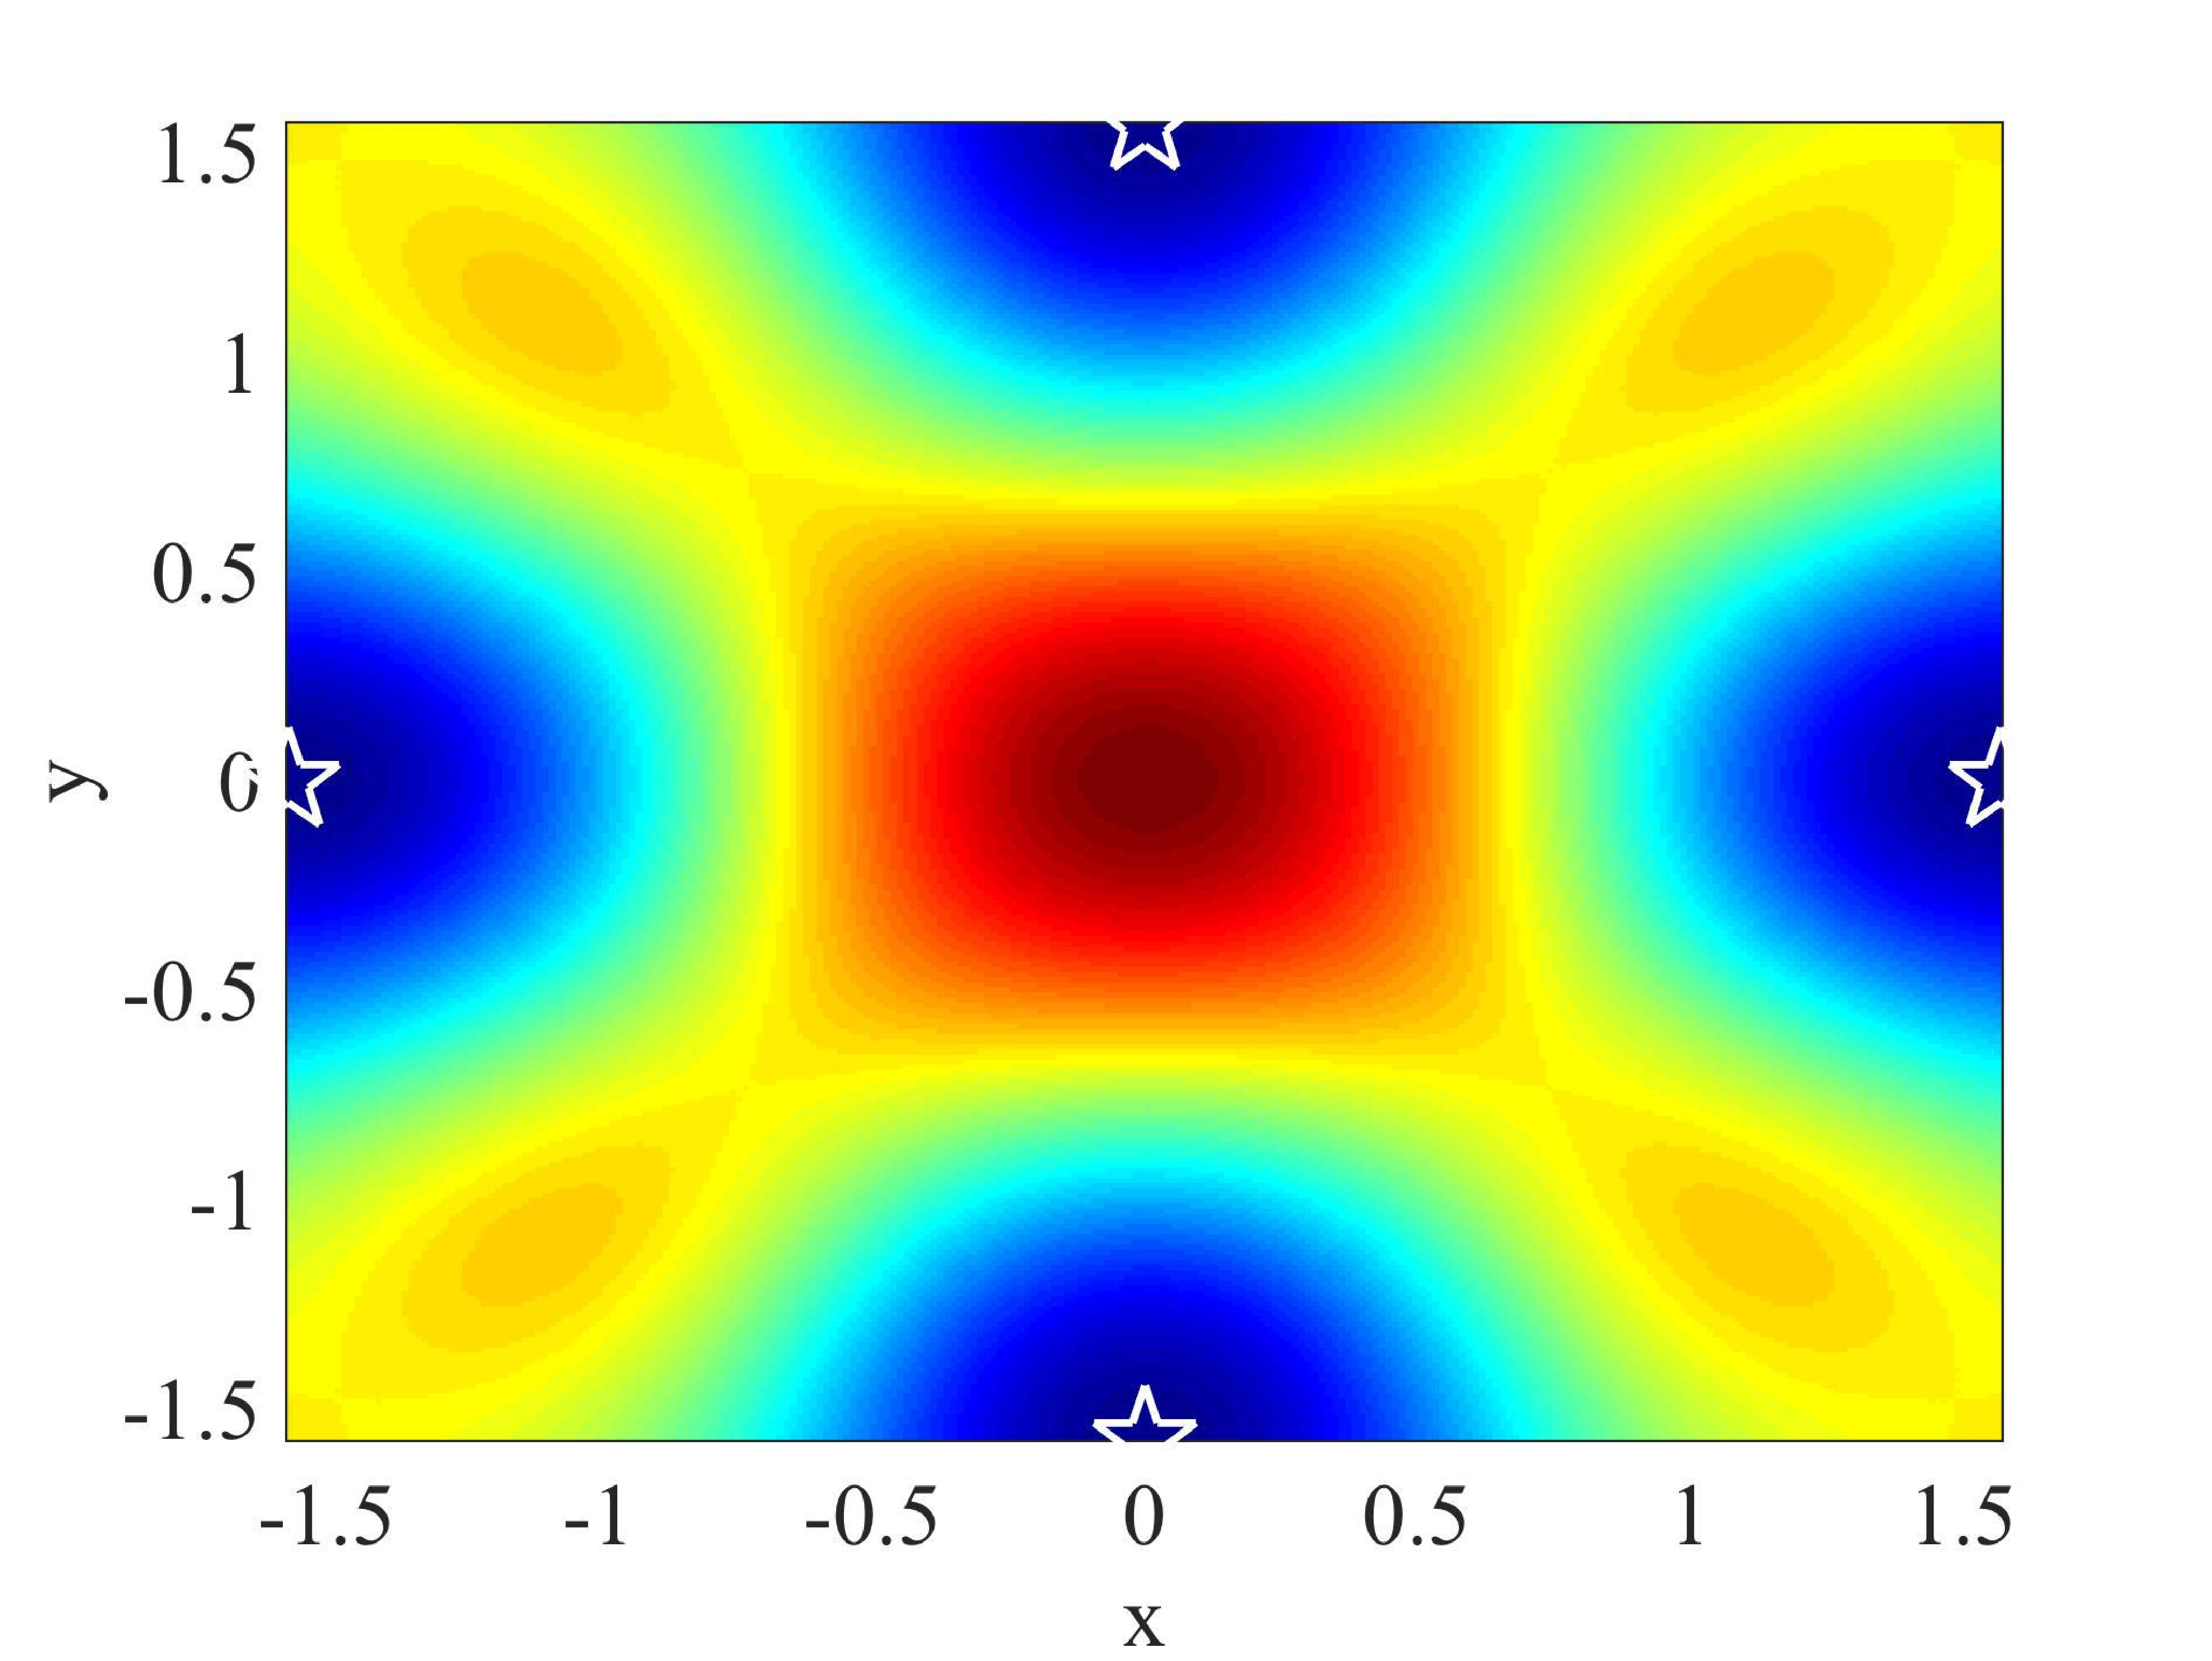
\includegraphics[width=0.45\textwidth]
   {figs/iso_shear_tangent_detAXplane.pdf}
 }
   \caption{Plane views det$\bA$ landscapes at bifurcation
   for simple shear test on small deformation isotropic damage model. 
   The white stars indicate global minimum point in the landscape.}
   \label{fig:iso_shear_detAXplane}
 \end{figure}

\subsection{Finite deformation anisotropic hyperelastic damage model}
\label{subsec:anisotropic}

The second material model tested is a finite deformation anisotropic 
hyperelastic damage model. By adding complexity to the material model, 
and hence the tangent modulus, we would like to study how is the 
performance of different parametrizations effected, especially in 
terms of the computational cost and robustness. As in the previous 
example, we first present the key feature of this proposed finite 
deformation material model.

\subsubsection{Model formulation}
The free energy function of the finite-deformation anisotropic 
hyperelastic damage model consists of an isotropic term and direction-
dependent terms. This type of energy formulation is motivated to 
capture behavior of materials with a isotropic matrix and some 
microfibers with preferred directions, such as the model proposed by
\cite{Chen.etal:2014} to capture behavior of hydrided nuclear cladding 
materials. We assume that the damage affects both the matrix and the 
microfibers. The free energy function is proposed to have the 
following form:

\begin{equation}\label{eq:aniso_energy}
  \Psi (\bC, \bM, \xi_m, \xi_i) 
    = (1-\xi_m) \Psi_m^0(\bC) 
    + \sum_{i}^{n} (1-\xi_i)\Psi_i^0(\bC, \bM)
\end{equation}

where $\bC$ is the Right Cauchy-Green tensor, $\bM$ is a
unit vector characterizing the preferred fiber direction. $\xi_m$ and
$\xi_i$ are the damage factors corresponding to the matrix and the 
$i$th fibers, respectively. In the following examples, we assume that 
there are two preferred fiber directions, i.e., $n=2$.

We adopt a compressible Neo-Hookean type energy function for the 
effective (undamaged) matrix component

\begin{equation}\label{eq:aniso_Psim0}
  \Psi_m^0 (\bC) 
    = \frac{1}{8}\lambda (\ln I_3)^2
    - \frac{1}{2}\mu \ln I_3 
    + \frac{1}{2}\mu( I_1 - 3)
\end{equation}

where $\lambda$ and $\mu$ are Lam\'{e}'s constant and shear modulus,
respectively.  

For microfibers, we adopt one particular form of strain-energy 
function (\cite{Holzapfel.etal:2010})

\begin{equation}
  \Psi_i^0(\bC, \bM) 
    = \frac{k_i}{q_i}
    \{ \exp[q_i(I_4 - 1)^2] \}
\end{equation}

where $k_i$ and $q_i$ are elastic constants for the $i$th fiber. 
The strain invariants $I_1$, $I_3$ and $I_4$ are defined as

\begin{equation}
  I_1 = \tr \bC, 
\end{equation}

\begin{equation}
  I_3 = \det \bC,
\end{equation}

\begin{equation}
  I_4 = \bM \cdot (\bC \bM)
\end{equation}

For damage evolution, the same evolution law as in \eref{eq:iso_xi} 
is used, except that for each phase of the material, i.e., each of the 
matrix and fibers, there will be a different set of parameters for
damage evolution (\cite{Chen.etal:2014}).

Given the energy function \eref{eq:aniso_energy}, the 4th order
tangent needed for bifurcation analysis can be derived by taking
derivative of the energy function with respect to some strain 
measures, in particular

\begin{equation}\label{eq:aniso_tangent}
  \tilde{\mathbb{C}} 
   = (1-\xi_m)\tilde{\mathbb{C}}_m^0 
   + \sum_i^n (1-\xi_i) \tilde{\mathbb{C}}_i^0
   -\beta_m \xi_m' (\bS_m^0 \otimes \bS_m^0 )
   - \sum_i^n \beta_i \xi_i' (\bS_i^0 \otimes \bS_i^0 )
\end{equation}

where $\beta_m\neq 0$ if and only if damages evolves in matrix, and
$\beta_i \neq 0$ if and only if damages evolves in fiber $i$. The 
effective tangent modulus tensor is given by

\begin{equation}\label{eq:aniso_tangent1}
  \tilde{\mathbb{C}}_m^0 = 
    4\frac{\partial ^2 \Psi_m^0}{\partial\bC \partial\bC}
\end{equation}

\begin{equation}\label{eq:aniso_tangent2}
  \tilde{\mathbb{C}}_i^0 =  
    4 \frac{\partial ^2 \Psi_i^0}{\partial\bC \partial\bC}
\end{equation}

It should be noted that the 4th-order tangent $\tilde{\mathbb{C}}$ 
from \eref{eq:aniso_tangent} is computed as the derivative of strain 
energy with respect to the right Cauchy-Green tensor. The strong 
ellipticity condition \eref{eq:strong-ellipticity} requires the 
tangent $\mathbb{C}$ to be computed as a derivative with respect to 
the deformation gradient. These two tangents can be converted using 
the following relation (in indicial notation)

\begin{equation}
  \mathbb{C}_{ijkl} = S_{lj}\delta_{ik}
    + F_{ip} \tilde{\mathbb{C}}_{pjlq} F_{kq}
\end{equation}

where $\bS$ is the 2nd Piola-Kirchhoff tensor, $\bdelta$ is the 
Kronecker delta and $\bF$ is the deformation gradient.

\subsubsection{Uniaxial tension test}

The finite deformation anisotropic model is tested under monotonically
increased uniaxial tension test. The material properties for both 
matrix and fibers are listed in Table \ref{tab:aniso_material}.

\begin{table}[H]
  \begin{center}
    \begin{tabular}{ l l l l }
      \toprule
      \it{Matrix}:
      &
      
      &
     
      \it{Fibers}:
      
      &
      \\
      Lam\'{e}'s constant
      &
      $\lambda=80$
      &
      Elasticity constants
      &
      $k_1 = k_2 = 100$
      \\
      Shear modulus
      &
      $\mu = 80$
      &
      Elasticity constants
      &
      $q_1 = q_2 = 1.0$      
      \\
      Damage variable  
      &
      $\xi_{\infty(m)} = 1.0$
      &
      Damage variable
      &
      $\xi_{\infty(1)} = \xi_{\infty(2)} = 1.0$      
      \\
      Damage variable   
      &
      $\tau_m = 4.0$
      &
      Damage variable
      &
      $\tau_1 = \tau_2 = 4.0$
      \\
      &
      
      &
      Direction vector
      &
      $\bM_1 = \{ 0.8,~0.6,~0.0\}$
      \\
      &

      &
	       
      &
      $\bM_2 = \{ 0.8,-0.6,~0.0\}$
      \\
      \bottomrule
    \end{tabular}
    \caption{Material properties for anisotropic damage model}
    \label{tab:aniso_material}
  \end{center}
\end{table}

The axial stress vs. stretch behavior in the uniaxial tension test is 
shown in Figure \ref{fig:aniso_stress_stretch}(a). The material 
bifurcation is marked on the stress vs. stretch plot. As detailed in 
Section \ref{sec:detection}, a two-step procedure is adopted: an 
initial sampling followed by a Newton-type iterative solve. With the 
adaptive time step algorithm, the precise time (upto the set 
tolerance) of bifurcation can be detected. In this loading test, all 
five parametrizations detect bifurcation at the same time, i.e., when 
the axial component of the deformation gradient $F_11 = 1.1954$. The 
degradations of the determinant function ${\rm det}\bA$ for all five 
parametrizations are shown in Figure \ref{fig:aniso_stress_stretch}(b)

\begin{figure}[H]
  \centering \subfigure[]{
    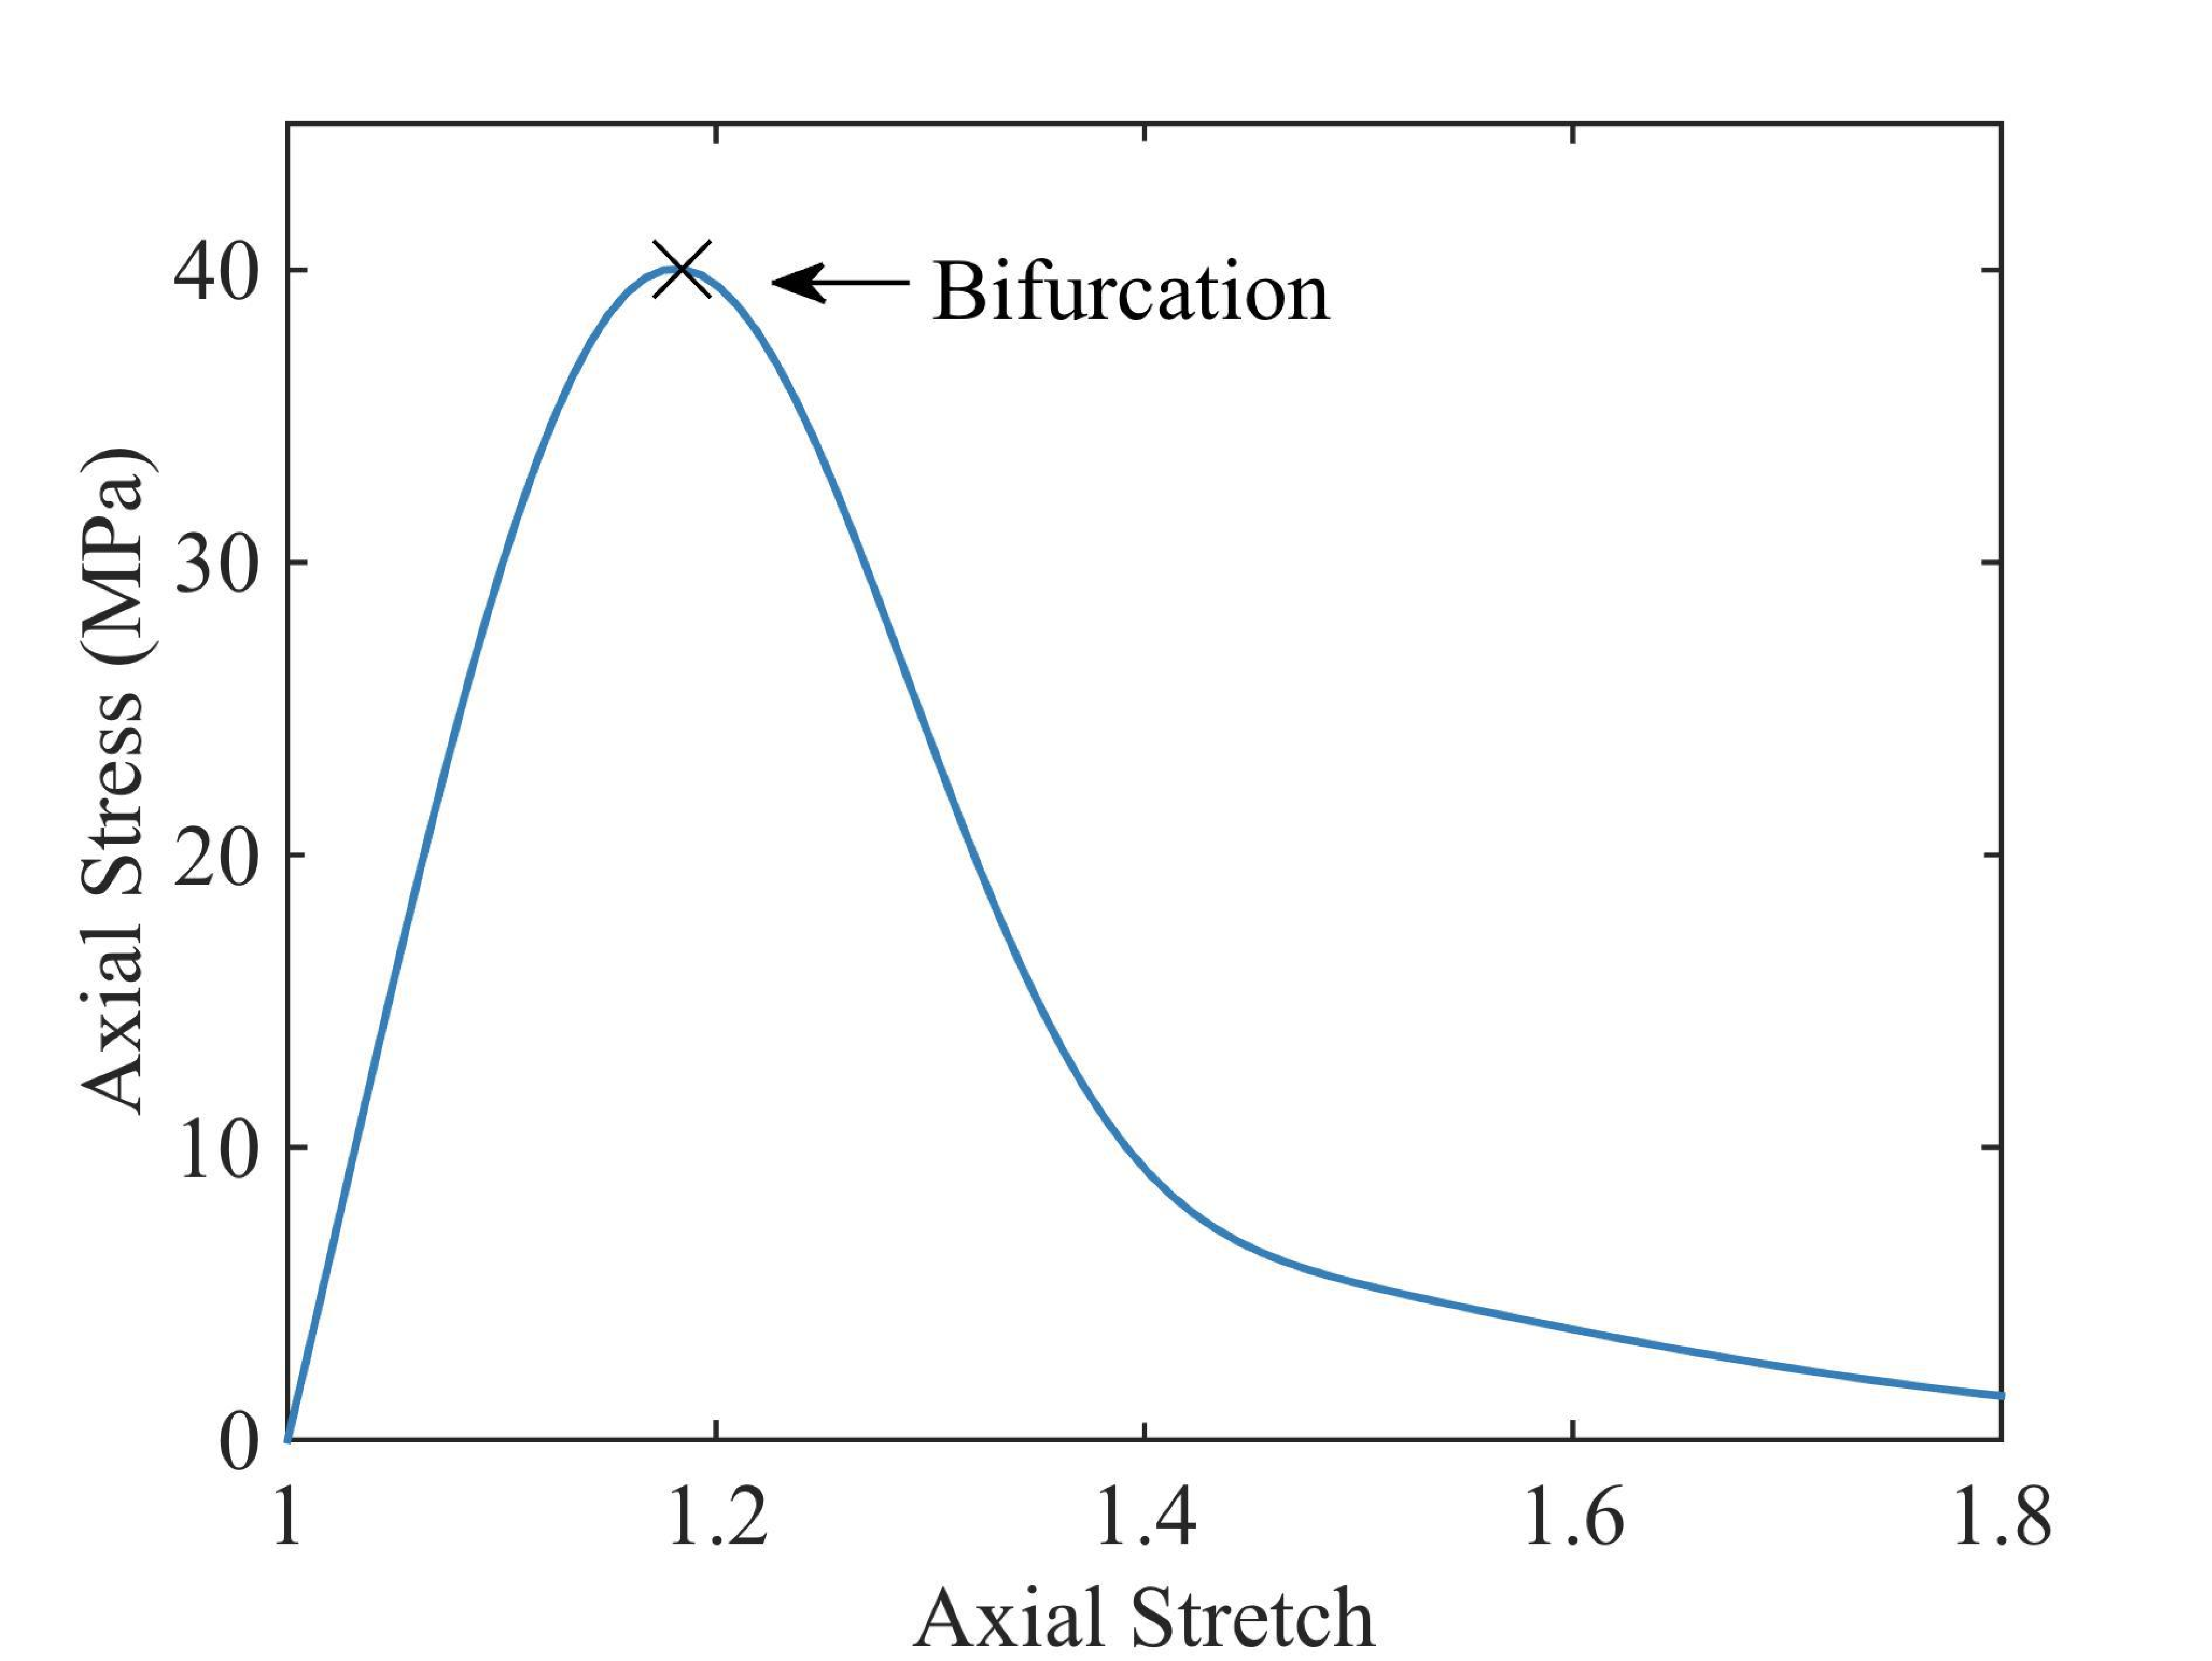
\includegraphics[width=0.45\textwidth]
    {figs/aniso_uniaxial_stress_stretch.pdf}
  } \subfigure[]{
    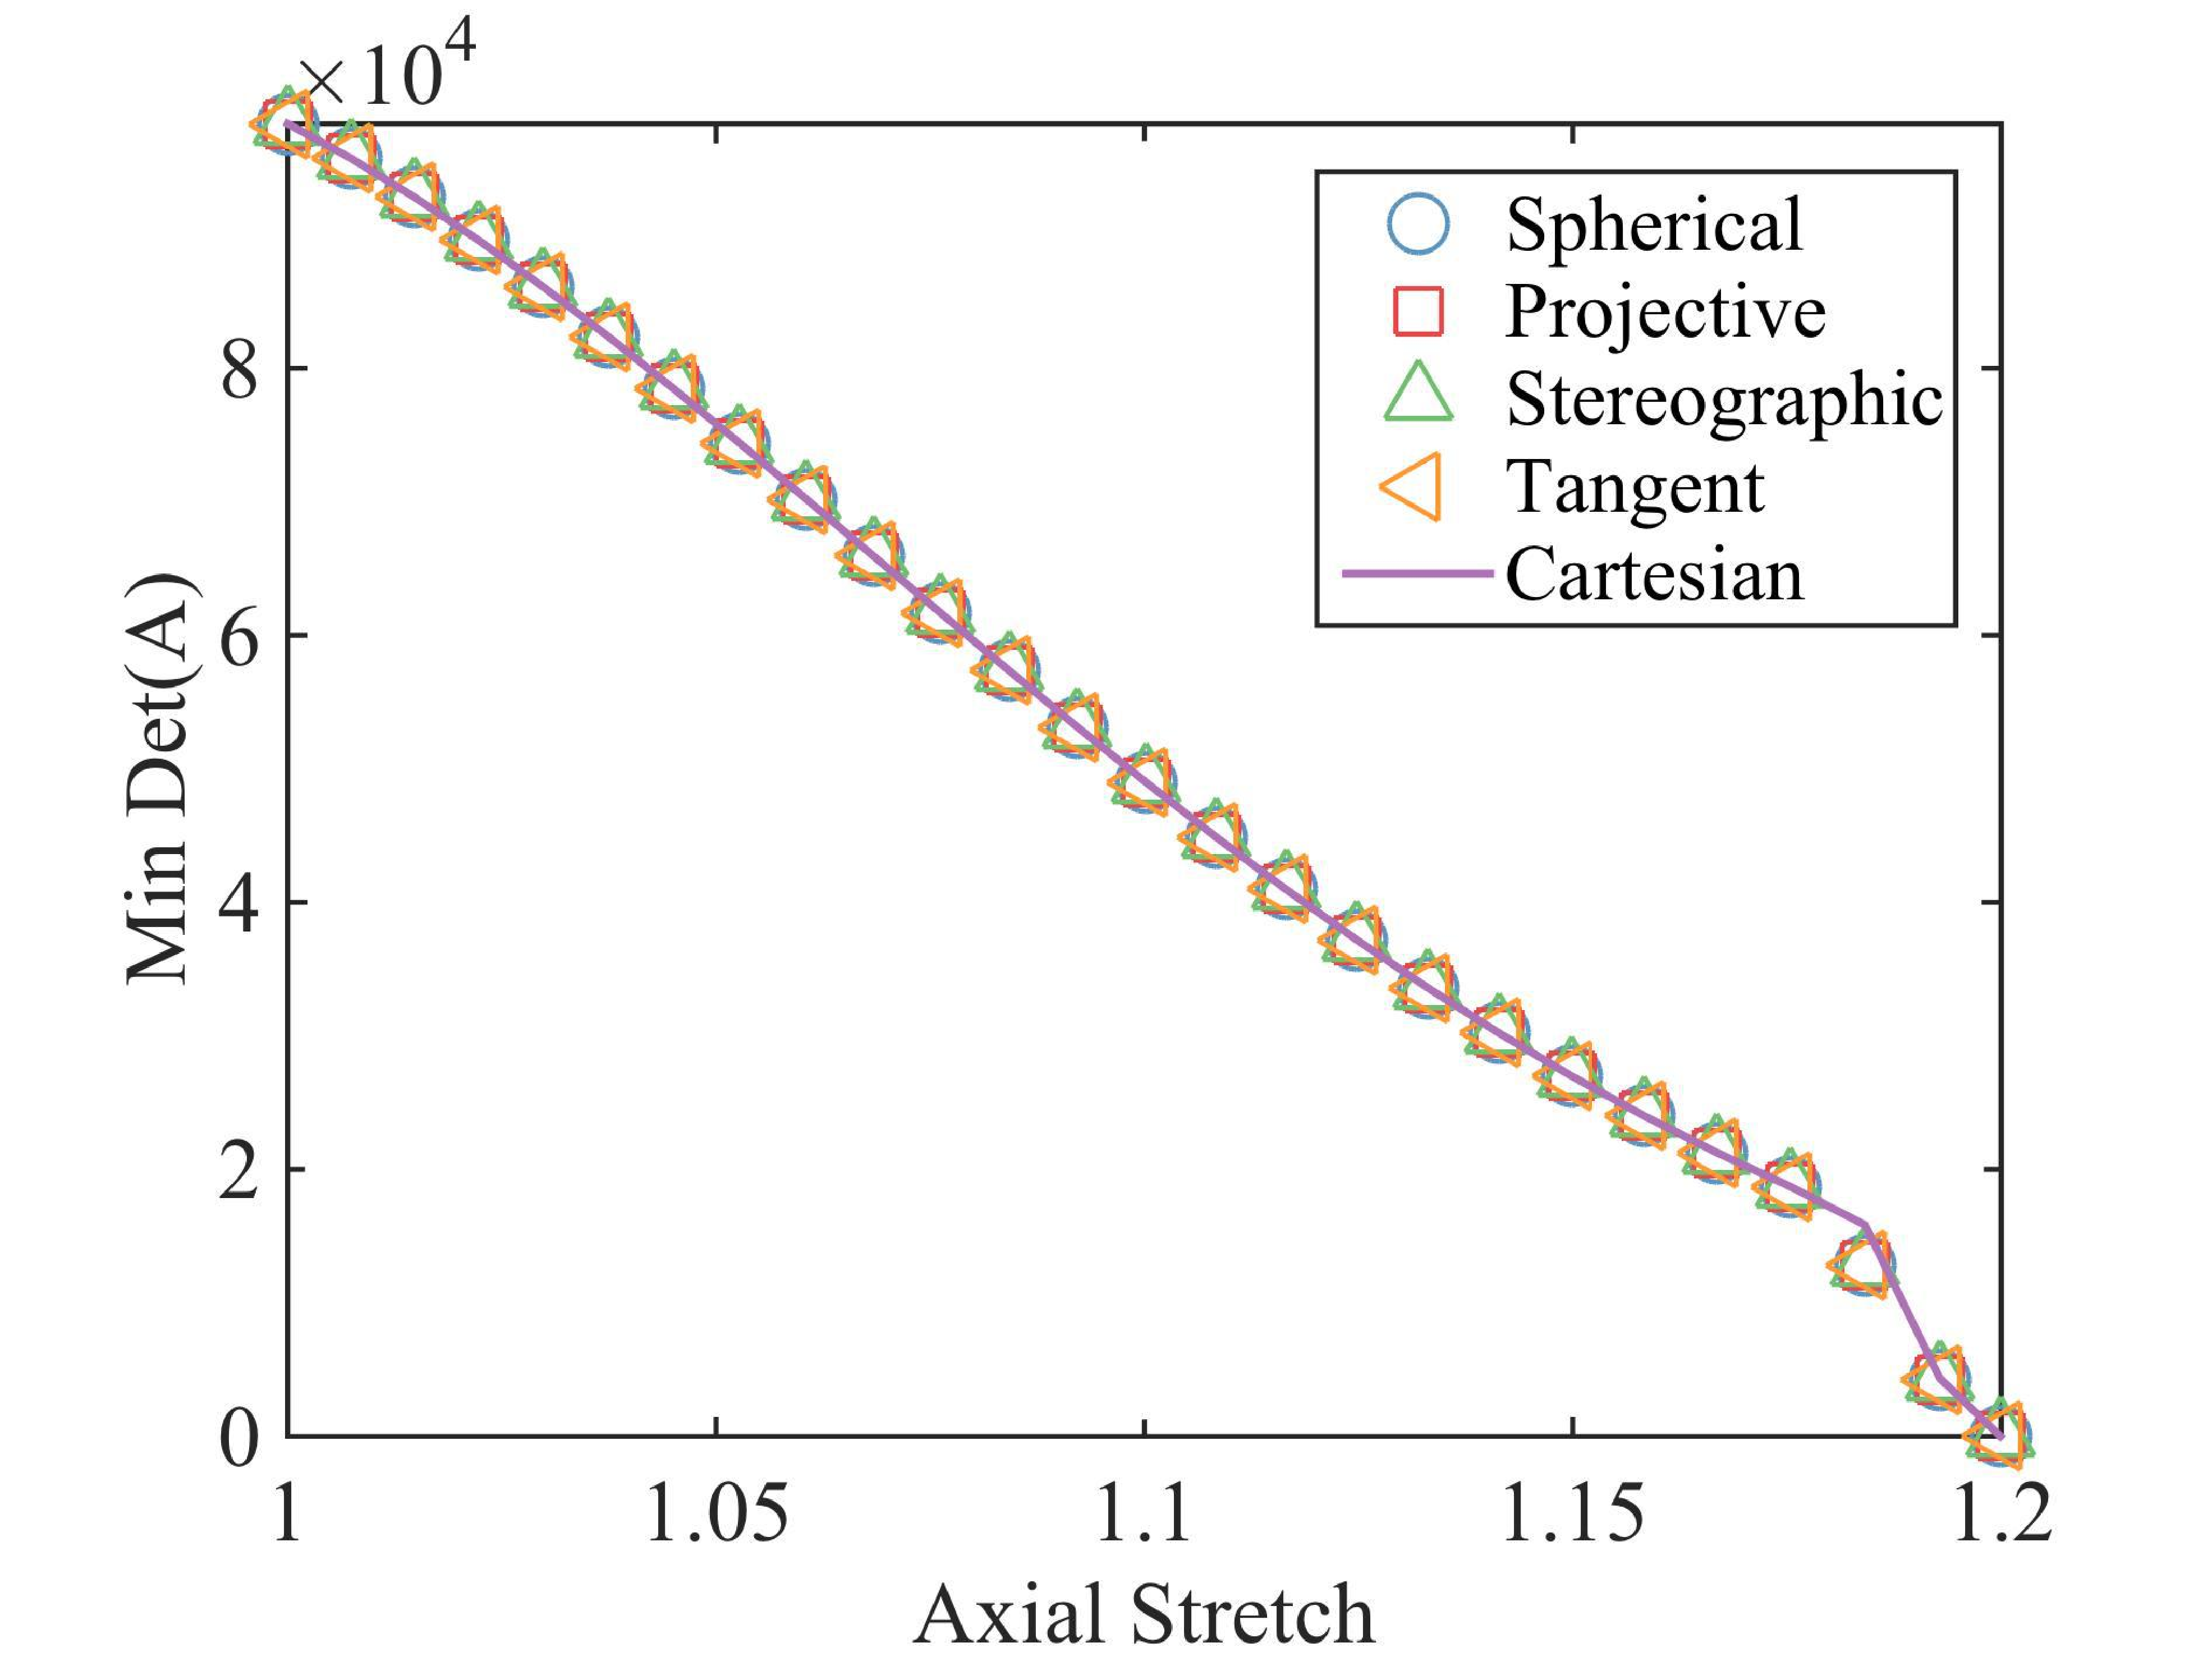
\includegraphics[width=0.45\textwidth]
    {figs/aniso_uniaxial_mindetA_stretch.pdf}
  }
  \caption{Uniaxial tension test on finite deformation 
  anisotropic damage model: 
  (a)stress strain behavior, with red cross indicating bifurcation, and
  (b) degradation of det$\bA$ for different
  parametrizations.}
  \label{fig:aniso_stress_stretch}
\end{figure}

As in the previous example, the computational cost of different 
parametrizations at the loading increment leading to bifurcation is 
recorded and shown in Table \ref{tab:aniso_uniaxial_runtime}. Again, 
the density of the initial sampling is represented by the sampling 
interval and the number of sampling points. In general, as the number 
of sampling points decreases, so does the computational cost. However, 
the fewer sampling points also leads to a very poor initial guess for 
the Newton iterative solve, which may cost more time to arrive at a 
converged solution if there is one at all. Because of the added 
complexity of the material model, different parametrizations are more 
sensitive to the density of the initial sampling grids. The spherical 
parametrization is unable to detect correctly the bifurcation when the 
sampling interval is greater than 0.4. The stereographic, projective 
and tangent parametrizations, though more robust in this case, are 
computationally more expensive. The cartesian parametrization is 
computationally efficient and at the same time, relatively insensitive 
to the sampling interval. 

\begin{table}[H]
  \begin{center}
    %\begin{tabular}{ p{1.5cm} | p{1.7cm} p{1.7cm} p{1.7cm} p{1.7cm} p{1.7cm} }
    \begin{tabular}{c c | r r r r r}
      \toprule
      Sampling   & Sampling &   \multicolumn{5}{c}{Run time ($\mu$s)}	\\   
      interval     & points     &  Spherical    &   Stereographic  &   Projective  &   Tangent   & Cartesian  \\
      \midrule         
      0.05      &      41     &      508     &    351        &       5671       &       368        &      476           \\
      0.1        &      21     &      291      &    260        &       993         &       275 &      230           \\
      0.2        &      11     &      n/a      &    225        &       367          &       n/a         &      224            \\
      0.3        &      7       &      221      &    220         &       327         &       n/a         &      340           \\
      0.4        &      5       &      283      &    n/a        &       245          &       297        &      205           \\       
      0.5        &      5       &	  n/a      &    402         &       252          &      405         &      146           \\
      0.6        &      3       &	  n/a      &    220         &       n/a         &       360        &      183           \\
      0.7        &      3       &	  n/a     &    395 	      &        n/a         &       205         &      n/a            \\
      0.8        &      3       &      n/a      &    n/a        &        n/a         &       303        &       n/a            \\	      
      0.9        &      3       &	  n/a      &    n/a         &        n/a         &       n/a        &       n/a         \\	
      1.0        &      3       &      n/a      &    n/a	      &       n/a          &       n/a        &       n/a          \\	
      1.5        &      1       &	  n/a      &    n/a	      &       n/a          &       n/a        &       n/a          \\	       
      \bottomrule
    \end{tabular}
    \caption{Computational cost of different parametrizations in 
    uniaxial tension test at loading increment leading to bifurcation. 
    `n/a' means the parametrization fails to detect bifurcation in 
    this loading increment.}
    \label{tab:aniso_uniaxial_runtime}
  \end{center}
\end{table}


To gain insights into the influence of parametrizations on the 
determinant function det$\bA$ as loading proceeds, we plot the 
landscapes at four different axial stretch levels for different 
parametrizations, as shown in Figures \ref{fig:aniso_spherical_detA} - 
\ref{fig:aniso_cartesian_detA}.

\begin{figure}[H]
   \centering \subfigure[$F_{11}=1.0074$]{
   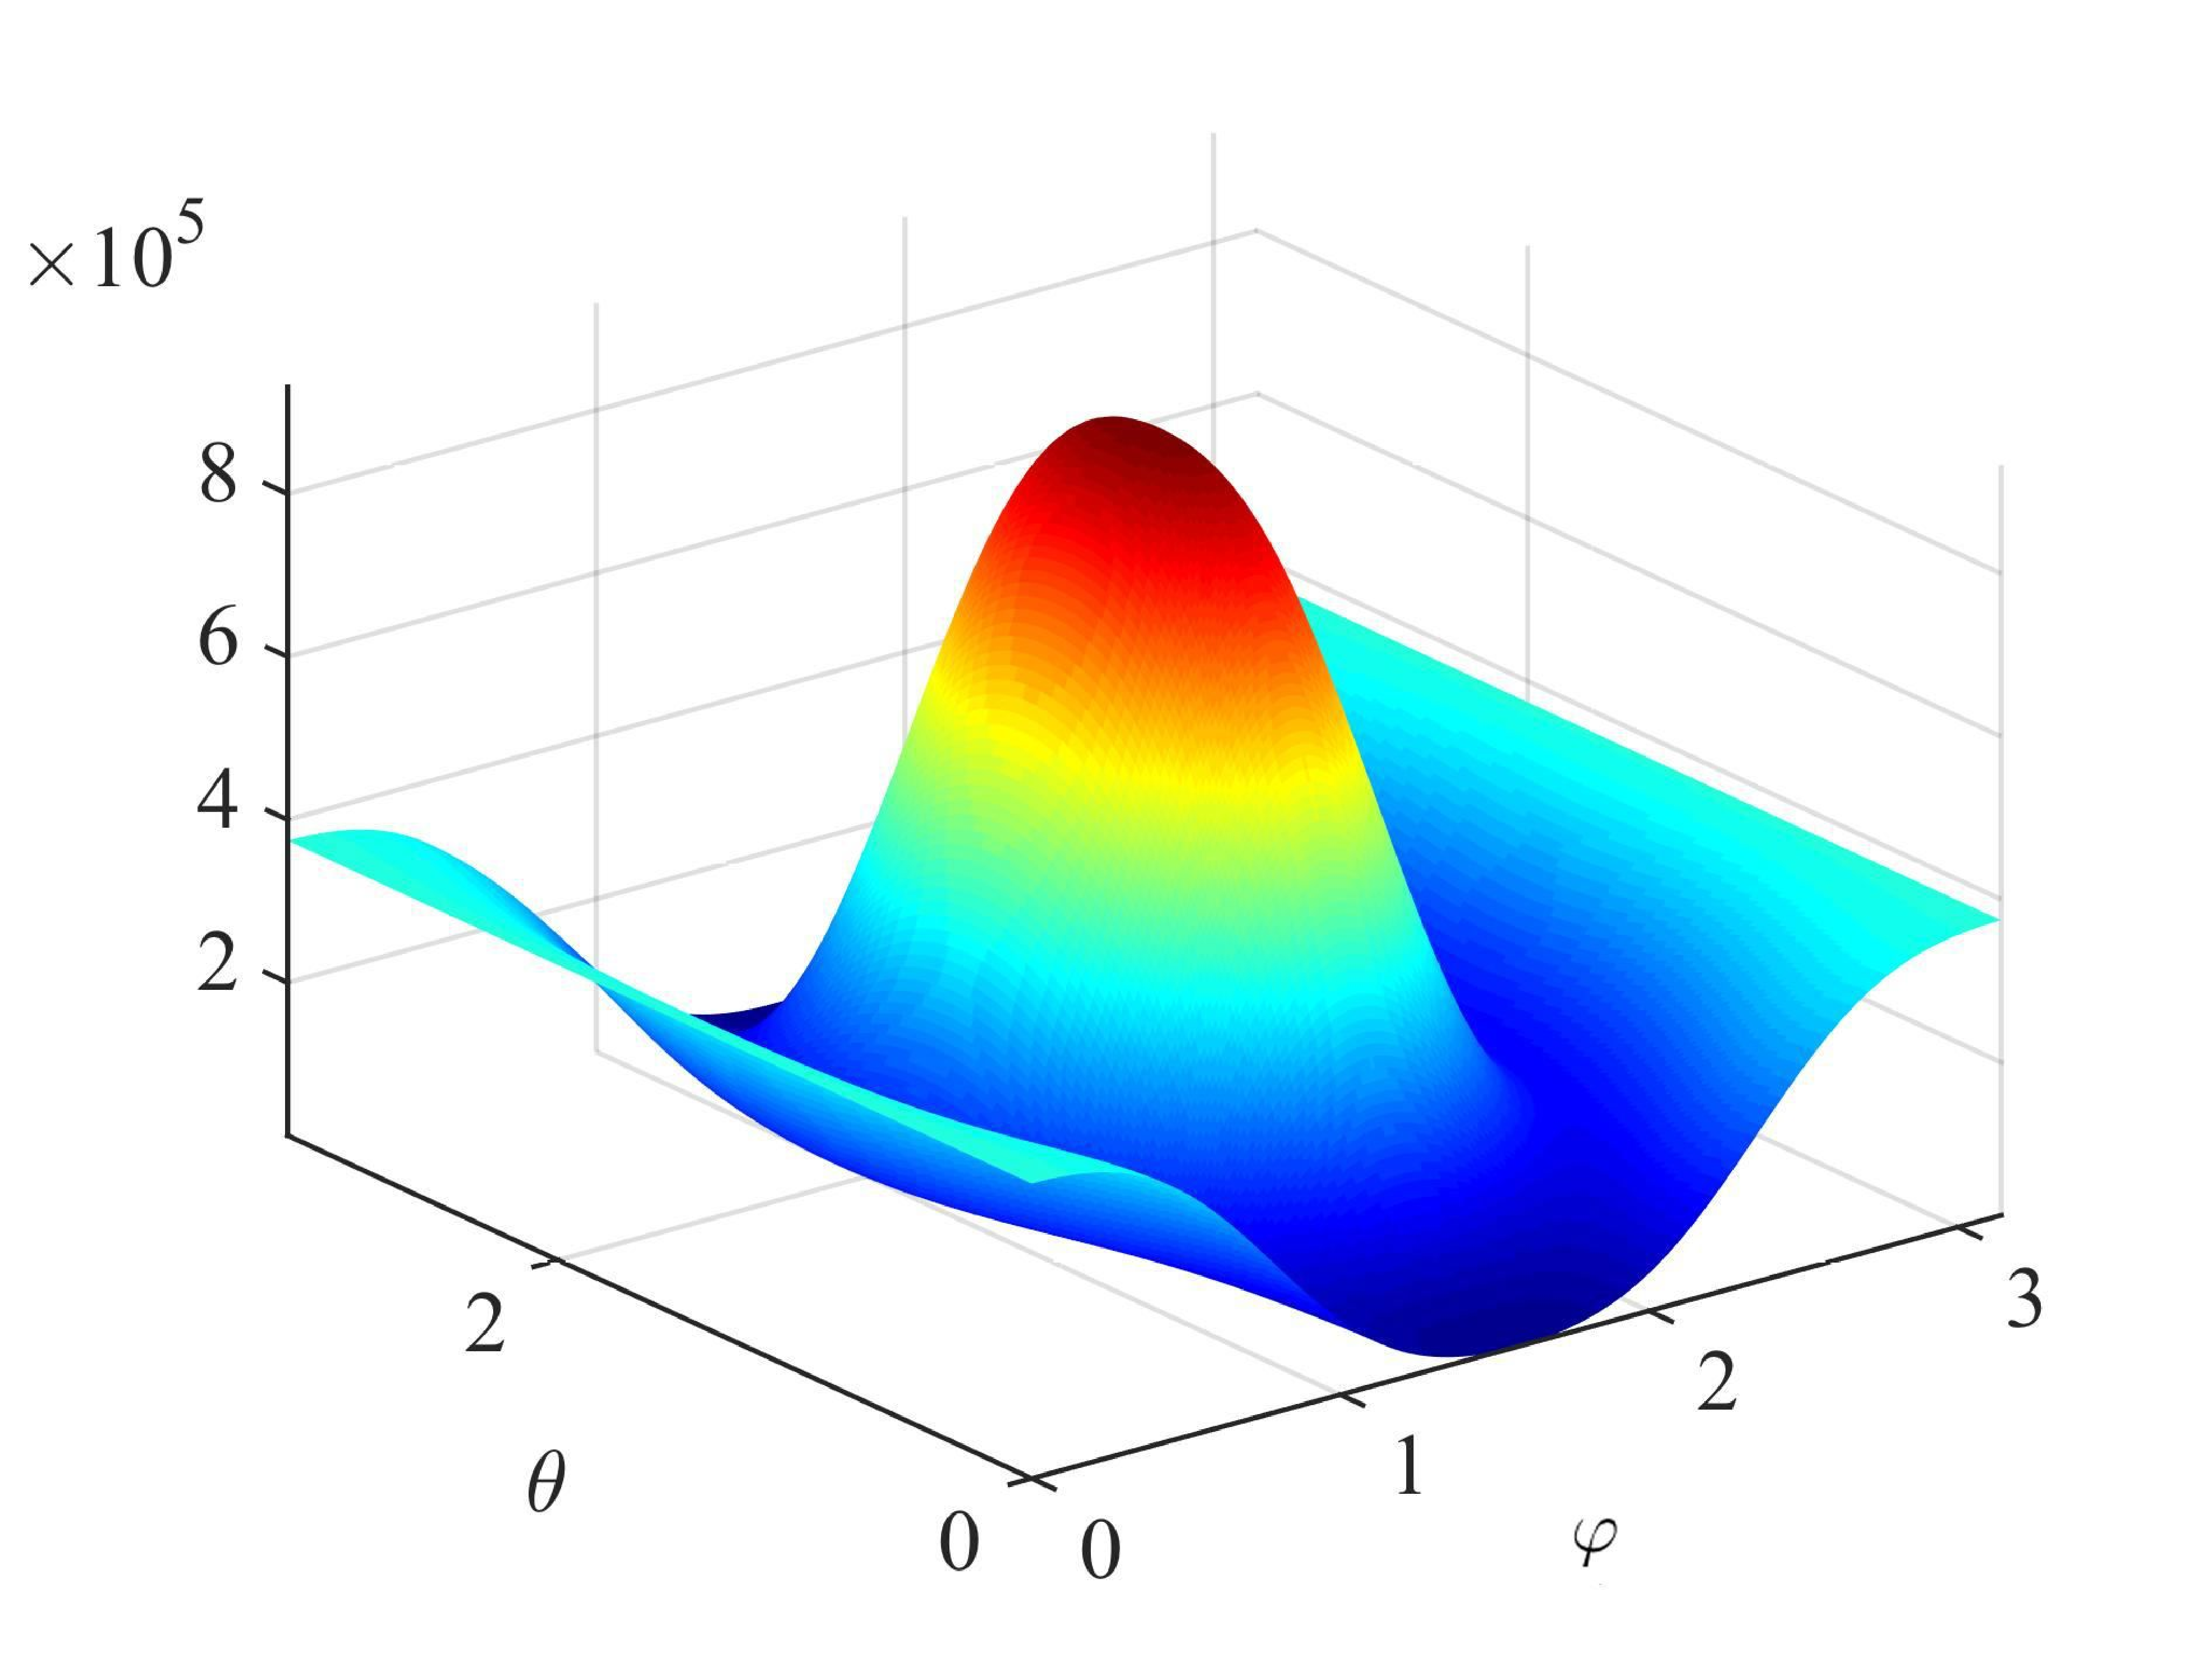
\includegraphics[width=0.45\textwidth]
   {figs/aniso_uniaxial_spherical_detA_F1p0074.pdf}
 } \subfigure[$F_{11}=1.0762$]{
   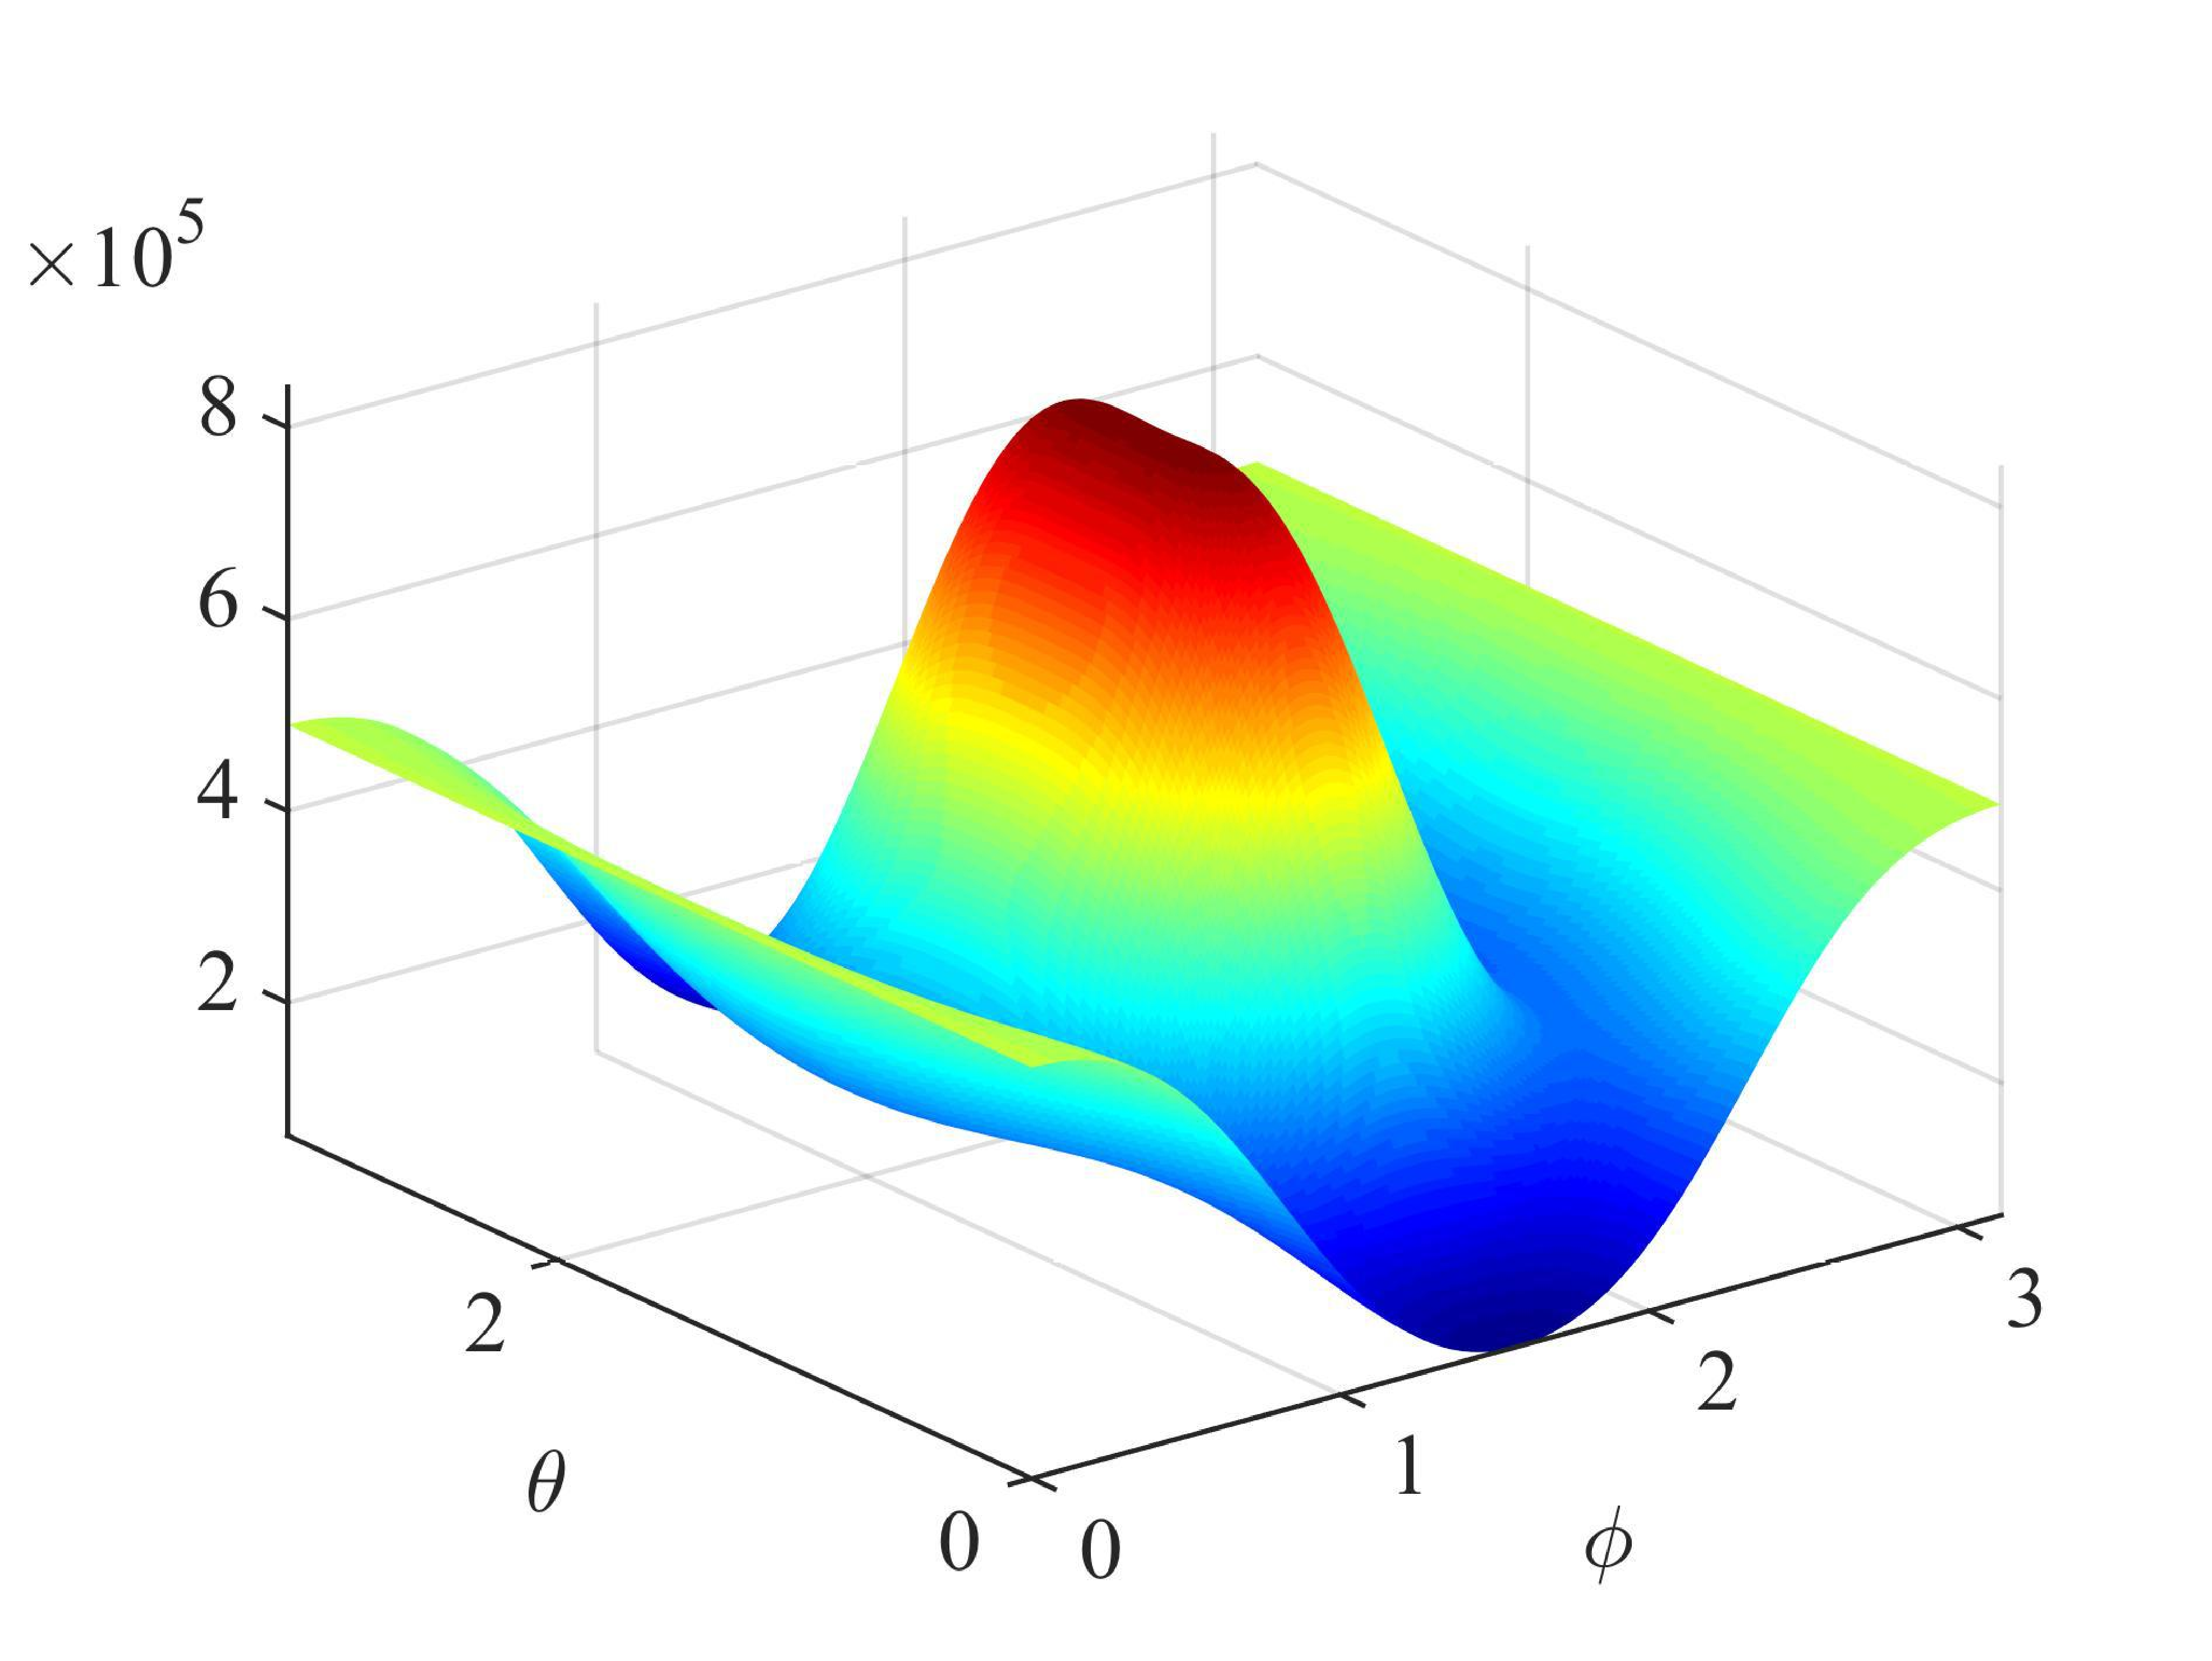
\includegraphics[width=0.45\textwidth]
   {figs/aniso_uniaxial_spherical_detA_F1p0762.pdf}
 } \subfigure[$F_{11}=1.1583$]{
   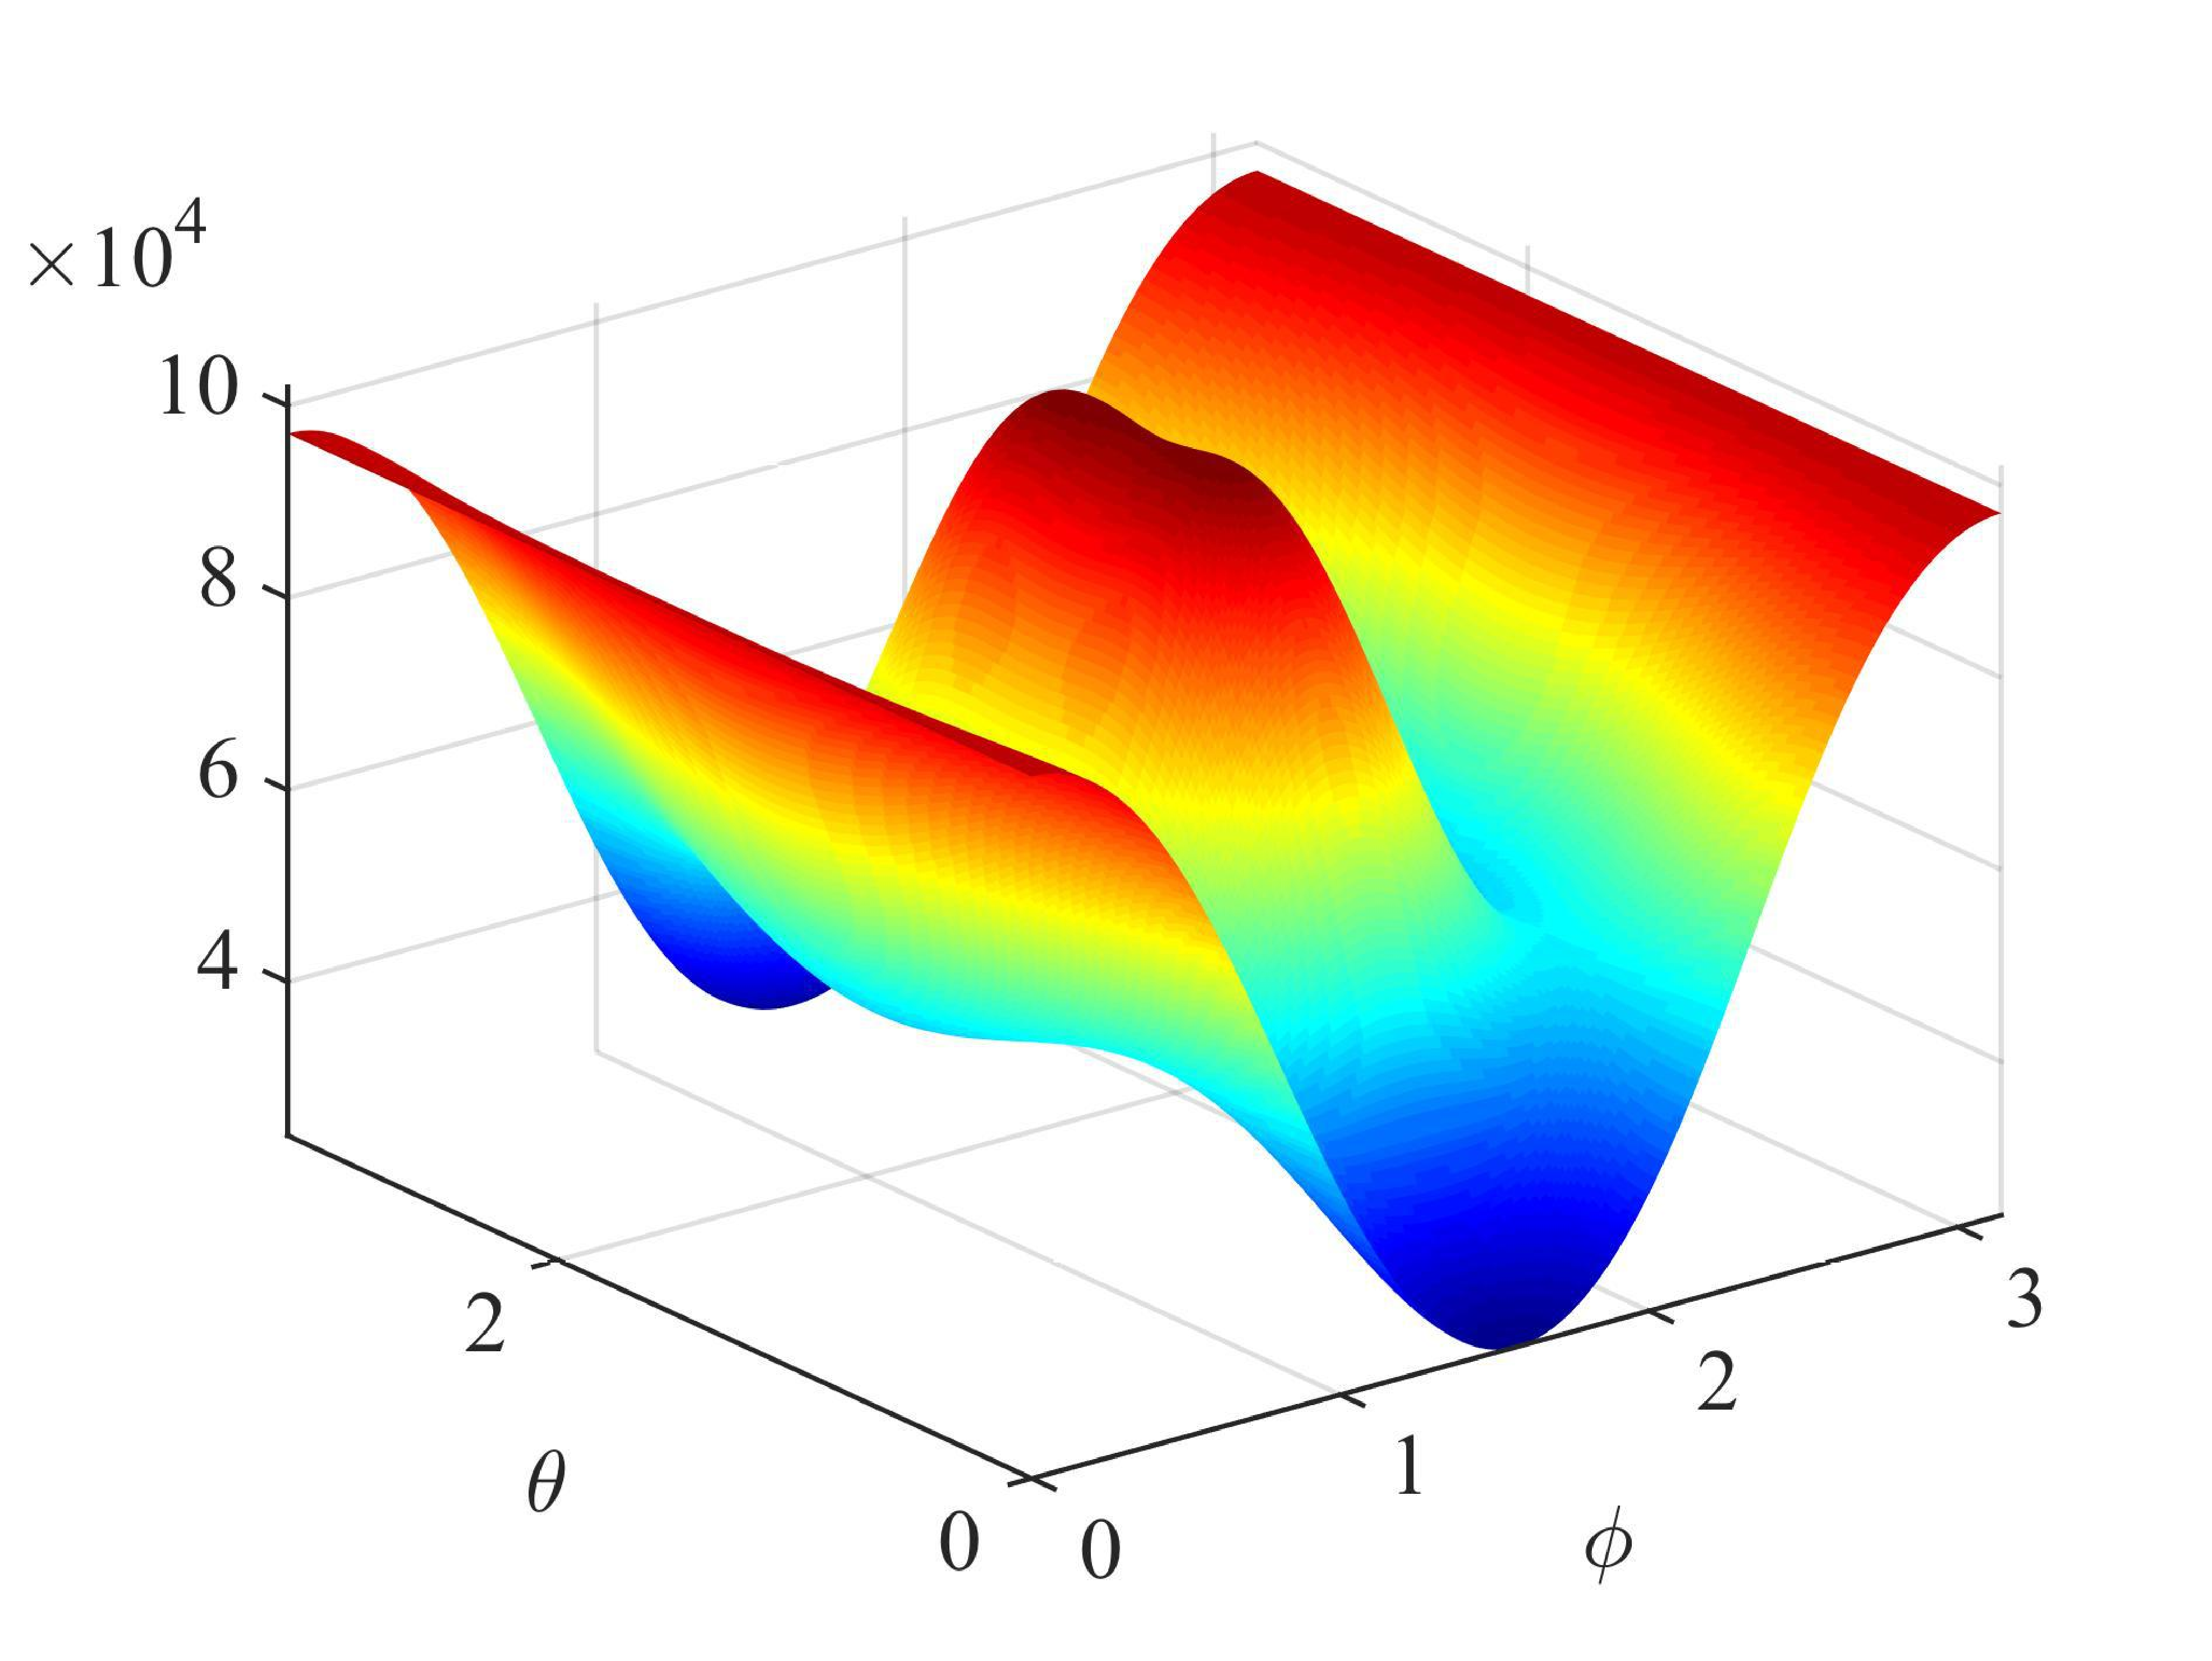
\includegraphics[width=0.45\textwidth]
   {figs/aniso_uniaxial_spherical_detA_F1p1583.pdf}
 } \subfigure[$F_{11}=1.1954$ (bifurcation)]{
   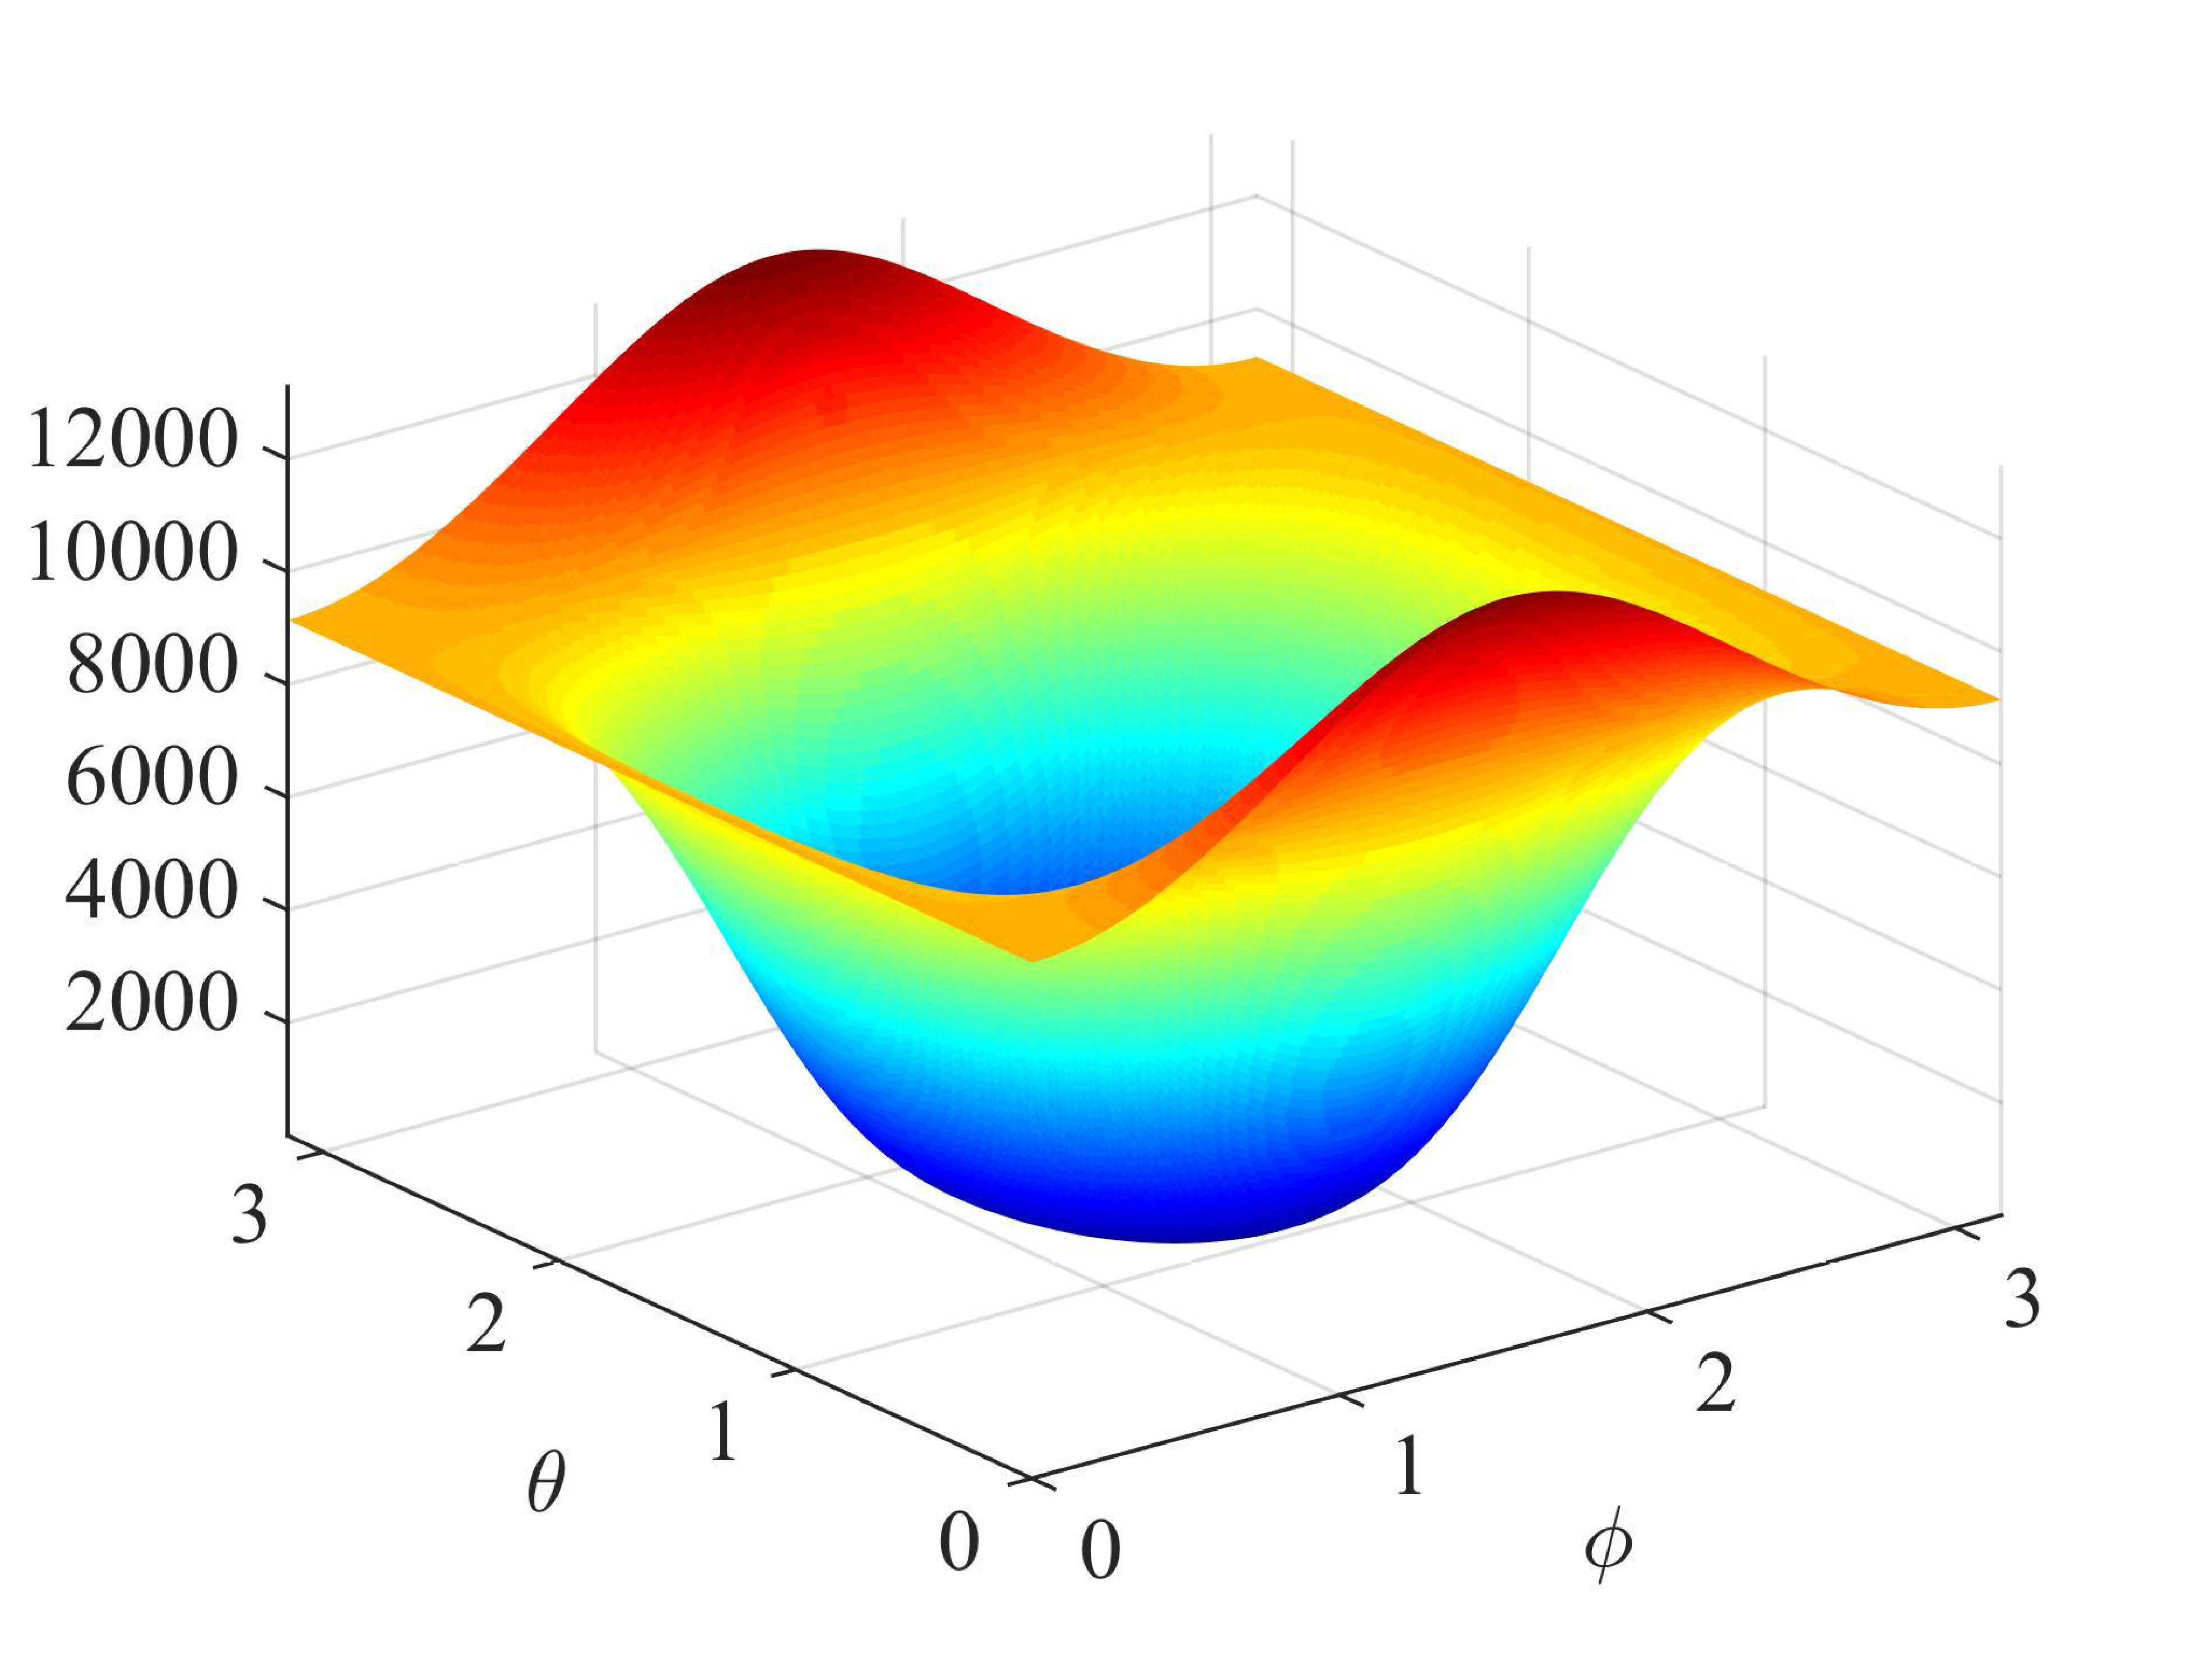
\includegraphics[width=0.45\textwidth]
   {figs/aniso_uniaxial_spherical_detA_F1p1954.pdf}
 }
   \caption{Spherical parametrization: landscapes of det$\bA$ 
   for uniaxial tension test on finite deformation anisotropic model at
   different axial stretch levels.}
   \label{fig:aniso_spherical_detA}
 \end{figure}

\begin{figure}[H]
   \centering \subfigure[$F_{11}=1.0074$]{
   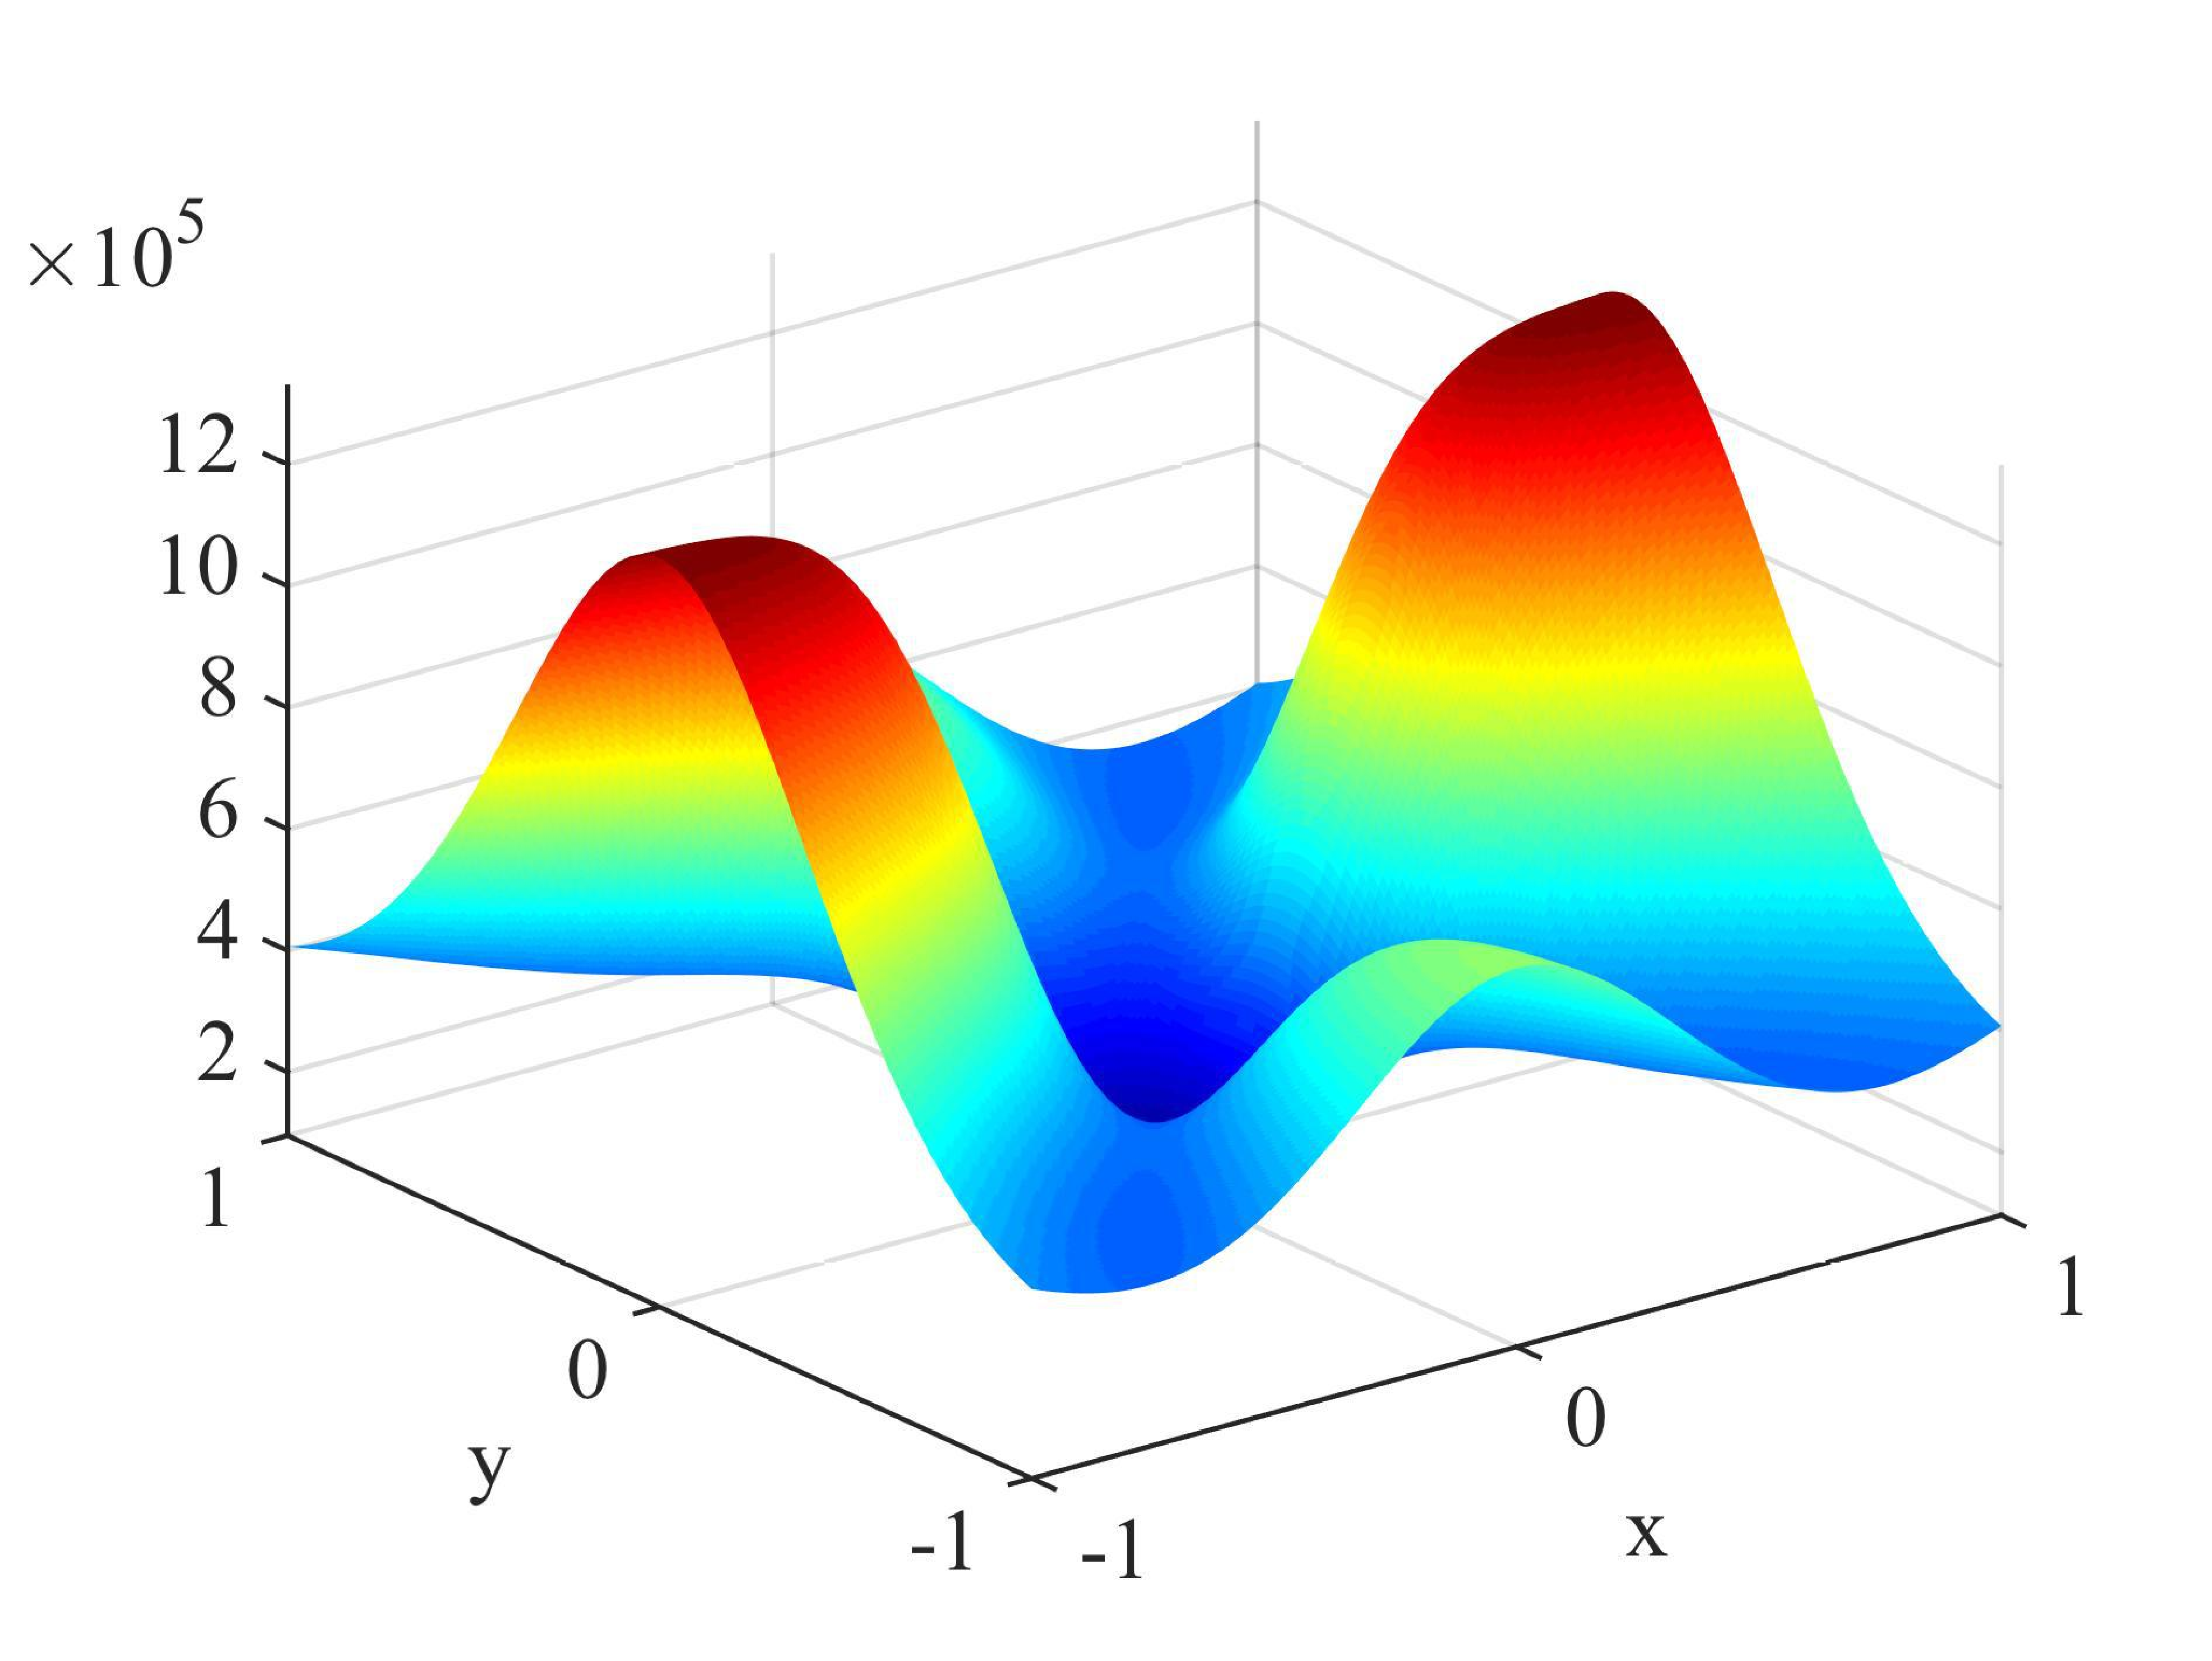
\includegraphics[width=0.45\textwidth]
   {figs/aniso_uniaxial_stereographic_detA_F1p0074.pdf}
 } \subfigure[$F_{11}=1.0762$]{
   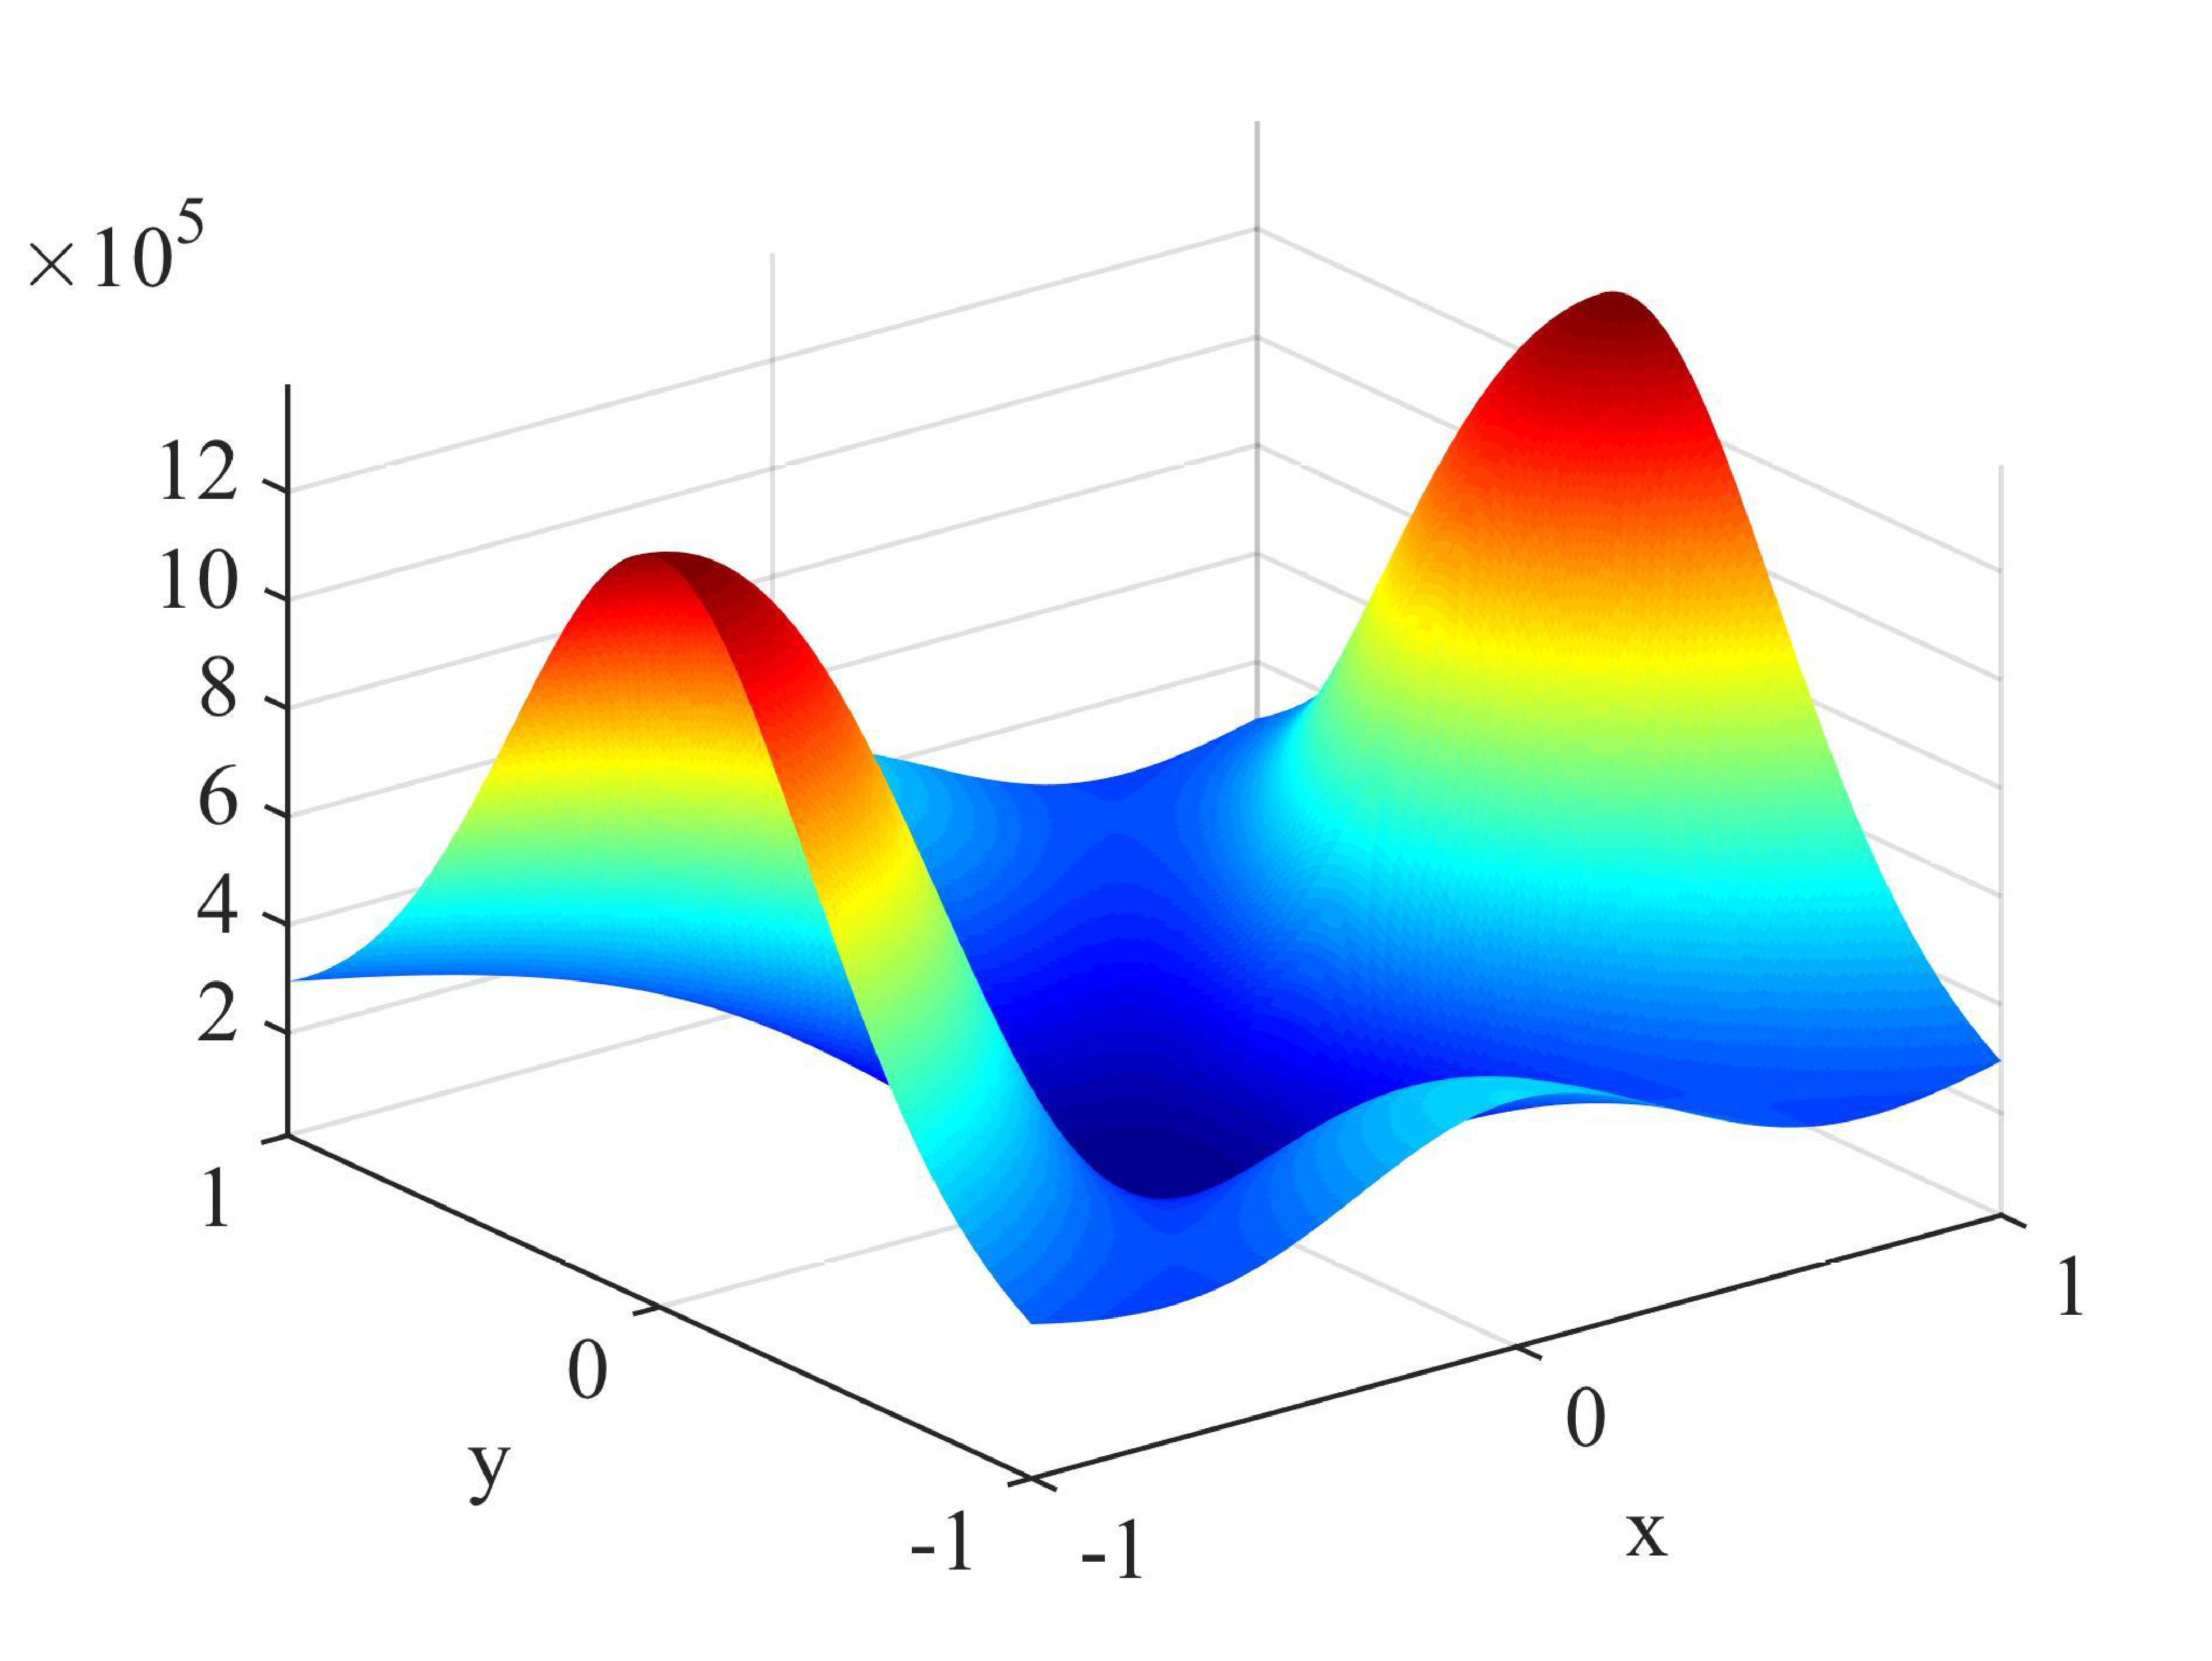
\includegraphics[width=0.45\textwidth]
   {figs/aniso_uniaxial_stereographic_detA_F1p0762.pdf}
 } \subfigure[$F_{11}=1.1583$]{
   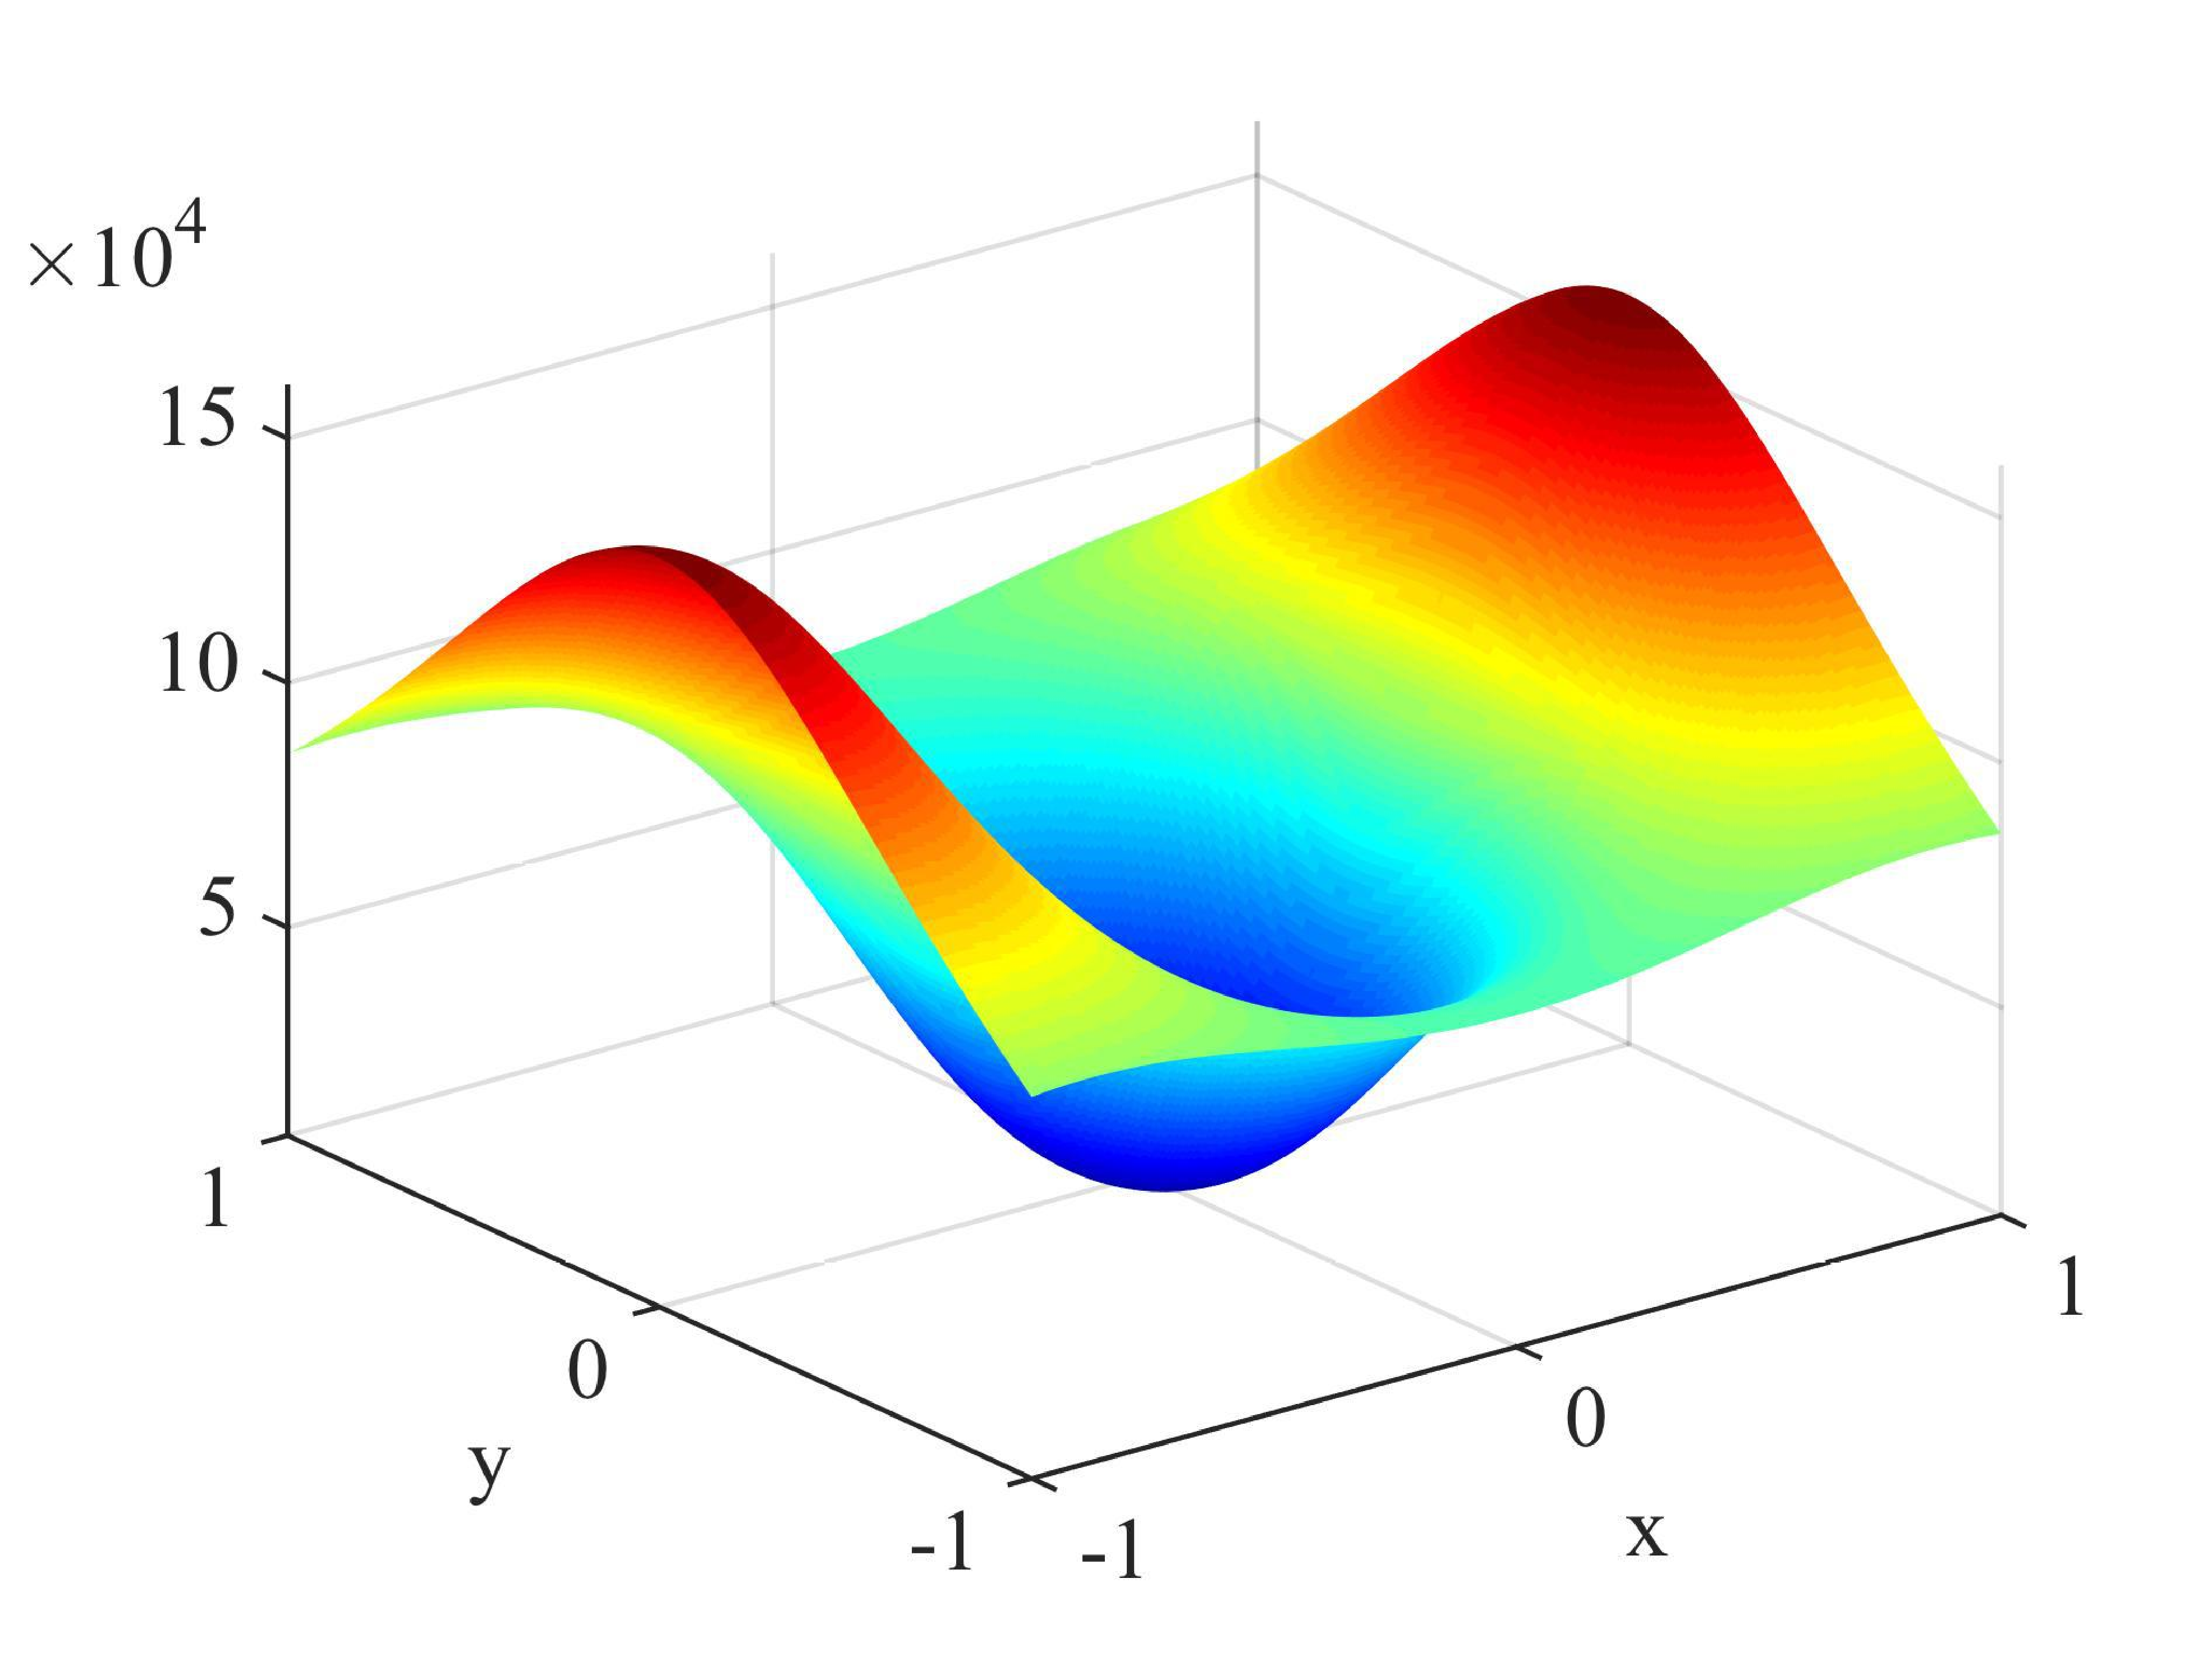
\includegraphics[width=0.45\textwidth]
   {figs/aniso_uniaxial_stereographic_detA_F1p1583.pdf}
 } \subfigure[$F_{11}=1.1954$ (bifurcation)]{
   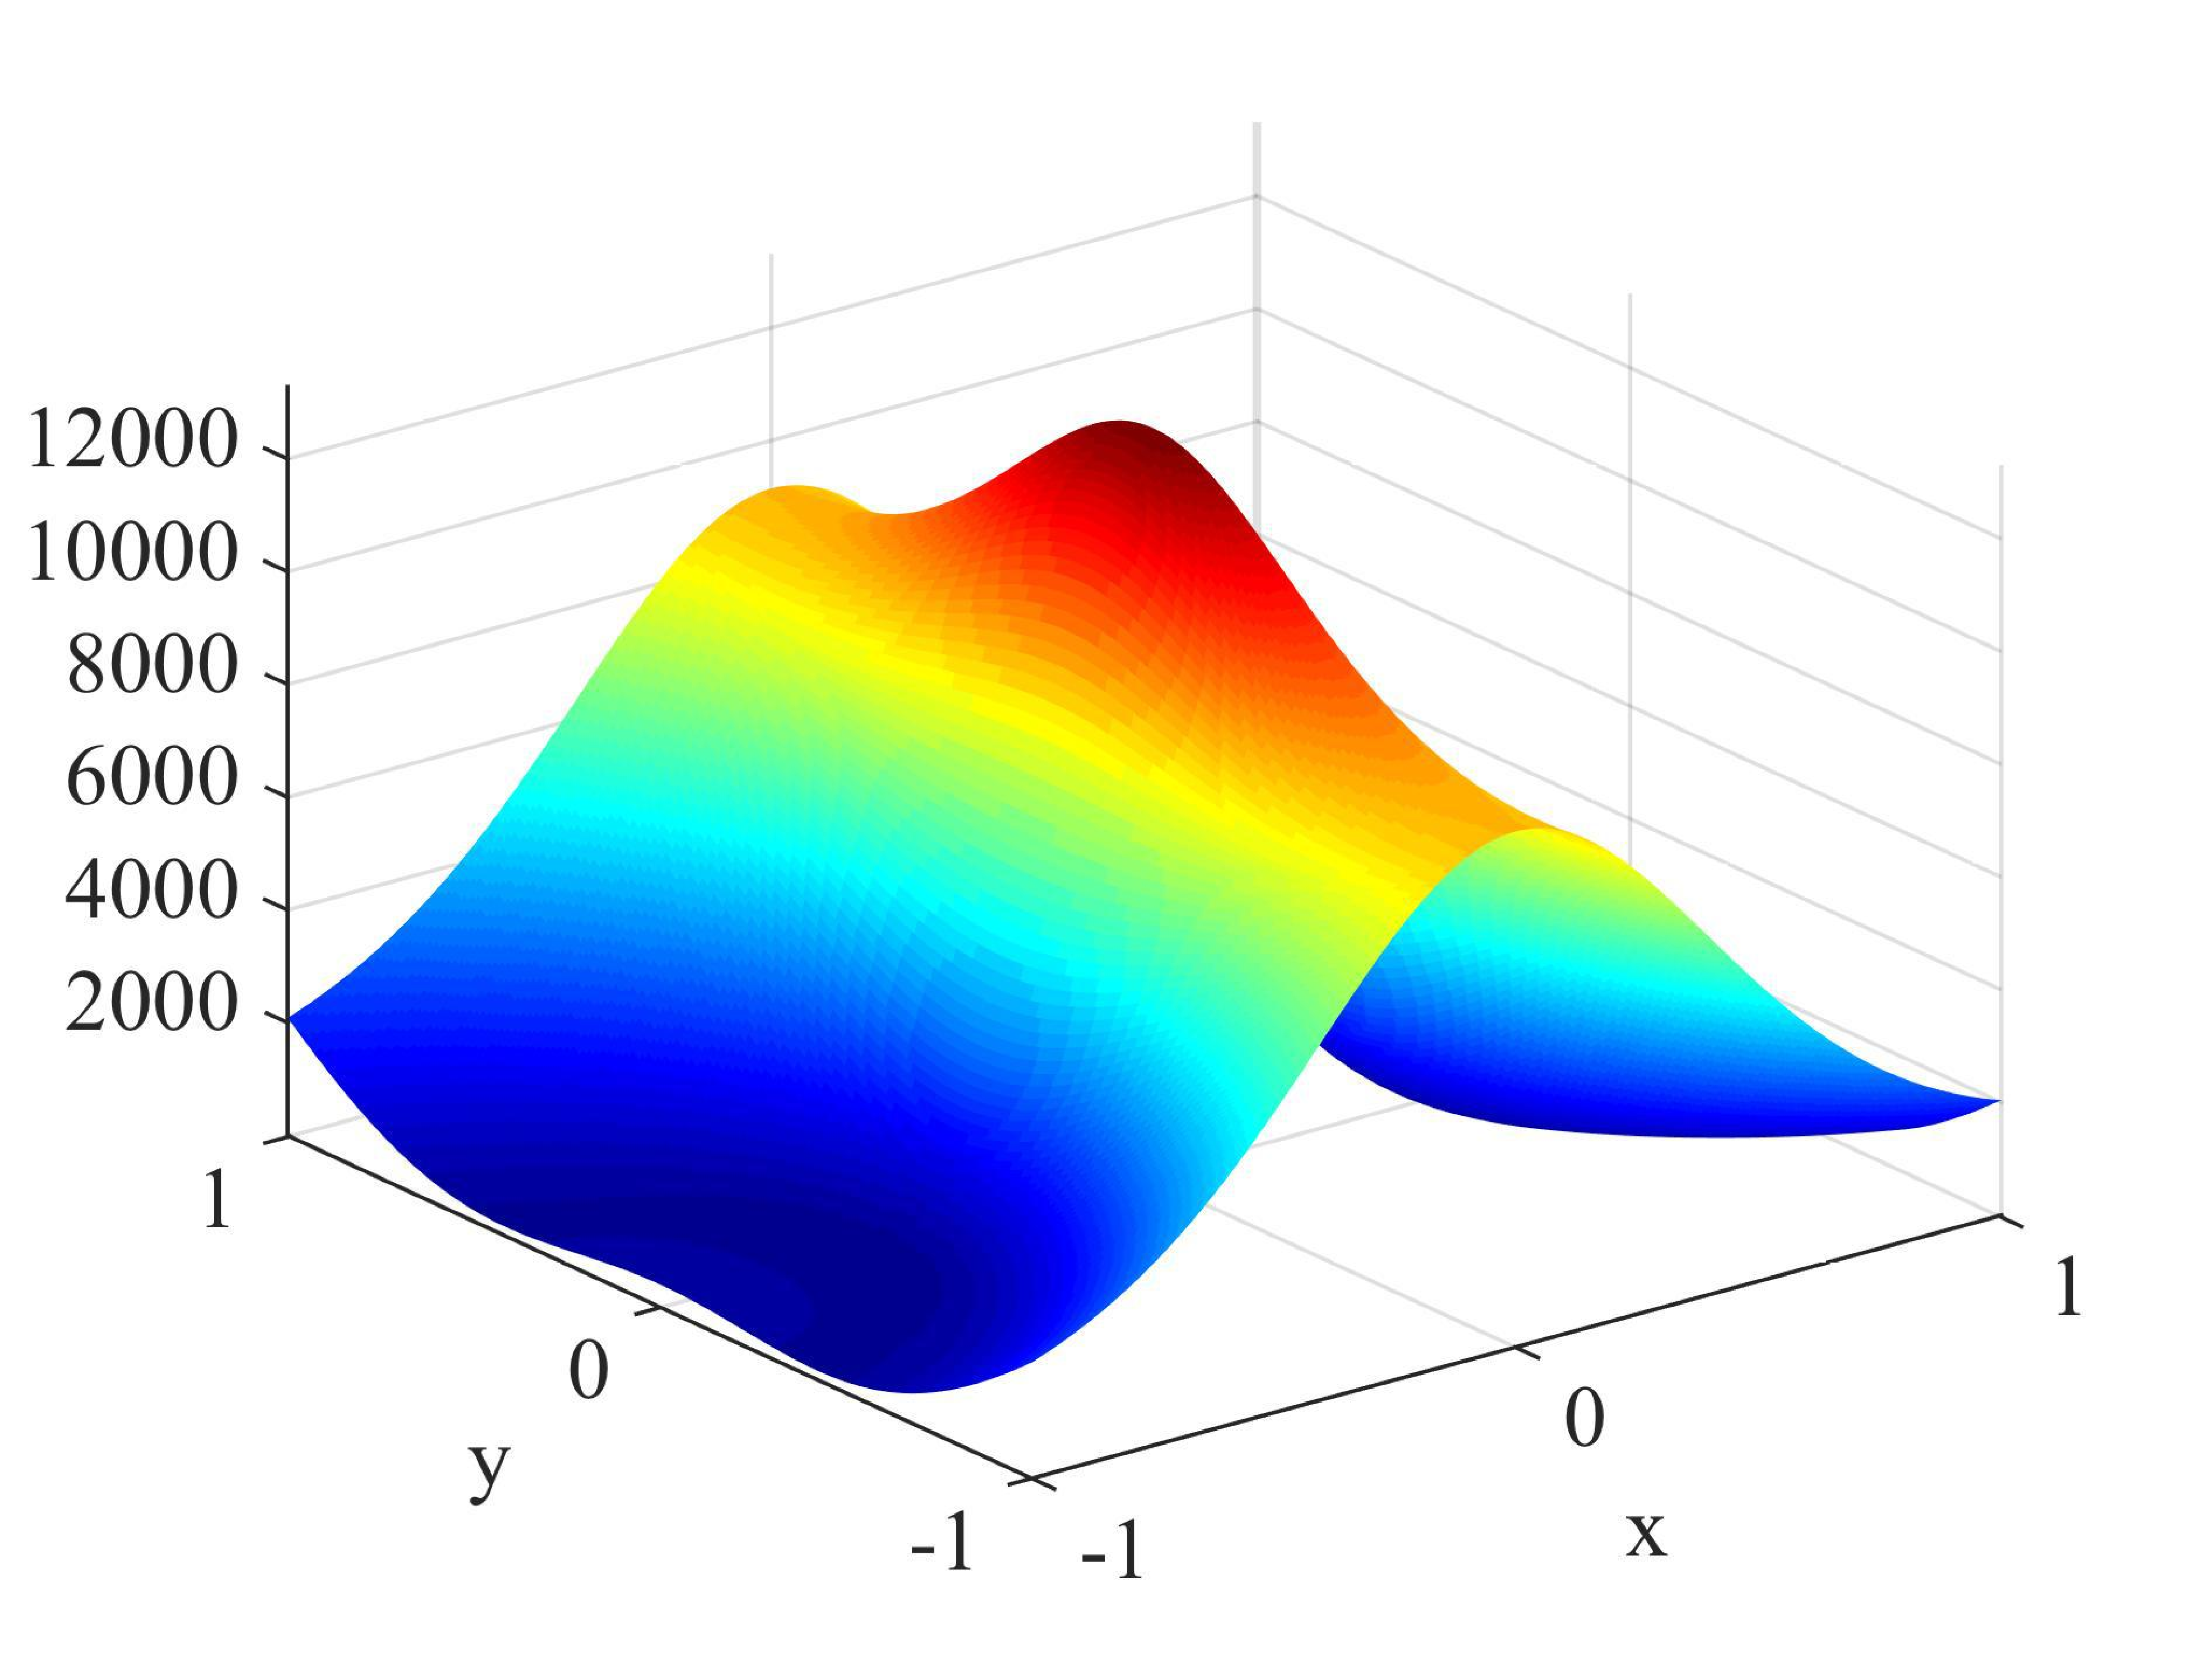
\includegraphics[width=0.45\textwidth]
   {figs/aniso_uniaxial_stereographic_detA_F1p1954.pdf}
 }
   \caption{Stereographic parametrization: landscapes of det$\bA$ 
   for uniaxial tension test on finite deformation anisotropic model at
   different axial stretch levels.}
   \label{fig:aniso_stereographic_detA}
 \end{figure}

\begin{figure}[H]
   \centering \subfigure[$F_{11}=1.0074$]{
   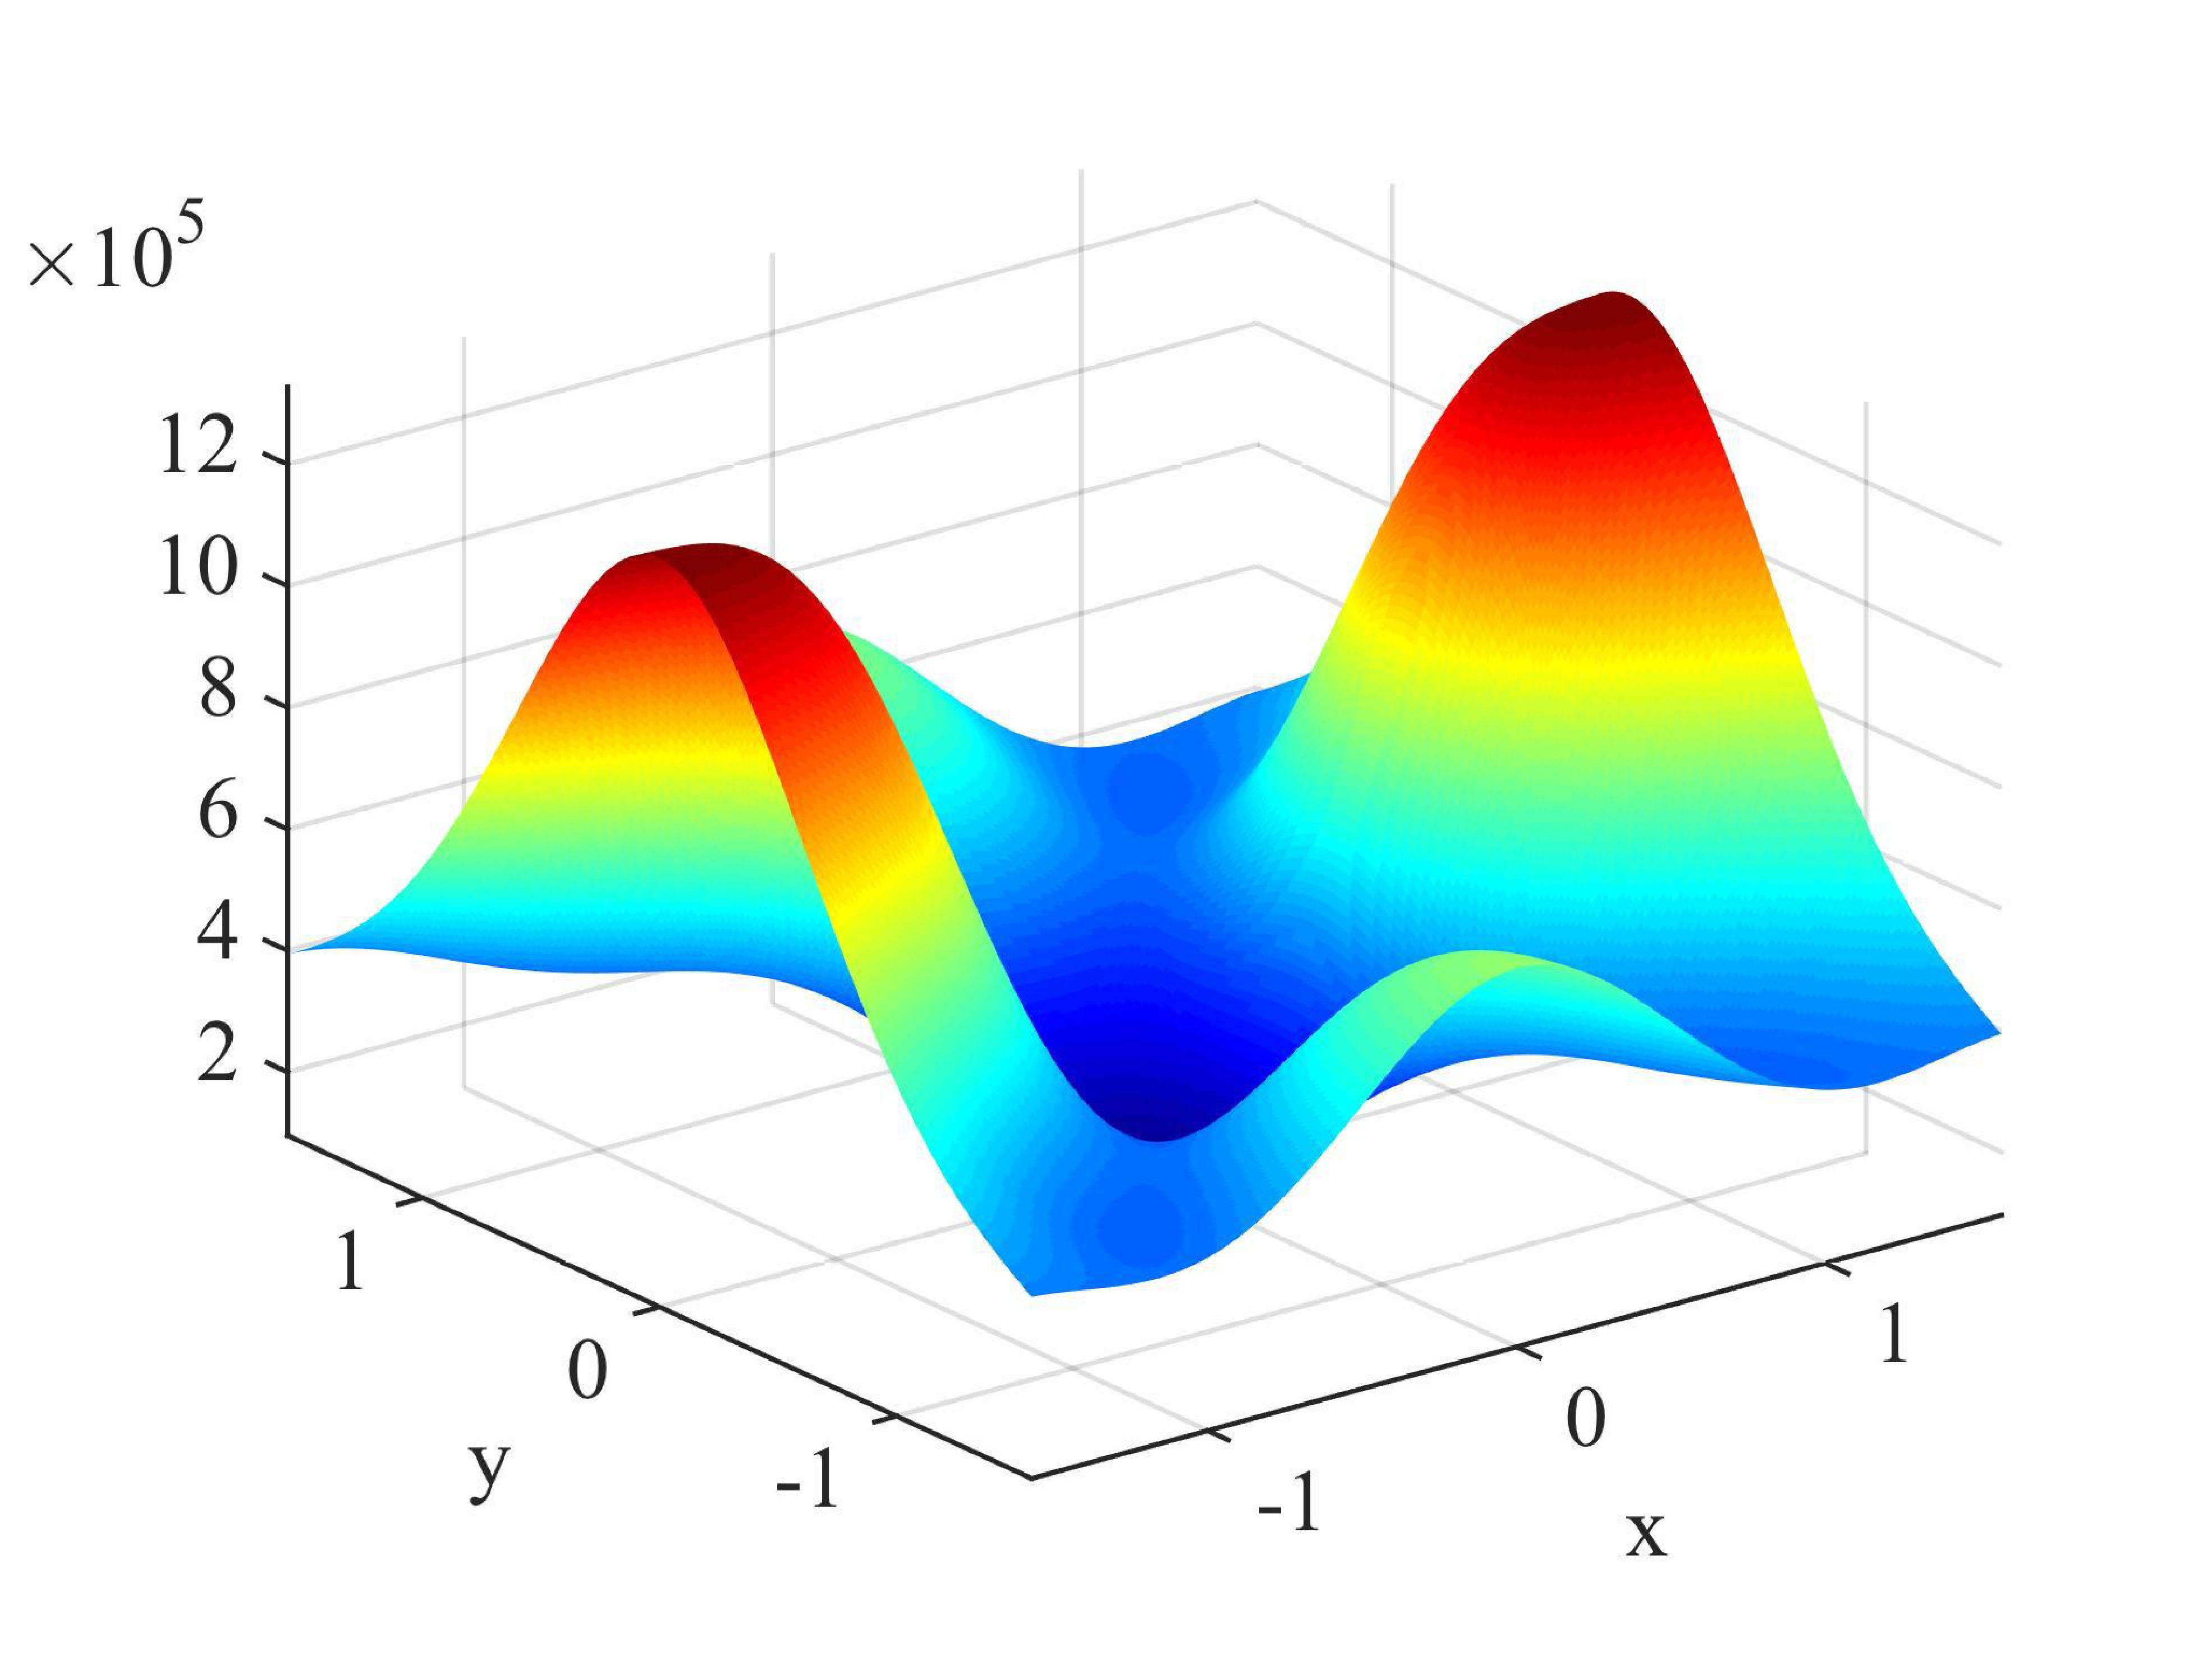
\includegraphics[width=0.45\textwidth]
   {figs/aniso_uniaxial_tangent_detA_F1p0074.pdf}
 } \subfigure[$F_{11}=1.0762$]{
   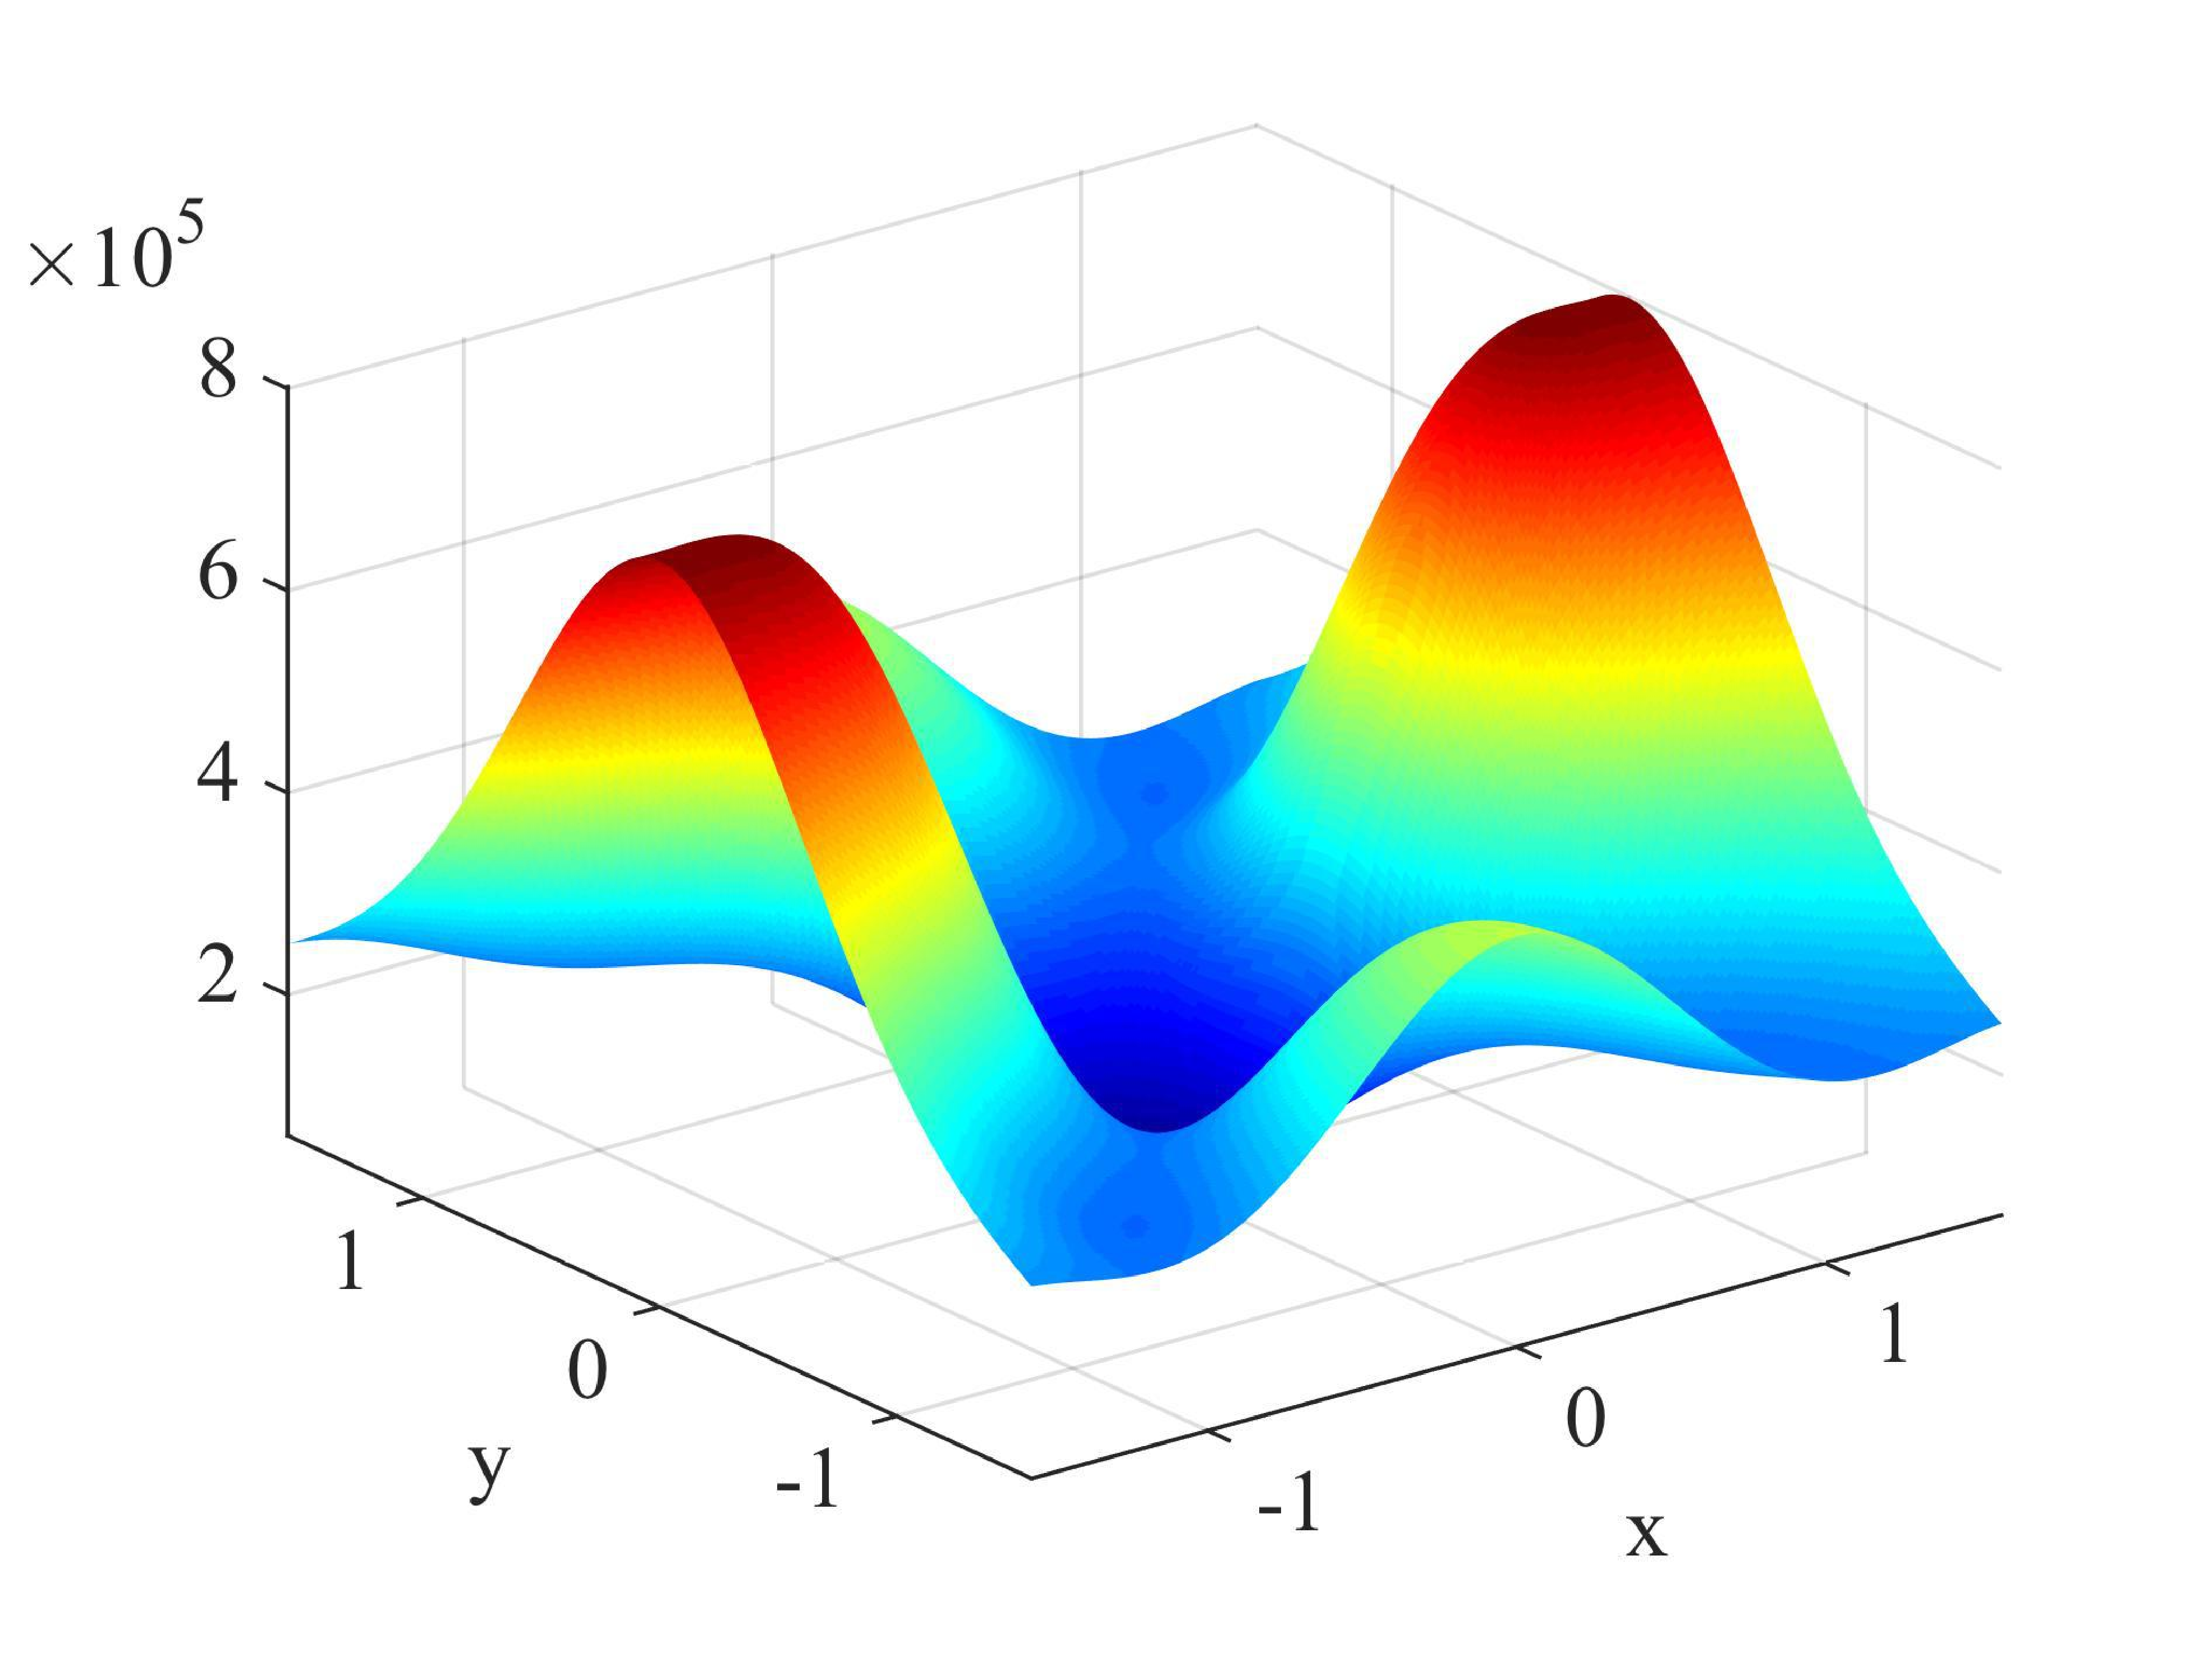
\includegraphics[width=0.45\textwidth]
   {figs/aniso_uniaxial_tangent_detA_F1p0762.pdf}
 } \subfigure[$F_{11}=1.1583$]{
   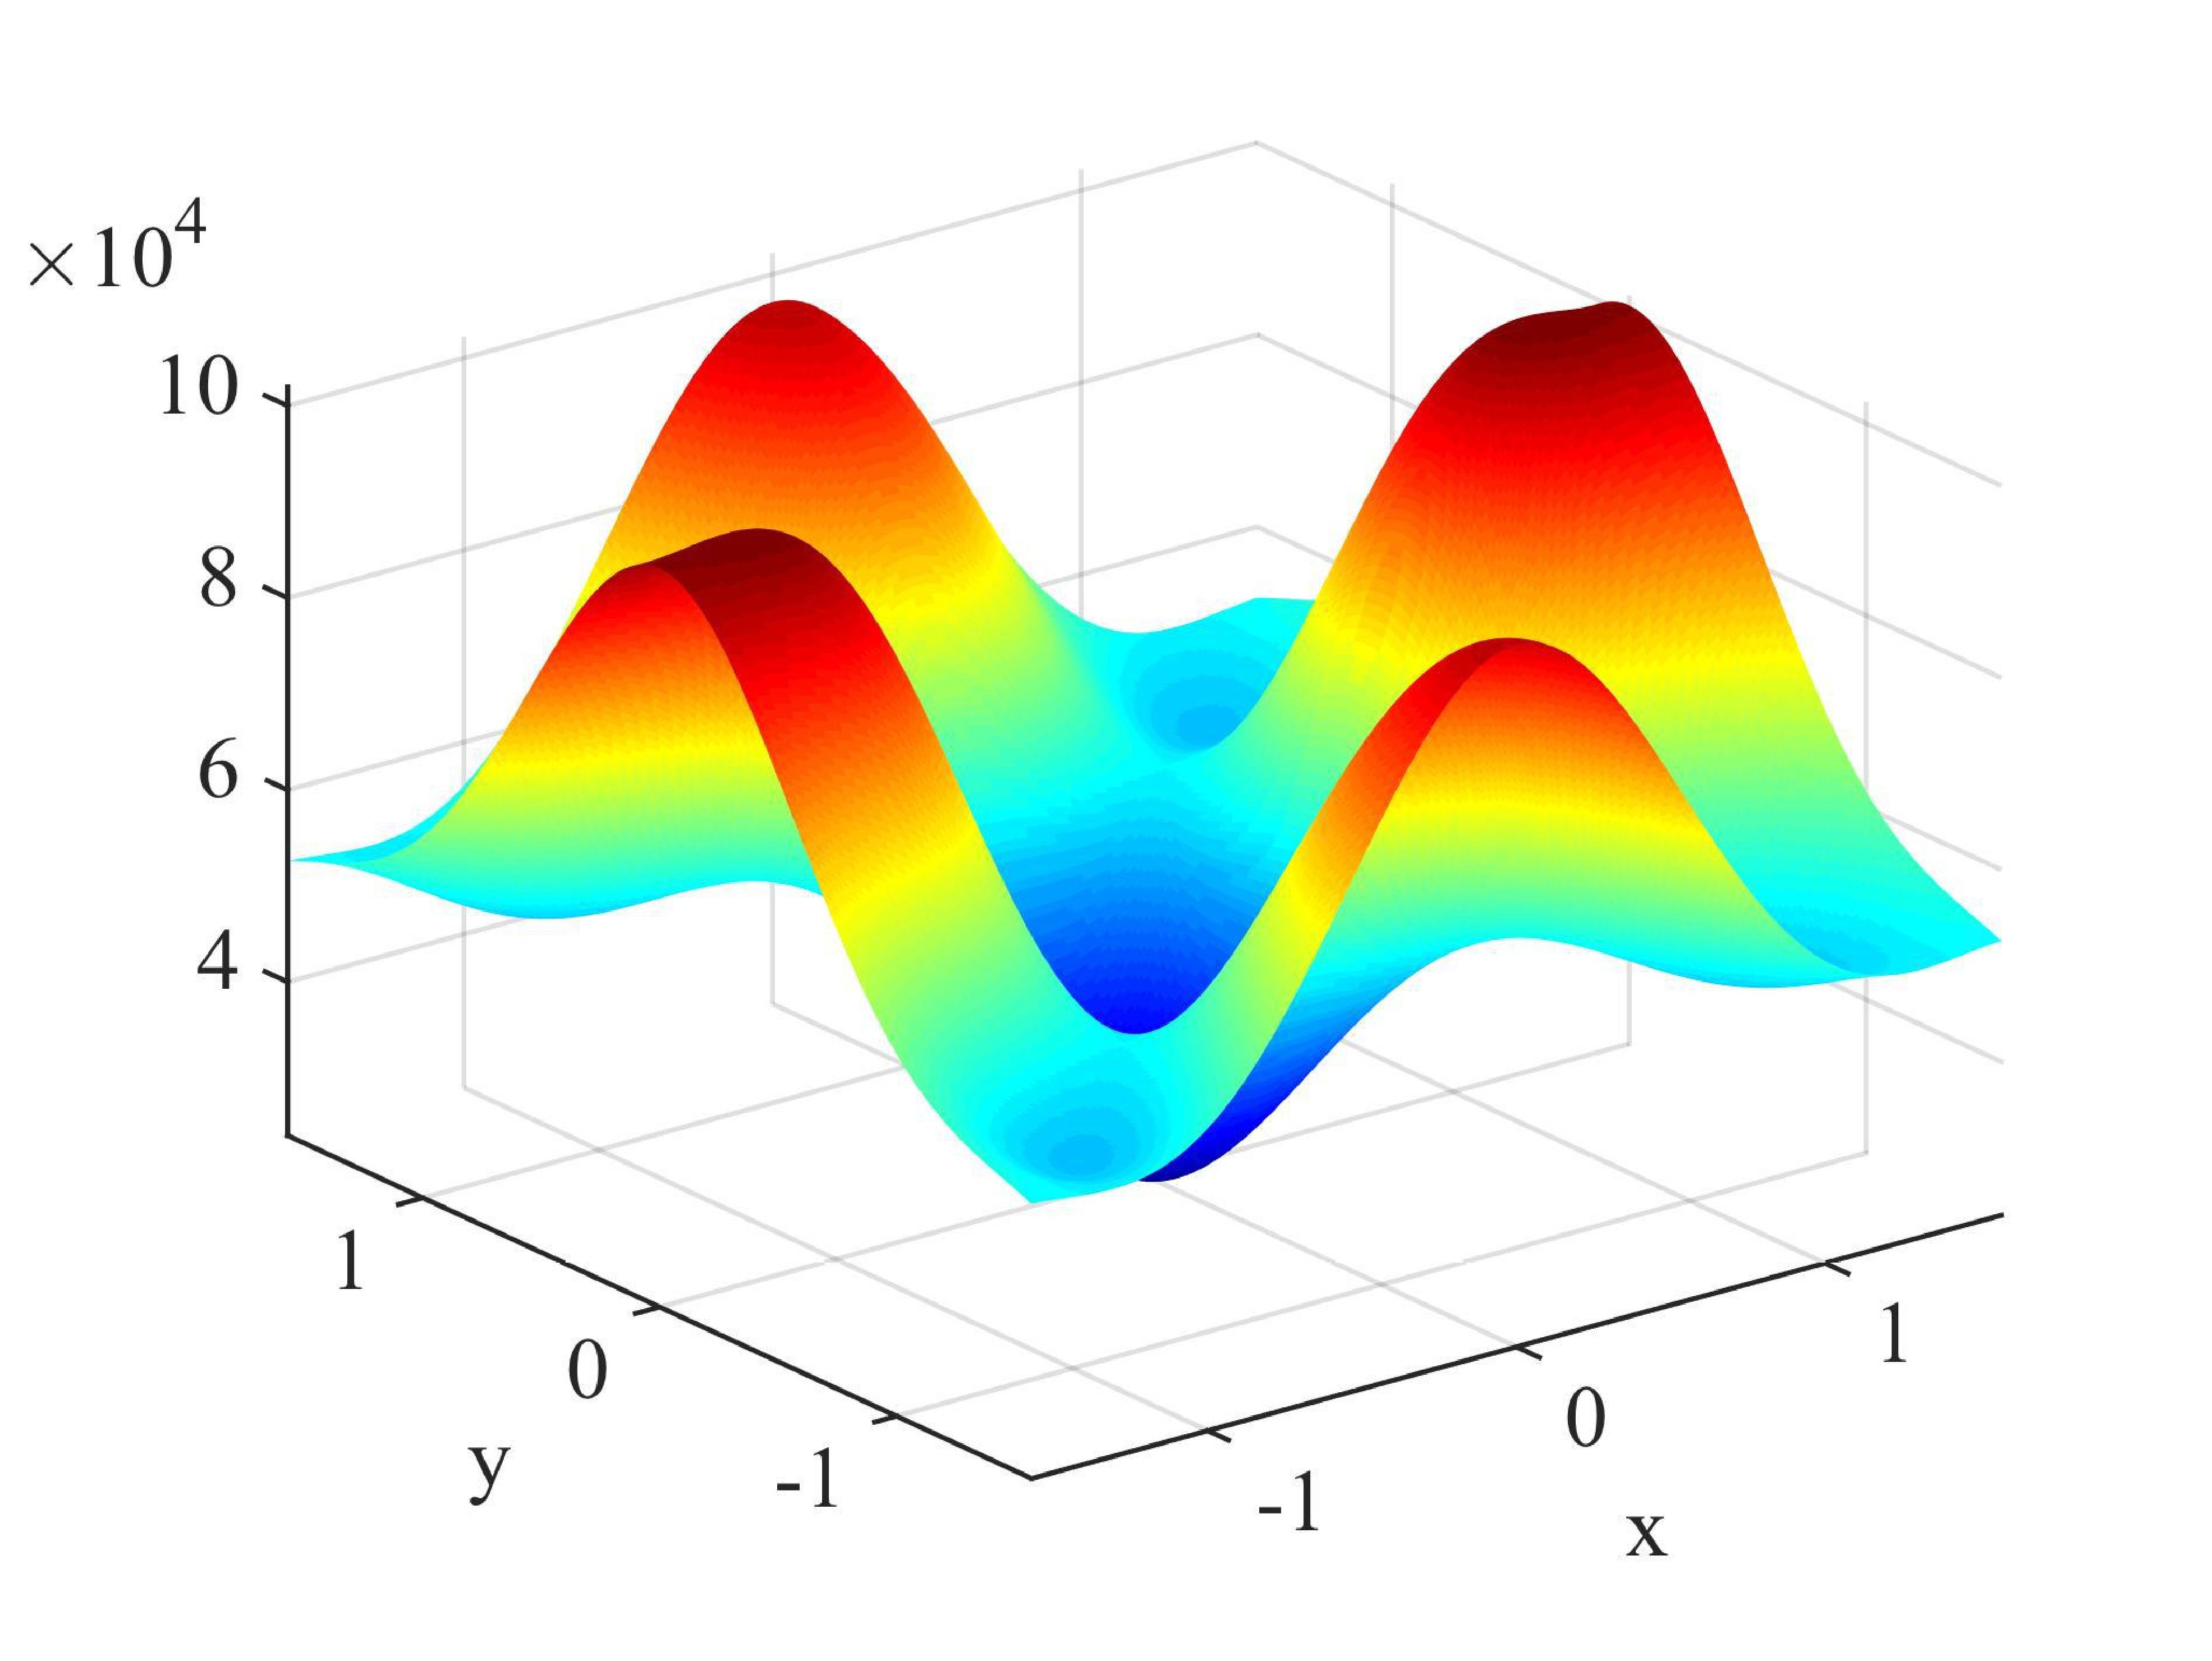
\includegraphics[width=0.45\textwidth]
   {figs/aniso_uniaxial_tangent_detA_F1p1583.pdf}
 } \subfigure[$F_{11}=1.1954$ (bifurcation)]{
   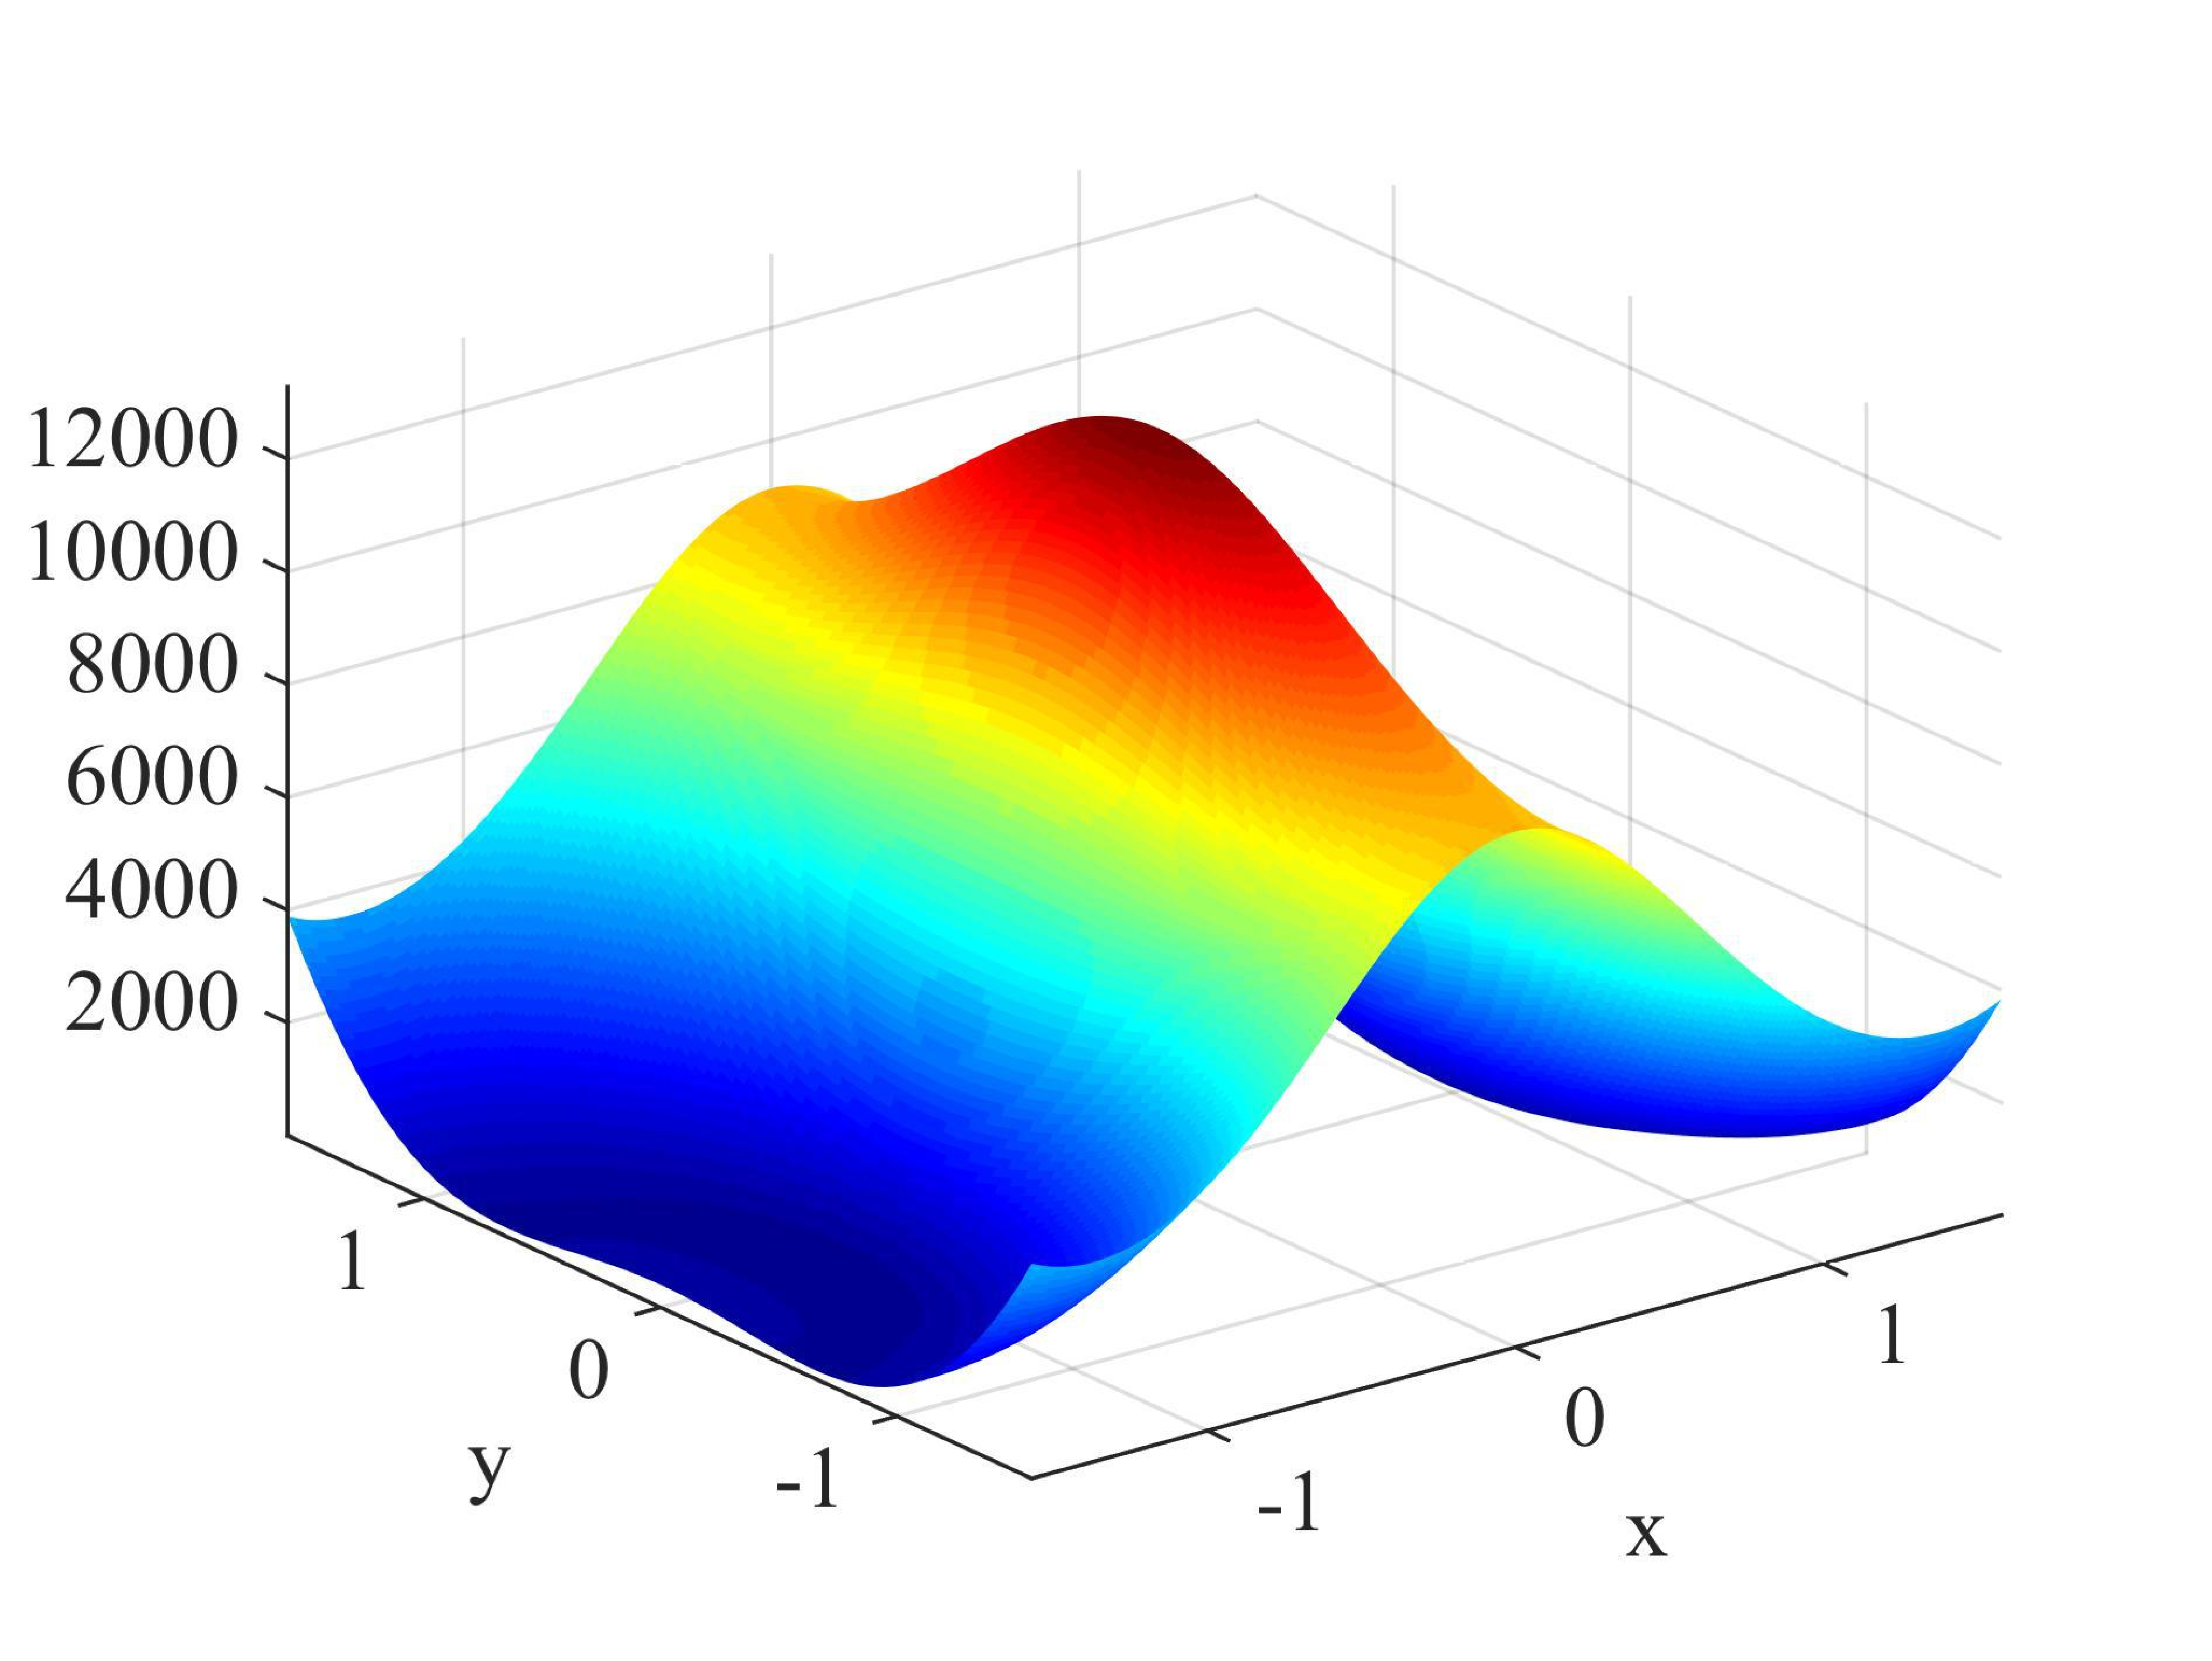
\includegraphics[width=0.45\textwidth]
   {figs/aniso_uniaxial_tangent_detA_F1p1954.pdf}
 }
   \caption{Tangent parametrization: landscapes of det$\bA$ 
   for uniaxial tension test on finite deformation anisotropic model at
   different axial stretch levels.}
   \label{fig:aniso_tangent_detA}
 \end{figure} 

\begin{figure}[H]
   \centering \subfigure[$F_{11}=1.0074$]{
   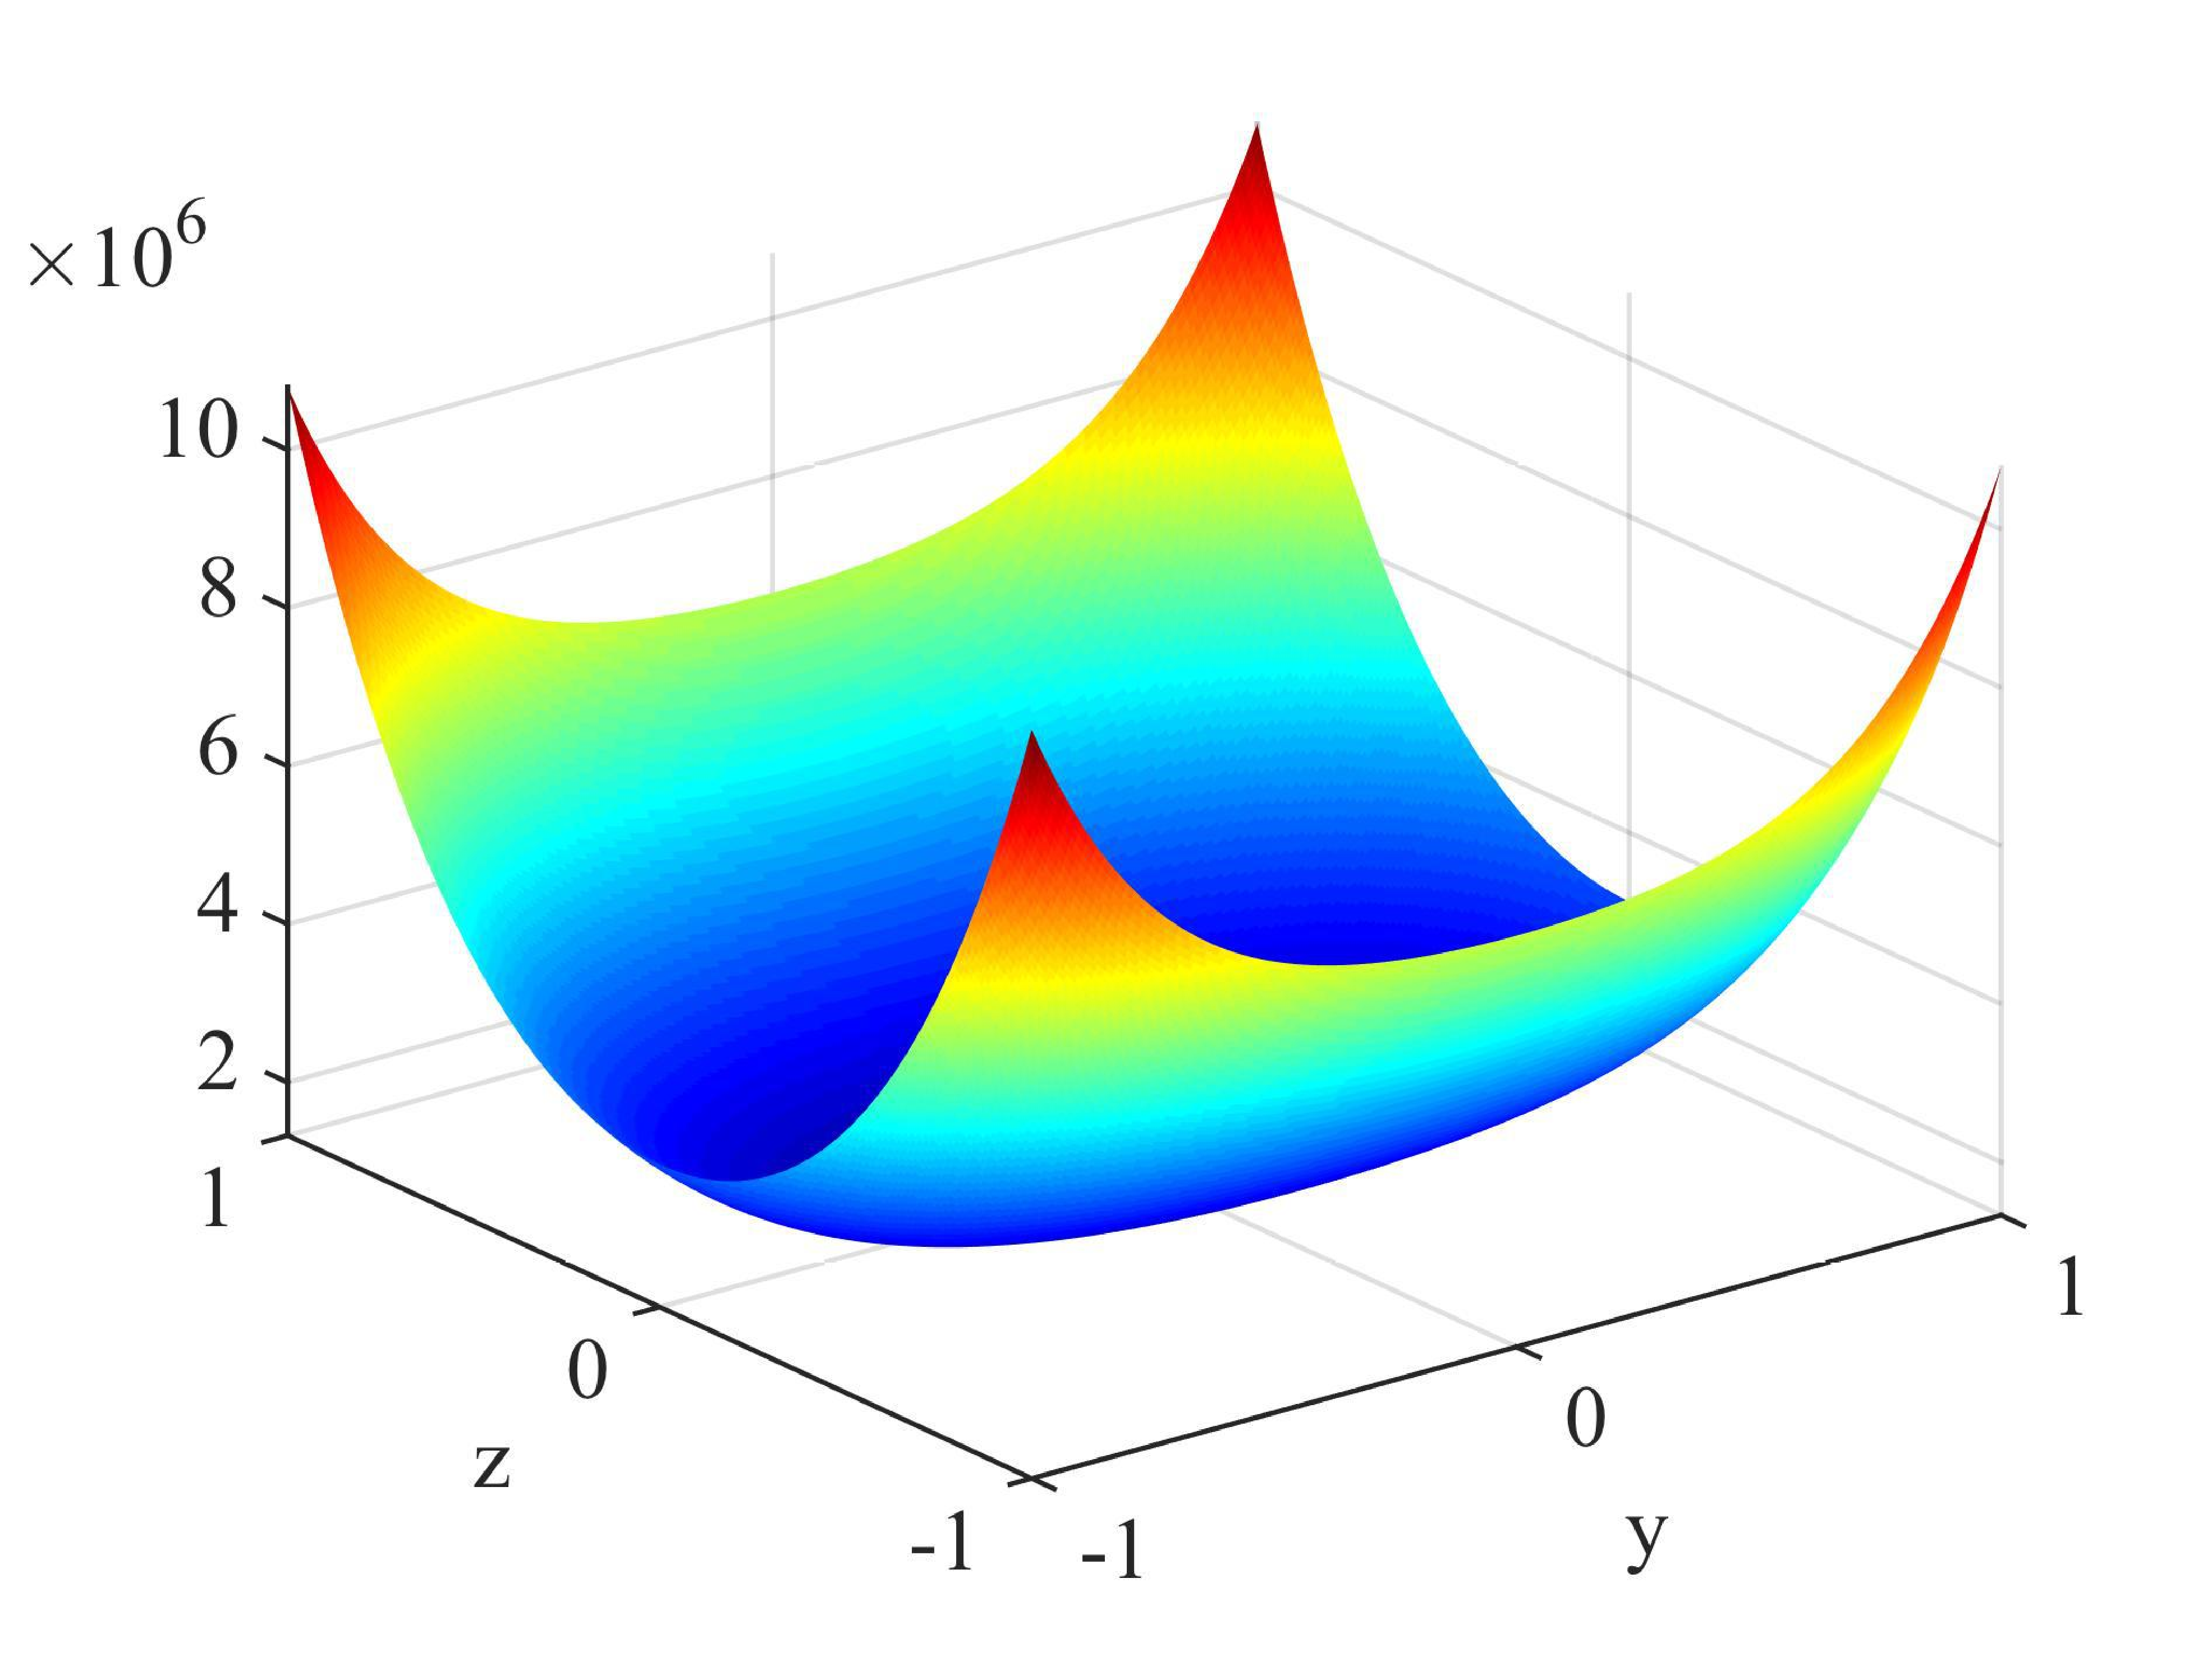
\includegraphics[width=0.45\textwidth]
   {figs/aniso_uniaxial_cartesian_detA_F1p0074.pdf}
 } \subfigure[$F_{11}=1.0762$]{
   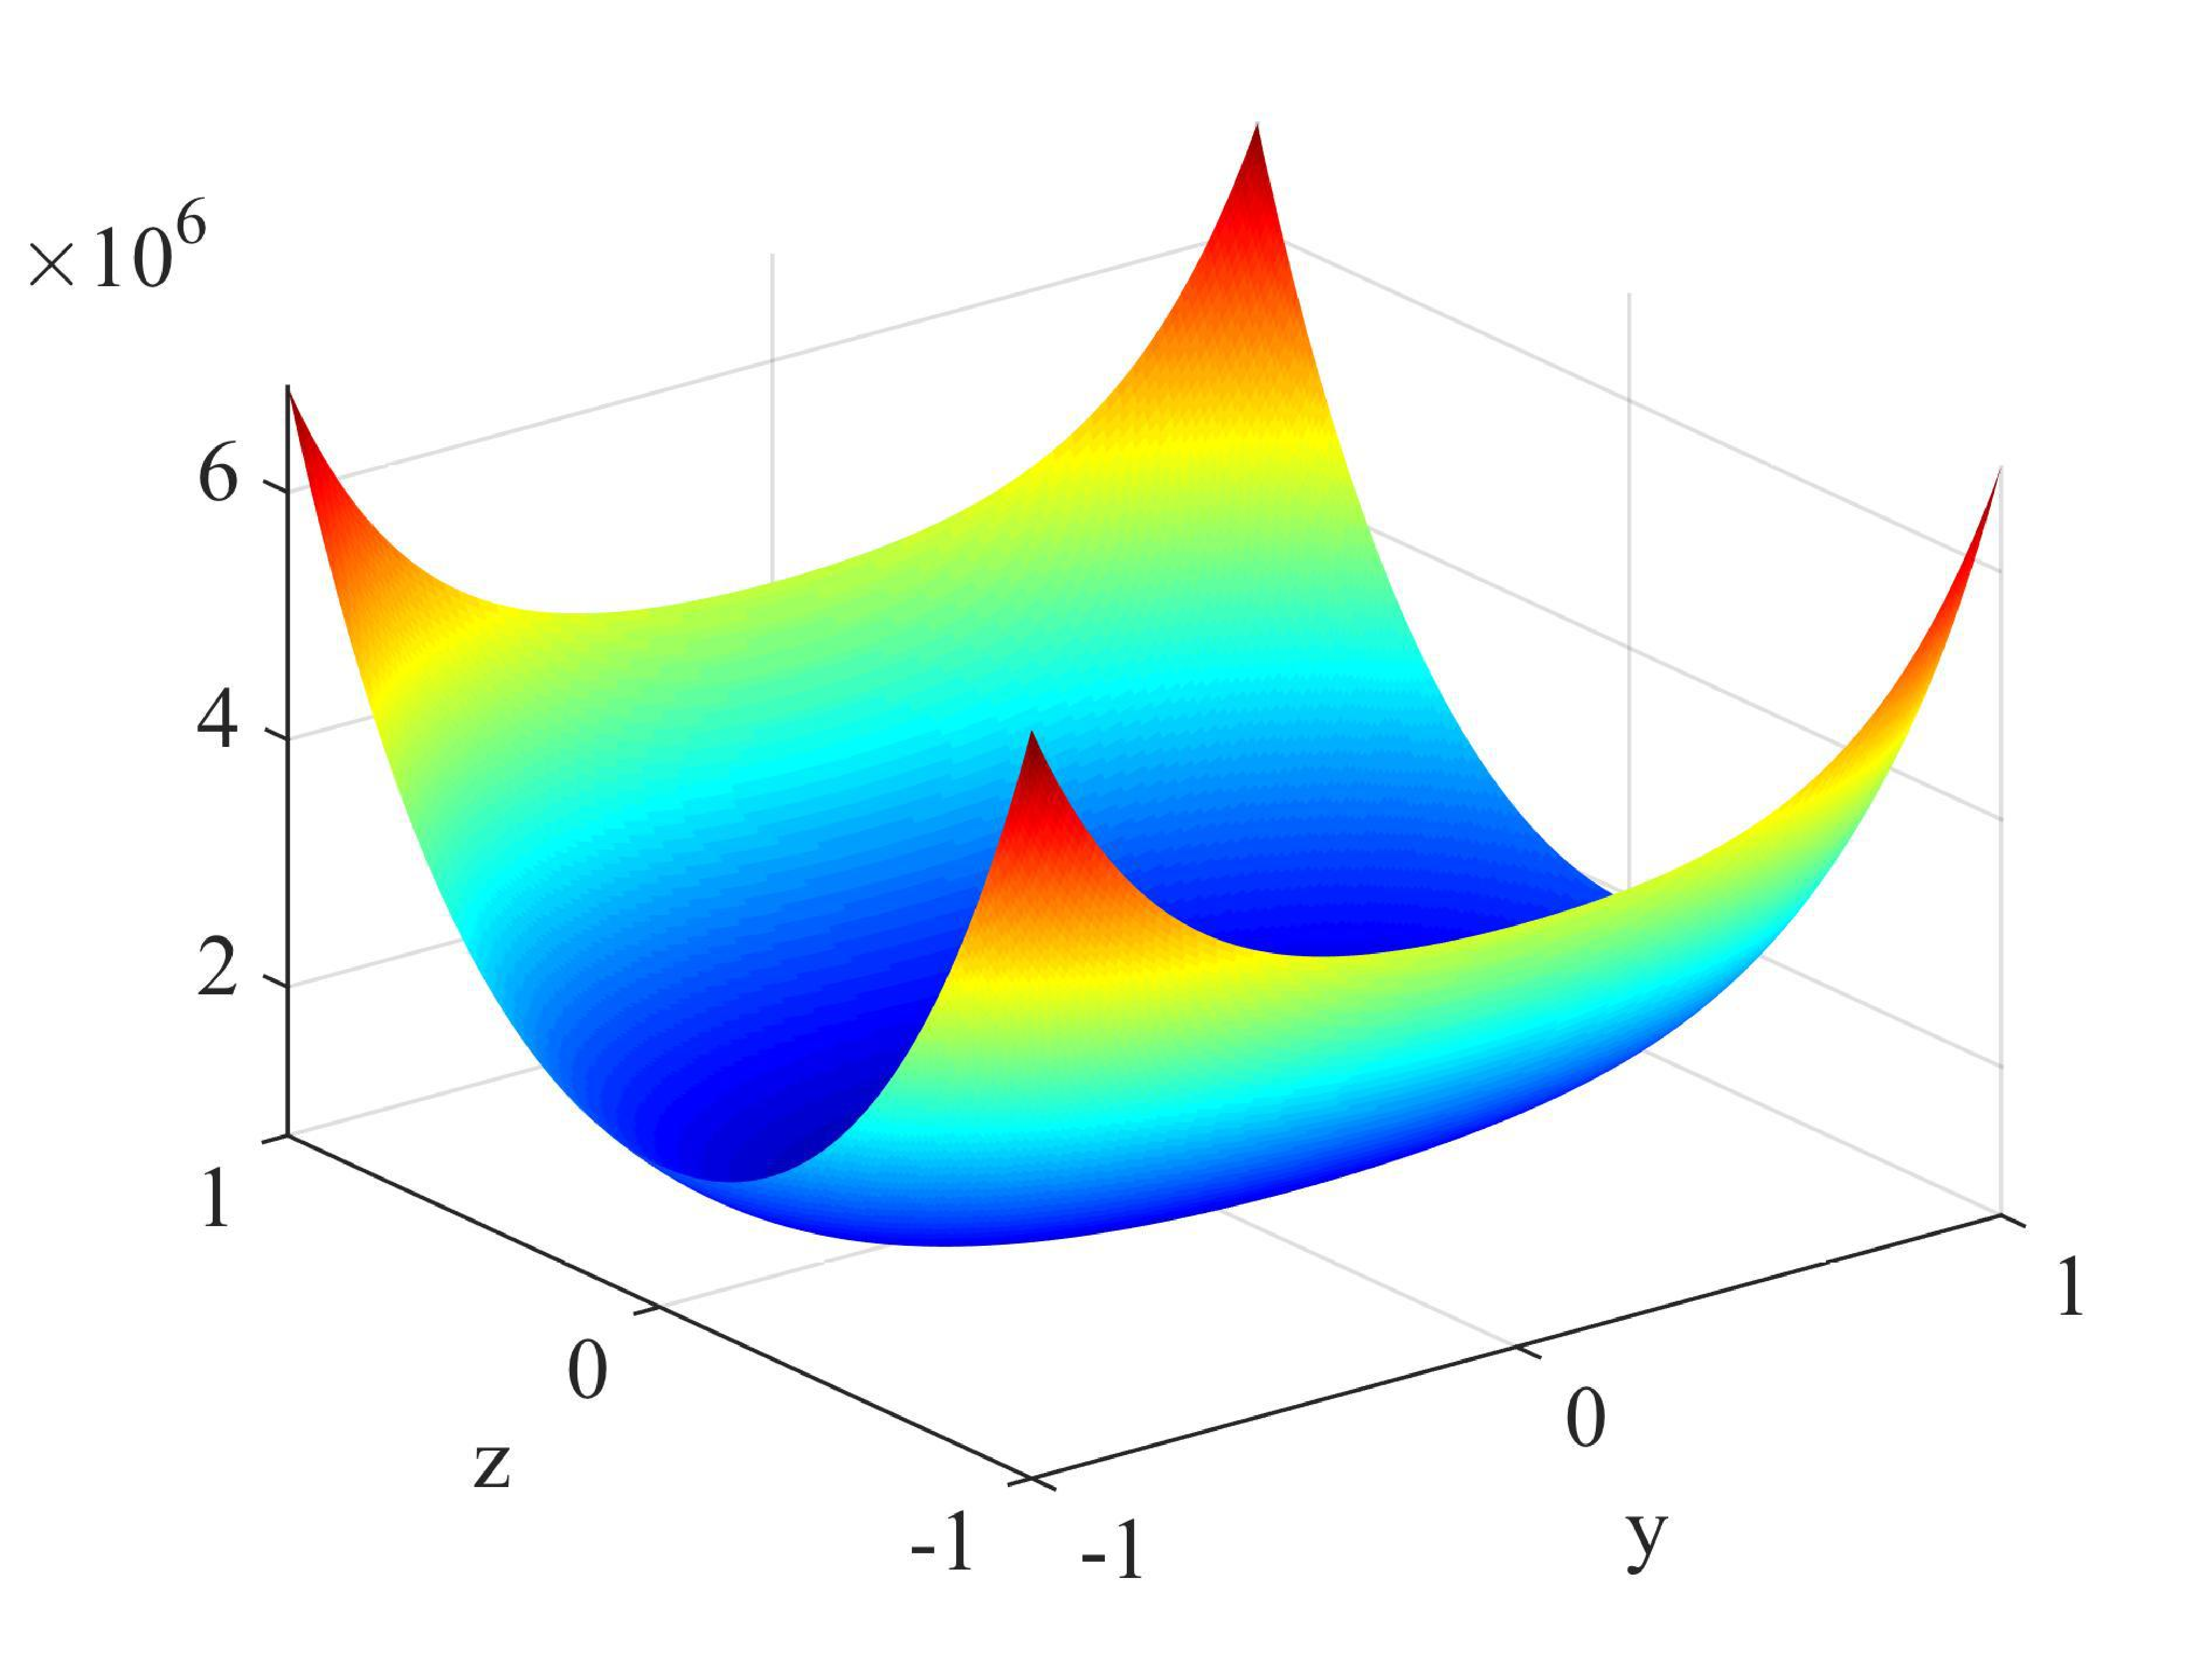
\includegraphics[width=0.45\textwidth]
   {figs/aniso_uniaxial_cartesian_detA_F1p0762.pdf}
 } \subfigure[$F_{11}=1.1583$]{
   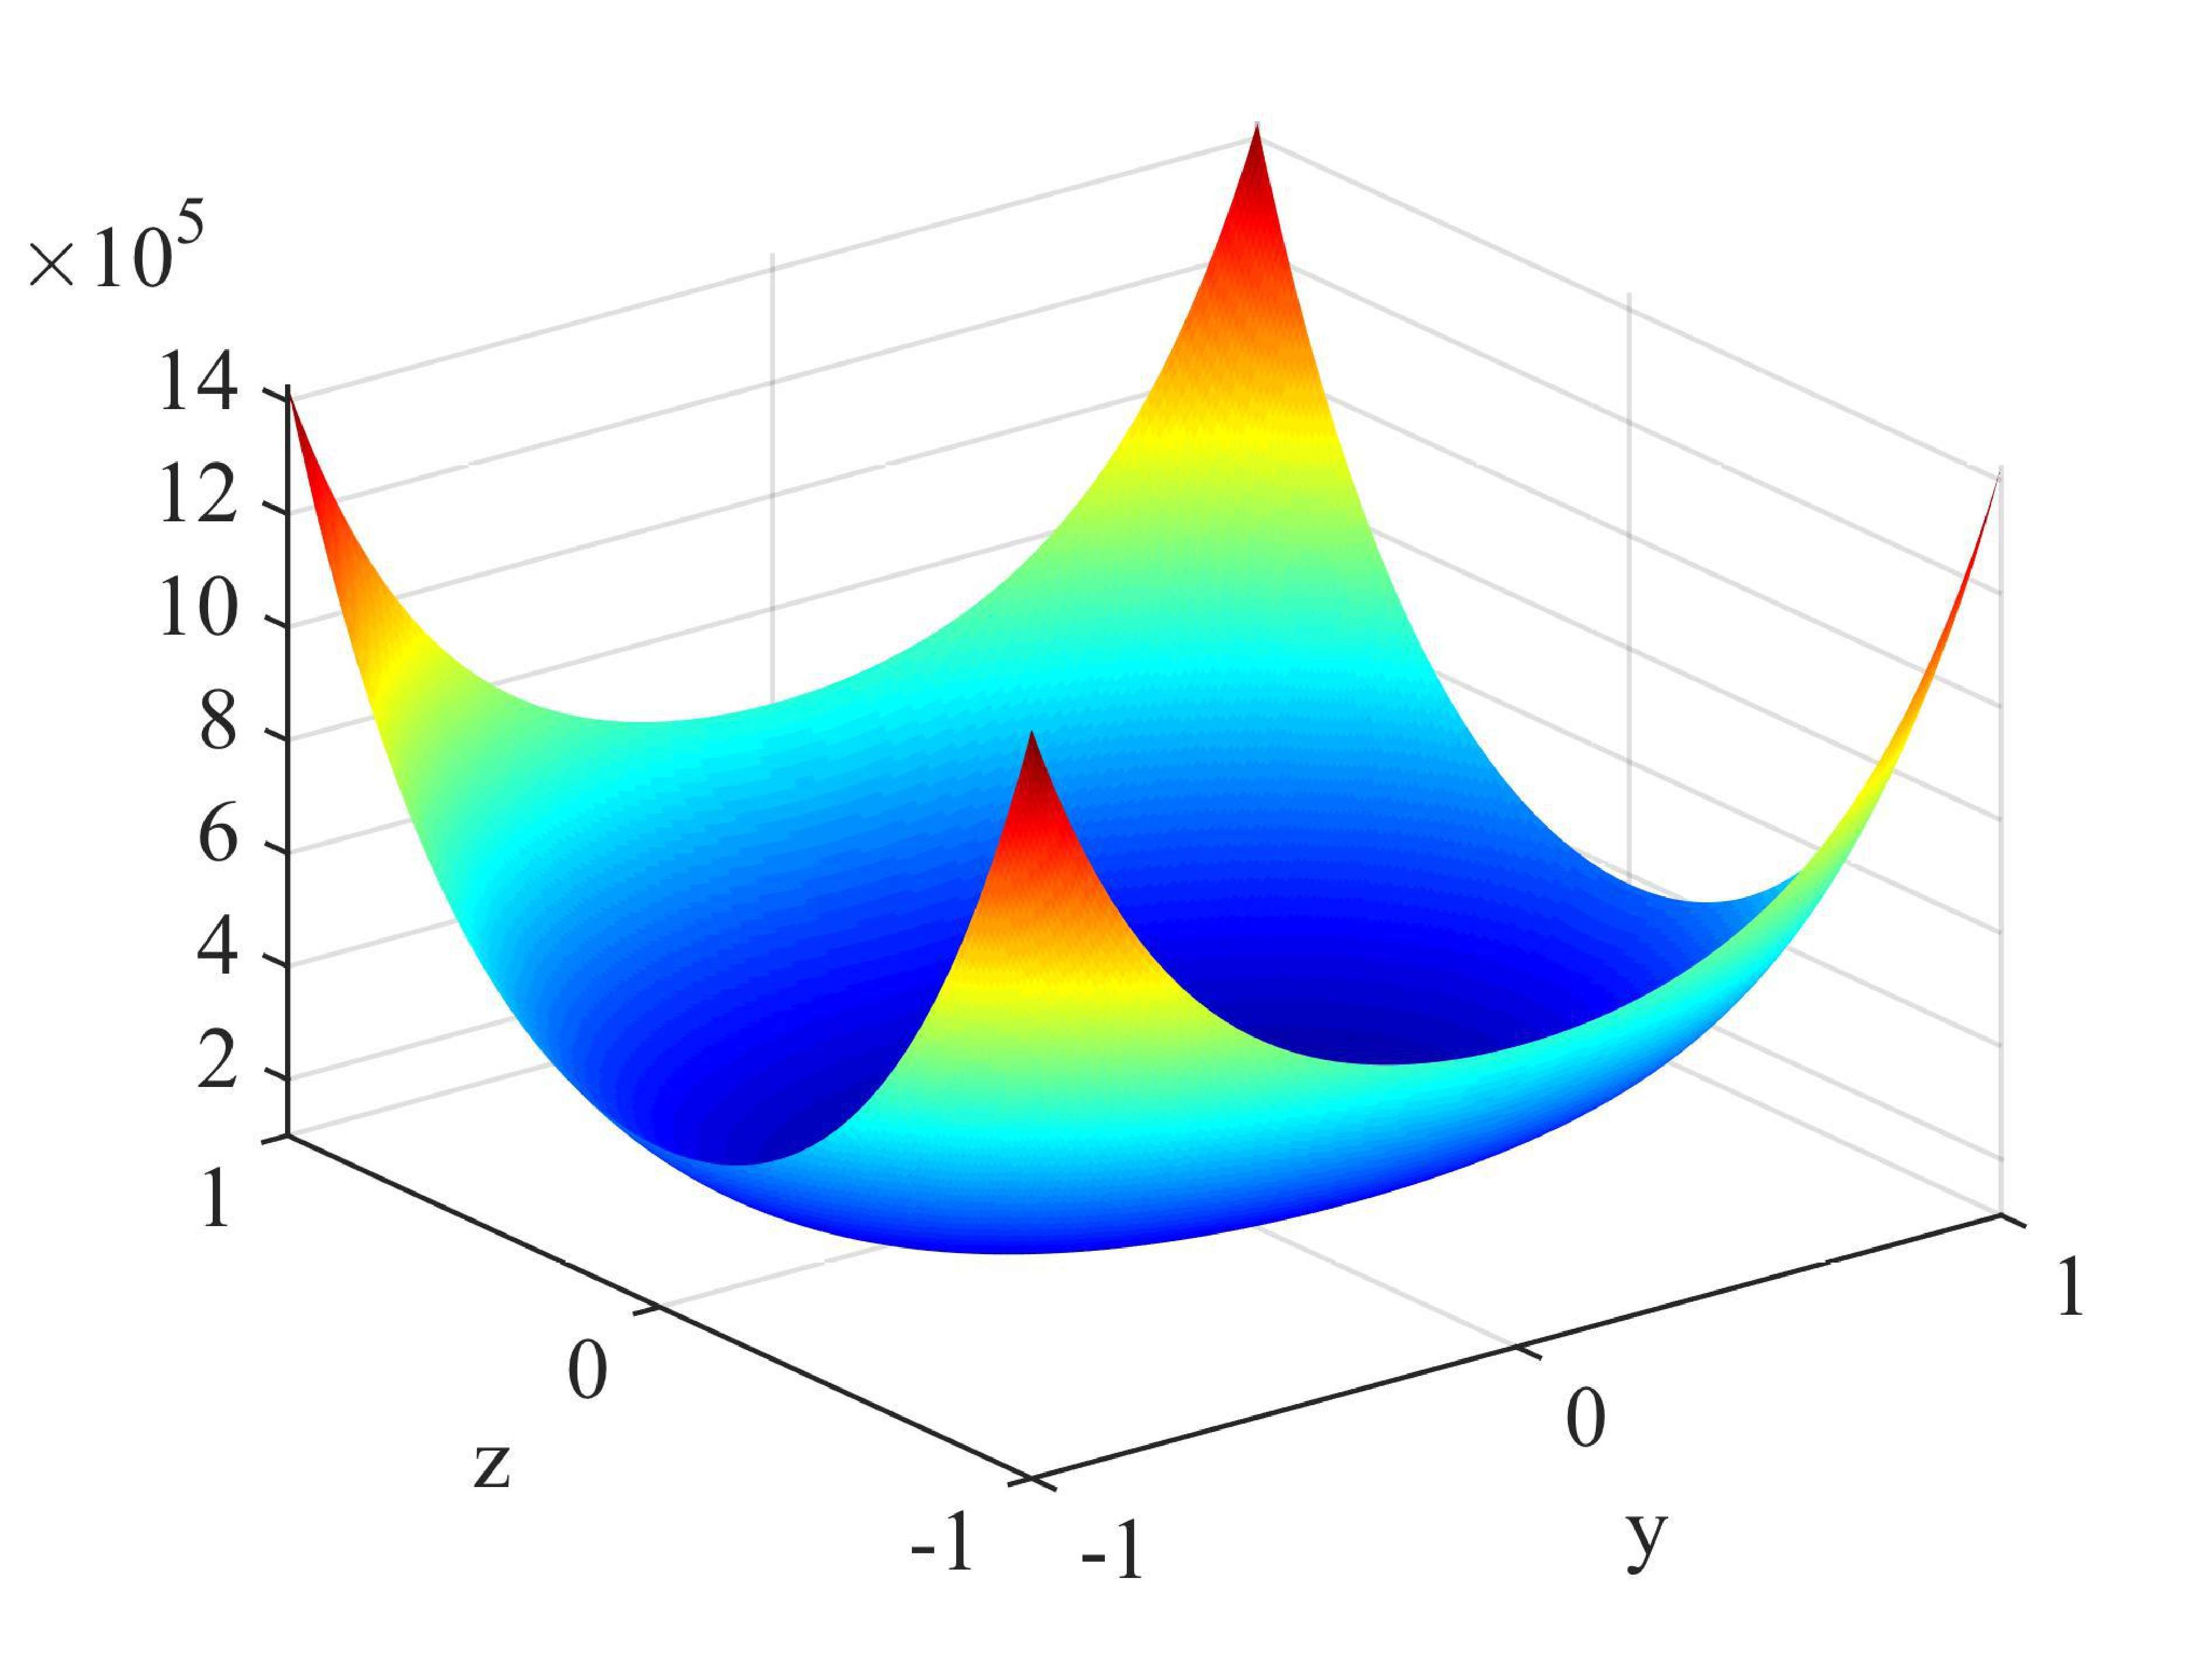
\includegraphics[width=0.45\textwidth]
   {figs/aniso_uniaxial_cartesian_detA_F1p1583.pdf}
 } \subfigure[$F_{11}=1.1954$ (bifurcation)]{
   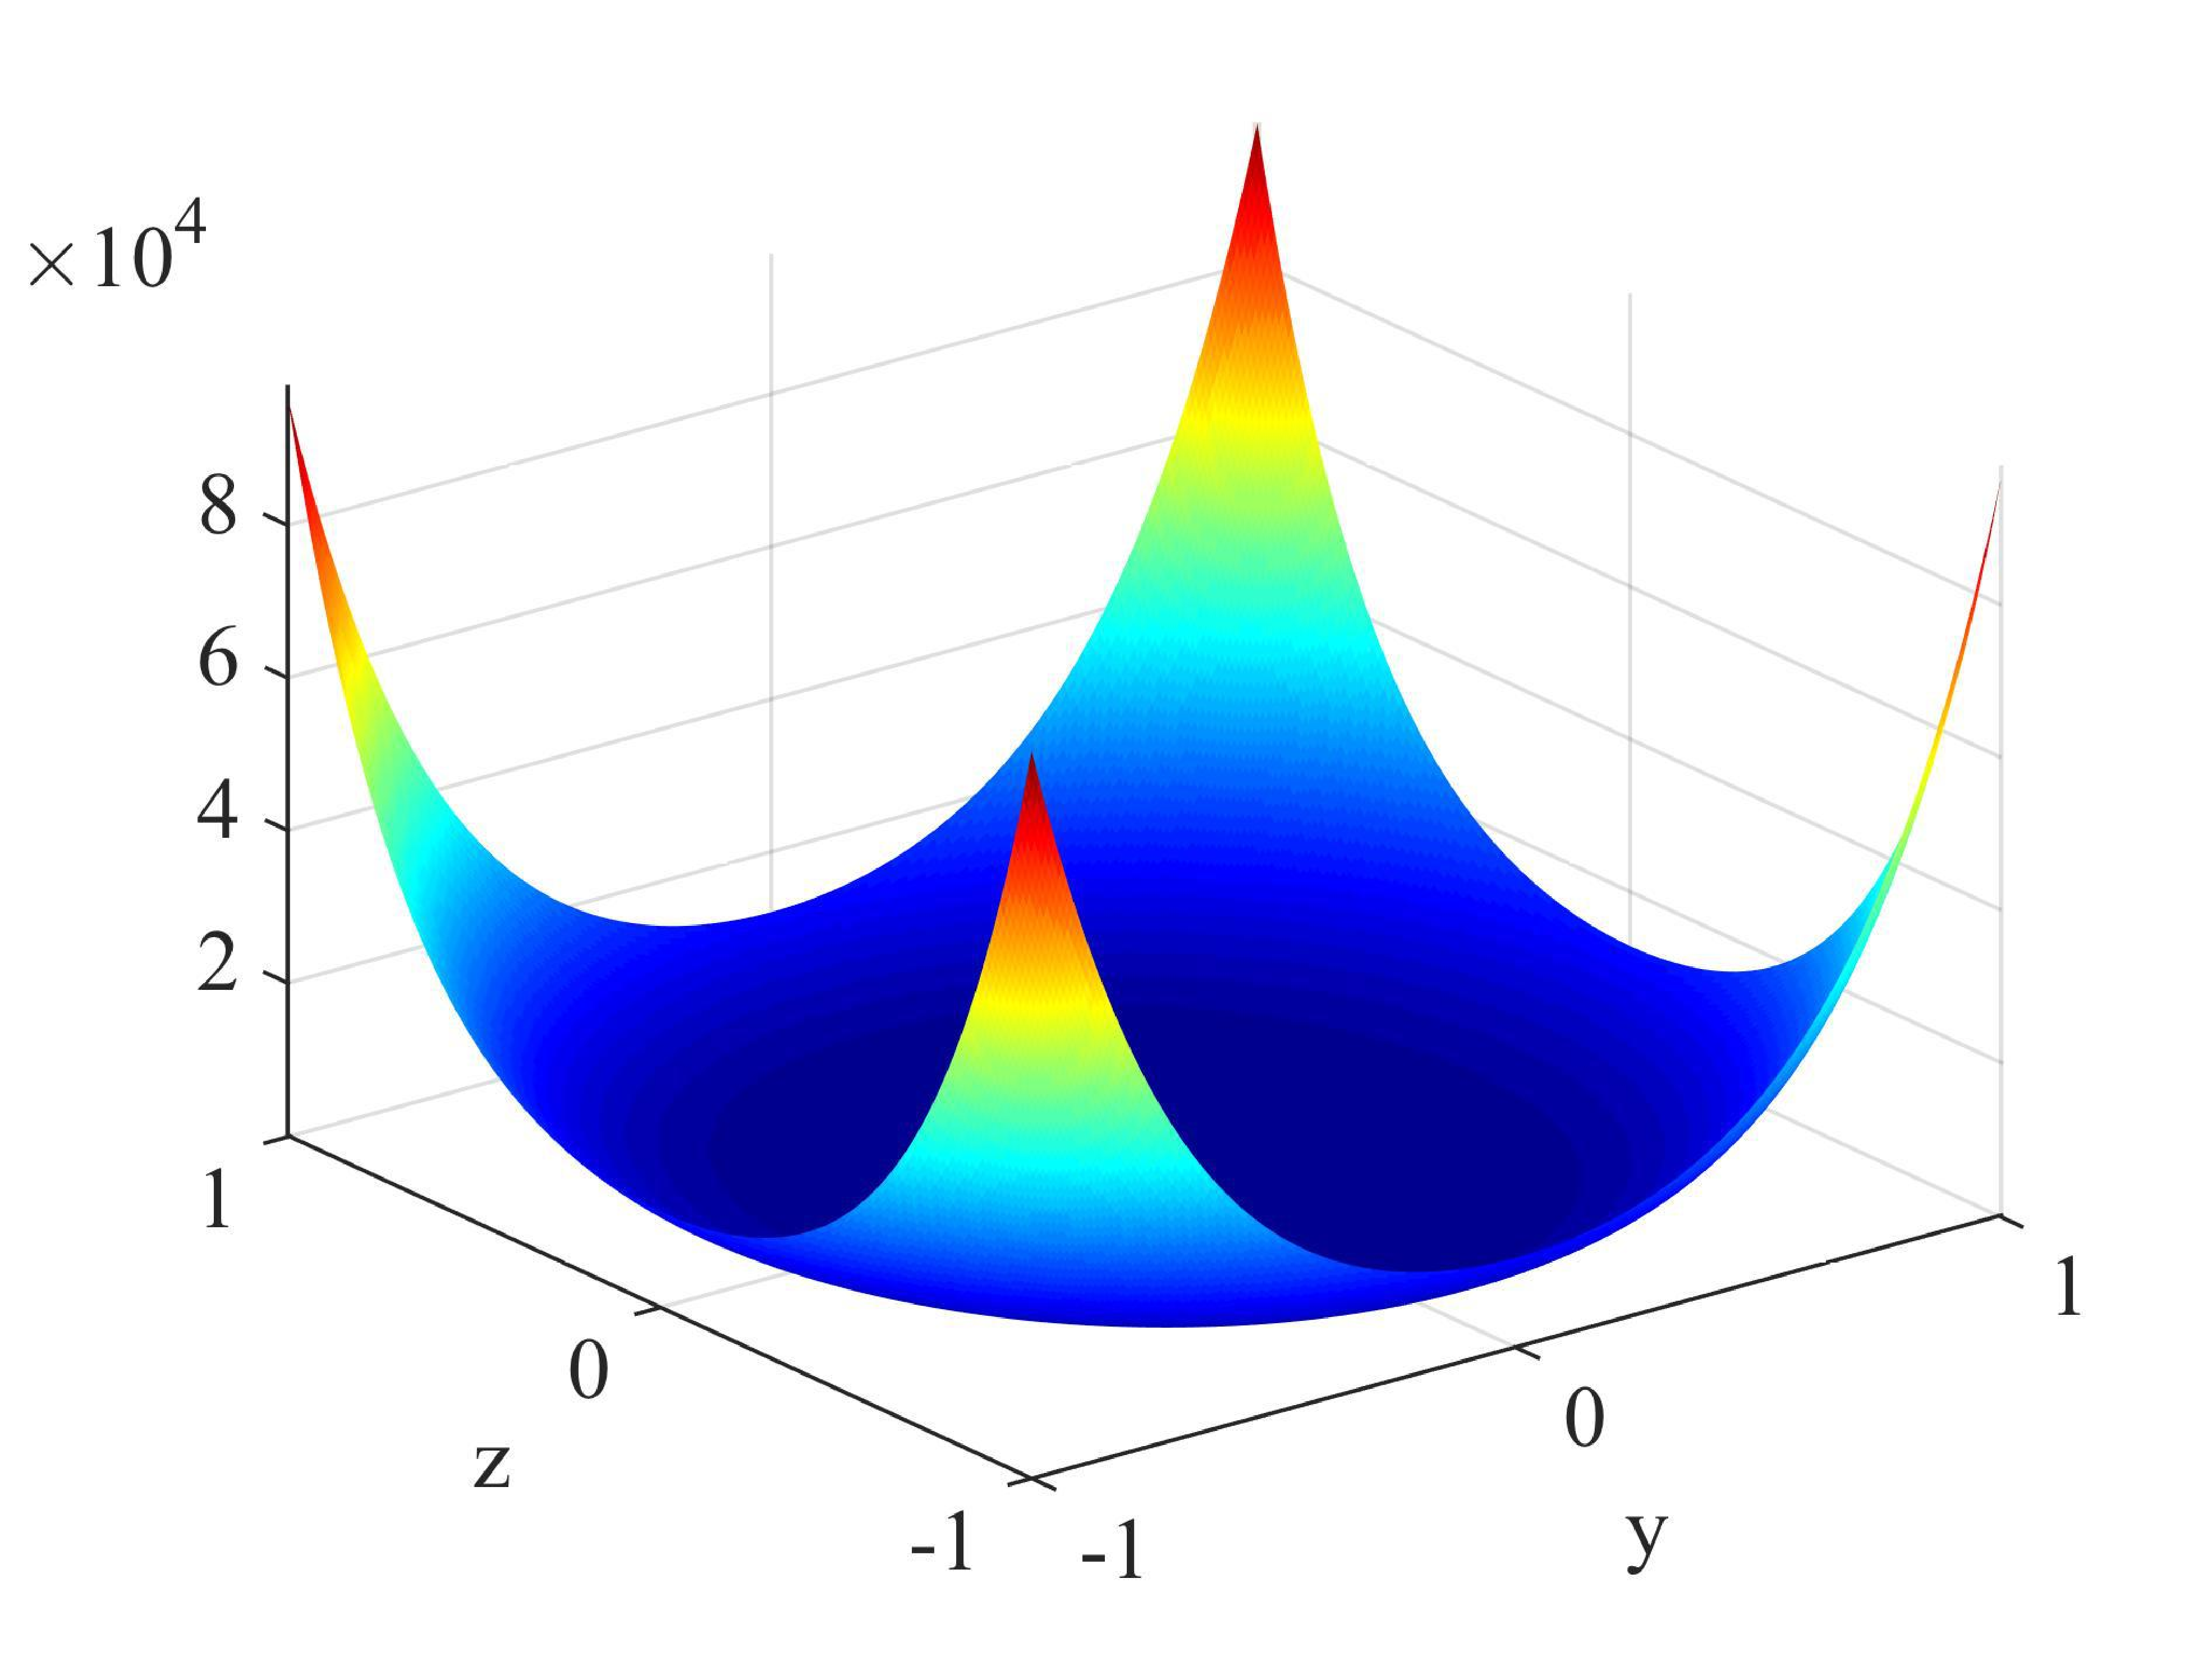
\includegraphics[width=0.45\textwidth]
   {figs/aniso_uniaxial_cartesian_detA_F1p1954.pdf}
 }
   \caption{Cartesian parametrization: landscapes of det$\bA$ 
   for uniaxial tension test on finite deformation anisotropic model at
   different axial stretch levels.}
   \label{fig:aniso_cartesian_detA}
 \end{figure} 

As seen from Figure \ref{fig:aniso_cartesian_detA}, the cartesian 
parametrization again results a simple `bowl-shaped' landscape of det$
\bA$ consistently throughout the loading process, which is in contrast 
to the complex landscapes using alternative parametrizations in 
Figures \ref{fig:aniso_spherical_detA},
\ref{fig:aniso_stereographic_detA} and \ref{fig:aniso_tangent_detA}. 

Similar as in the case of the small deformation model example in 
Section \ref{subsec:isotropic}, the gradient-based optimization 
technique using Newton's iterative solve is more likely to achieve 
convergence, even the initial sweep is performed over a relatively 
coarse grid. The cartesian parametrization is `optimal' in term of trade-off between computational efficiency and robustness. 

In a non-linear large scale finite element simulation, this optimal 
trade-off between computational efficiency and robustness becomes 
critical. The cartesian parametrization could provide a valuable tool 
in material bifurcation analysis. 

\section{Concluding remarks on material point simulations}
Summarizing results from numerical bifurcation analyses on all three
material models, it is found that:

1. The spherical parametrization is the most efficient in terms of
computational cost given the same initial sampling interval, provided
that the initial sampling is fine enough and the initial guess is a
good approximate to the global minimum;

2. The cube parametrization is the most robust one, for all the
material models and sampling intervals, cube parametrization is able
to converge and detect bifurcation; it requires very few initial
sampling points, which could make up for the computational cost;

3. The Lagrange parametrization has similar computational cost as cube
parametrization, but far less robust.

4. The stereographic and exponential parametrization are the least
robust parametrizations, i.e., they are more likely to have
convergence issues, which is expected given the complicated shape of
the minimization function $\det\bA$.

\bibliographystyle{plainnat}
\bibliography{acpami}

\end{document}
